\documentclass[10pt,final]{report}

\usepackage{framed,fancybox}
\usepackage{multicol,verbatim}
\usepackage[pdftex,colorlinks]{hyperref}
\hypersetup{%
colorlinks=true,
linkcolor=black,
urlcolor=cyan
}%
\usepackage{epsfig,enumerate,amsmath,amsfonts,latexsym,graphics,graphicx,theorem,graphics}
\usepackage{fancyhdr,subfigure}
\usepackage{makeidx,amssymb,myfloat,longtable}
\usepackage[dcu]{harvard}
\usepackage[caption2]{ccaption}
\usepackage[bf]{caption2}
\usepackage{palatino}
\newcommand{\hs}[1]{\hspace*{ #1 mm}}
\renewcommand{\bibname}{References}
\renewcommand{\theequation}{\mbox{\thechapter--\arabic{equation}}}
\newtheorem{thm}{Theorem}
\newtheorem{Thmproof}{Proof of Theorem}
\newcommand{\gpops}{$\mathcal{GPOPS}$~}

\newfixedcaption{\examplecaption}{figure}

\theorembodyfont{\upshape}
%\addtolength{\headwidth}{\marginparsep}
%\addtolength{\headwidth}{\marginparwidth}
%\addtolength{\headwidth}{-0.35in}
%\addtolength{\headwidth}{-2.07in}

% \pagestyle{fancyplain}
% \renewcommand{\chaptermark}[1]%
%                  {\markboth{#1}{#1}}
% \renewcommand{\sectionmark}[1]%
%                  {\markright{\thesection\ #1}}
% \lhead[\fancyplain{}{\footnotesize\scshape\thepage}]%
%       {\fancyplain{}{\footnotesize\scshape\rightmark}}
% \rhead[\fancyplain{}{\footnotesize\scshape\leftmark}]%
%       {\fancyplain{}{\footnotesize\scshape\thepage}}
% \cfoot{}

\pagestyle{fancy}
\usepackage{calc}
% \fancyheadoffset[LE,RO]{\marginparsep+\marginparwidth}
\renewcommand{\chaptermark}[1]{\markboth{Chapter \thechapter{.}\: #1}{}}
\renewcommand{\sectionmark}[1]{\markright{\thesection\ #1}}
\fancyhf{}
\fancyhead[LE,RO]{\small\bfseries\thepage}
\fancyhead[LO]{\small\bfseries\rightmark}
\fancyhead[RE]{\small\bfseries\leftmark}
\fancypagestyle{plain}{%
\fancyhead{} % get rid of headers
\renewcommand{\headrulewidth}{0pt} % and the line
}

% \pagestyle{fancy}
% \fancyhead{}
% \fancyfoot{}
% \fancyhead[LO]{\footnotesize\bfseries\MakeUppercase\rightmark}
% \fancyhead[RO,LE]{\footnotesize\bfseries\thepage}
% \fancyhead[RE]{\footnotesize\bfseries\MakeUppercase\leftmark}

\title{{\bf User's Manual for \gpops Version 2.3:} \vspace{12pt}\\
  {\bf A MATLAB$^{\textregistered}$ Software for Solving Multiple-Phase Optimal Control Problems Using the Gauss Pseudospectral Method}}
\author{Anil V.~Rao \\ {\em University of Florida} \\ Gainesville, FL 32607 \\ \\ David Benson \\ {\em The Charles Stark Draper Laboratory, Inc.} \\
  Cambridge, MA 02139 \\ \\ Christopher L.~Darby \\ Camila Francolin \\ Michael Patterson \\ Ilyssa Sanders \\ {\em University of Florida} \\ Gainesville, FL 32607 \\ \\ Geoffrey T.~Huntington \\ {\em Blue Origin, LLC} \\ Seattle, WA \\ \\ 
\vspace{24pt} \\ August 2009}
\date{}

\oddsidemargin=0in
\evensidemargin=0in
\topmargin=1in
\hoffset=0in
\voffset=-1.5in
\textheight=9in
\textwidth=6.5in

\headwidth=\textwidth
\renewcommand{\headrulewidth}{0.25pt}
\raggedbottom

\renewcommand*\captionlabeldelim{\hspace{12pt}}
\newfloat{pfigure}{thp}{lop}[chapter]
\floatname{pfigure}{Figure P\hspace{-2pt}}

\newcounter{example}[chapter]
\newcounter{question}[chapter]
\theoremheaderfont{\bfseries\large\vspace{12pt}}
\theorempreskipamount=1pt
% \theorempostskipamount=0pt
{\theoremstyle{break}\theorembodyfont{\upshape}\newtheorem{example}{Example}[chapter]}
{\theoremstyle{break}\theorembodyfont{\upshape}\newtheorem{solution}{Solution to Example}[chapter]}
% {\theoremstyle{break}\theorembodyfont{\upshape}\newtheorem{question}{Question}[chapter]}
% {\theoremstyle{margin}\theorembodyfont{\upshape}\newtheorem{question}{}[chapter]}
{\theoremstyle{plain}\theoremheaderfont{\normalsize\bfseries}\theorembodyfont{\upshape}\newtheorem{question}{\hspace{-0.25em}}[chapter]}

\newcommand{\examplenumber}{\thechapter--\theexample}
\renewcommand{\theexample}{\thechapter--\arabic{example}}
\renewcommand{\thesolution}{\thechapter--\arabic{solution}}
\renewcommand{\thequestion}{\thechapter--\arabic{question}}
%\newcommand\example{\noindent\vspace{12pt}\stepcounter{example}\bfseries Example \examplenumber\vspace{12pt}\normalfont}
%\newcommand\exchapter{\@startsection{exchapter}{3}{\z@}%
%                                     {-3.25ex\@plus -1ex \@minus -.2ex}%
%                                     {1.5ex \@plus .2ex}%
%                                     {\normalfont\normalsize\bfseries}}
%\newcommand{\example}{\stepcounter{example}\vspace{12pt}\noindent
%  \bfseries Example \theexample \vspace{12pt}\normalfont}
%\newcommand{\solution}{\noindent {\bfseries\large Solution:}}
\newcommand{\ecaption}[1]{\addcontentsline{loe}{example}{\protect\numberline{\theexample}#1}}

% \renewcommand{\theequation}{\thechapter-\arabic{equation}}

\usepackage{color}

\definecolor{shadecolor}{gray}{0.97}
\FrameRule=0.75pt
\FrameSep=5pt
\setlength{\fboxrule}{\FrameRule}
\setlength{\fboxsep}{\FrameSep}

\newenvironment{ovalframe}{%
  \cornersize*{20pt}%
  \setlength{\fboxsep}{6pt}%
  \def\FrameCommand{\ovalbox}%
  \MakeFramed{\advance\hsize-\width \FrameRestore}}%
{\endMakeFramed}

\newenvironment{shadedframe}{%
  \def\FrameCommand{\fcolorbox{black}{shadecolor}}%
%  \MakeFramed {\addtolength{\hsize}{-\width}\FrameRestore}}
  \MakeFramed {\FrameRestore}}
{\endMakeFramed}

\newcommand{\bfblue}[1]{\textcolor{blue}{\bf #1}}
\newcommand{\slred}[1]{\textcolor{red}{\sl #1}}

\makeindex

\begin{document}

\setcounter{tocdepth}{1}
\citationstyle{dcu}

\newcommand{\mygreekbold}{\boldsymbol}
\newcommand{\mybold}{\mathbf}
%\newcommand{\mybold}{\boldsymbol}
% \newcommand{\mybold}{\textbf}
\newcommand{\Ex}{\textbf{E}_x}
\newcommand{\Ey}{\textbf{E}_y}
\newcommand{\Ez}{\textbf{E}_z}
\newcommand{\eQ}{\textbf{e}_Q}
\newcommand{\ex}{\textbf{e}_x}
\newcommand{\ey}{\textbf{e}_y}
\newcommand{\ez}{\textbf{e}_z}
\newcommand{\exprime}{\textbf{e}_x^{\prime}}
\newcommand{\eyprime}{\textbf{e}_y^{\prime}}
\newcommand{\ezprime}{\textbf{e}_z^{\prime}}
\newcommand{\exdprime}{\textbf{e}_x^{\prime\prime}}
\newcommand{\eydprime}{\textbf{e}_y^{\prime\prime}}
\newcommand{\ezdprime}{\textbf{e}_z^{\prime\prime}}
\newcommand{\pone}{\textbf{p}_1}
\newcommand{\ptwo}{\textbf{p}_2}
\newcommand{\pthree}{\textbf{p}_3}
\newcommand{\qone}{\textbf{q}_1}
\newcommand{\qtwo}{\textbf{q}_2}
\newcommand{\qthree}{\textbf{q}_3}
\newcommand{\eone}{\textbf{e}_1}
\newcommand{\etwo}{\textbf{e}_2}
\newcommand{\ethree}{\textbf{e}_3}
\newcommand{\eoneprime}{\eone^{\prime}}
\newcommand{\etwoprime}{\etwo^{\prime}}
\newcommand{\ethreeprime}{\ethree^{\prime}}
\newcommand{\eonedprime}{\eone^{\prime\prime}}
\newcommand{\etwodprime}{\etwo^{\prime\prime}}
\newcommand{\ethreedprime}{\ethree^{\prime\prime}}
\newcommand{\uone}{\textbf{u}_1}
\newcommand{\utwo}{\textbf{u}_2}
\newcommand{\uthree}{\textbf{u}_3}
\newcommand{\Eone}{\textbf{E}_1}
\newcommand{\Etwo}{\textbf{E}_2}
\newcommand{\Ethree}{\textbf{E}_3}
\newcommand{\ux}{\textbf{u}_x}
\newcommand{\uy}{\textbf{u}_y}
\newcommand{\ur}{\textbf{u}_r}
\newcommand{\uth}{\textbf{u}_{\theta}}
\newcommand{\uz}{\textbf{u}_z}
\newcommand{\bfet}{\textbf{e}_t}
\newcommand{\bfeb}{\textbf{e}_b}
\newcommand{\bfen}{\textbf{e}_n}
\newcommand{\dbfet}{\dot{\textbf{e}}_t}
\newcommand{\dfeb}{\dot{\textbf{e}}_b}
\newcommand{\dbfen}{\dot{\textbf{e}}_n}
\newcommand{\eteneb}{\left\{\bfet,\bfen,\bfeb \right\}}
\newcommand{\er}{\textbf{e}_r}
\renewcommand{\eth}{\textbf{e}_{\theta}}
\newcommand{\ephi}{\textbf{e}_{\phi}}
\newcommand{\dg}{\dot{g}}
\newcommand{\dq}{\dot{q}}
\newcommand{\ds}{\dot{s}}
\newcommand{\dx}{\dot{x}}
\newcommand{\dy}{\dot{y}}
\newcommand{\dz}{\dot{z}}
\newcommand{\dbfx}{\dot{\mybold{x}}}
\newcommand{\dbfX}{\dot{\mybold{X}}}
\newcommand{\dbfY}{\dot{\mybold{Y}}}
\newcommand{\dex}{\dot{\textbf{e}}_x}
\newcommand{\dey}{\dot{\textbf{e}}_y}
\newcommand{\dez}{\dot{\textbf{e}}_z}
\newcommand{\deone}{\dot{\textbf{e}}_1}
\newcommand{\detwo}{\dot{\textbf{e}}_2}
\newcommand{\dethree}{\dot{\textbf{e}}_3}
\newcommand{\der}{\dot{\textbf{e}}_r}
\newcommand{\deth}{\dot{\textbf{e}}_{\theta}}
\newcommand{\dEz}{\dot{\textbf{E}}_{z}}
\newcommand{\ddg}{\ddot{g}}
\newcommand{\ddq}{\ddot{q}}
\newcommand{\dr}{\dot{r}}
\newcommand{\dss}{\ddot{s}}
\newcommand{\ddx}{\ddot{x}}
\newcommand{\ddy}{\ddot{y}}
\newcommand{\ddz}{\ddot{z}}
\newcommand{\ddr}{\ddot{r}}
\newcommand{\ddth}{\ddot{\theta}}
\newcommand{\ddbfX}{\ddot{\mybold{X}}}
\newcommand{\ddbfY}{\ddot{\mybold{Y}}}
\newcommand{\Aprime}{A^{\prime}}
\newcommand{\aprime}{a^{\prime}}
\newcommand{\bfb}{\mybold{b}}
\newcommand{\bfbprime}{\mybold{b}^{\prime}}
\newcommand{\bprime}{b^{\prime}}
\newcommand{\bfe}{\textbf{e}}
\newcommand{\bfeprime}{\textbf{e}^{\prime}}
\newcommand{\bfE}{\textbf{E}}
\newcommand{\bfEprime}{\textbf{E}^{\prime}}
\newcommand{\bfEdprime}{\textbf{E}^{\prime\prime}}
\newcommand{\bff}{\mybold{f}}
\newcommand{\bfi}{\mybold{i}}
\newcommand{\bfrho}{\mygreekbold{\rho}}
\newcommand{\rhoprime}{\rho^{\prime}}
\newcommand{\bfp}{\mybold{p}}
\newcommand{\bfq}{\mybold{q}}
\newcommand{\dbfq}{\dot{\mybold{q}}}
\newcommand{\ddbfq}{\ddot{\mybold{q}}}
\newcommand{\bfpbar}{\bar{\mybold{p}}}
\newcommand{\Cprime}{C^{\prime}}
\newcommand{\Pprime}{P^{\prime}}
\newcommand{\Qprime}{Q^{\prime}}
\newcommand{\bfpprime}{\mybold{p}^{\prime}}
\newcommand{\bfr}{\mybold{r}}
\newcommand{\dbfr}{\dot{\bfr}}
\newcommand{\ddbfr}{\ddot{\bfr}}
\newcommand{\bfrbar}{\bar{\mybold{r}}}
\newcommand{\bfu}{\mybold{u}}
\newcommand{\bfU}{\textbf{U}}
\newcommand{\bfupb}{\textbf{b}}
\newcommand{\bfupe}{\textbf{e}}
\newcommand{\bfupf}{\textbf{f}}
\newcommand{\bfupg}{\textbf{g}}
\newcommand{\bfupk}{\textbf{k}}
\newcommand{\bfupkstar}{\textbf{k}^{\ast}}
\newcommand{\bfupkone}{\textbf{k}_1}
\newcommand{\bfupktwo}{\textbf{k}_2}
\newcommand{\bfupkthree}{\textbf{k}_3}
\newcommand{\bfupkonestar}{\textbf{k}^{\ast}_1}
\newcommand{\bfupktwostar}{\textbf{k}^{\ast}_2}
\newcommand{\bfupkthreestar}{\textbf{k}^{\ast}_3}
\newcommand{\bfupx}{\textbf{x}}
\newcommand{\bfupu}{\textbf{u}}
\newcommand{\bfupw}{\textbf{w}}
\newcommand{\bfv}{\mybold{v}}
\newcommand{\dbfv}{\dot{\bfv}}
\newcommand{\bfw}{\mybold{w}}
\newcommand{\bfvprime}{\mybold{v}^{\prime}}
\newcommand{\bfvbar}{\bar{\mybold{v}}}
\newcommand{\bfvbarprime}{\bar{\mybold{v}}^{\prime}}
\newcommand{\bfvhat}{\hat{\bfv}}
\newcommand{\bfvtilde}{\tilde{\bfv}}
\newcommand{\bfphi}{\mybold{\phi}}
\newcommand{\bfx}{\mybold{x}}
\newcommand{\bfa}{\mybold{a}}
\newcommand{\bfc}{\mybold{c}}
\newcommand{\bfabar}{\bar{\mybold{a}}}
\newcommand{\bfg}{\mybold{g}}
\newcommand{\bfh}{\mybold{h}}
\newcommand{\bbC}{\mathbb{C}}
\newcommand{\bbE}{\mathbb{E}}
\newcommand{\bbI}{\mathbb{I}}
\newcommand{\bbO}{\mathbb{O}}
\newcommand{\bbR}{\mathbb{R}}
\newcommand{\bbS}{\mathbb{S}}
\newcommand{\bbT}{\mathbb{T}}
\newcommand{\bbU}{\mathbb{U}}
\newcommand{\bfX}{\mybold{X}}
\newcommand{\bfY}{\mybold{Y}}
\newcommand{\bfupA}{\textbf{A}}
\newcommand{\bfupB}{\textbf{B}}
\newcommand{\bfupC}{\textbf{C}}
\newcommand{\bfupD}{\textbf{D}}
\newcommand{\bfupE}{\textbf{E}}
\newcommand{\bfupEprime}{\textbf{E}^{\prime}}
\newcommand{\bfupF}{\textbf{F}}
\newcommand{\bfupG}{\textbf{G}}
\newcommand{\bfupI}{\textbf{I}}
\newcommand{\bfupK}{\textbf{K}}
\newcommand{\bfupKstar}{\textbf{K}^{\ast}}
\newcommand{\bfupO}{\textbf{O}}
\newcommand{\bfupP}{\textbf{P}}
\newcommand{\bfupQ}{\textbf{Q}}
\newcommand{\bfupS}{\textbf{S}}
\newcommand{\bfupT}{\textbf{T}}
\newcommand{\bfupU}{\textbf{U}}
\newcommand{\bfupV}{\textbf{V}}
\newcommand{\bfupW}{\textbf{W}}
\newcommand{\bfupZ}{\textbf{Z}}
\newcommand{\bfupone}{\textbf{1}}
\newcommand{\bfA}{\mybold{A}}
\newcommand{\bfB}{\mybold{B}}
\newcommand{\bfC}{\mybold{C}}
\newcommand{\bfD}{\mybold{D}}
\newcommand{\bfChat}{\hat{\mybold{C}}}
\newcommand{\bfF}{\mybold{F}}
\newcommand{\bfG}{\mybold{G}}
\newcommand{\bfGdot}{\dot{\mybold{G}}}
\newcommand{\bfGprime}{\mybold{G}^{\prime}}
\newcommand{\bfGbar}{\bar{\mybold{G}}}
\newcommand{\bfGtilde}{\tilde{\mybold{G}}}
\newcommand{\bfFhat}{\hat{\mybold{F}}}
\newcommand{\bfH}{\mybold{H}}
\newcommand{\bfHbar}{\bar{\mybold{H}}}
\newcommand{\bfHprime}{\mybold{H}^{\prime}}
\newcommand{\bfHbarprime}{\bar{\mybold{H}}^{\prime}}
\newcommand{\bfHhat}{\hat{\mybold{H}}}
\newcommand{\bfHbarhat}{\hat{\bar{\mybold{H}}}}
\newcommand{\bfHdot}{\dot{\mybold{H}}}
\newcommand{\bfHbardot}{\dot{\bar{\mybold{H}}}}
\newcommand{\bfI}{\mybold{I}}
\newcommand{\bfK}{\mybold{K}}
\newcommand{\bfLambda}{\boldsymbol{\Lambda}}
\newcommand{\bfGamma}{\boldsymbol{\Gamma}}
\newcommand{\bfM}{\mybold{M}}
\newcommand{\bfMbar}{\bar{\mybold{M}}}
\newcommand{\bfMhat}{\hat{\mybold{M}}}
\newcommand{\bfMbarhat}{\hat{\bar{\mybold{M}}}}
\newcommand{\bfN}{\mybold{N}}
\newcommand{\bfNA}{\mybold{N}_A}
\newcommand{\bfNB}{\mybold{N}_B}
\newcommand{\bfNx}{\mybold{N}_x}
\newcommand{\bfNy}{\mybold{N}_y}
\newcommand{\bfNz}{\mybold{N}_z}
\newcommand{\bfP}{\mybold{P}}
\newcommand{\bfPhat}{\hat{\mybold{P}}}
\newcommand{\bfQ}{\mybold{Q}}
\newcommand{\bfR}{\mybold{R}}
\newcommand{\bfRhat}{\hat{\mybold{R}}}
\newcommand{\bfT}{\mybold{T}}
\newcommand{\bfS}{\mybold{S}}
\newcommand{\bfThat}{\hat{\mybold{T}}}
\newcommand{\bfW}{\mybold{W}}
\newcommand{\bftau}{\mygreekbold{\tau}}
% \newcommand{\bftone}{\mybold{t}_1}
% \newcommand{\bfttwo}{\mybold{t}_2}
\newcommand{\bftone}{\textbf{u}}
\newcommand{\bfttwo}{\textbf{w}}
\newcommand{\bfn}{\textbf{n}}
\newcommand{\dds}[1]{\frac{d{#1}}{ds}}
\newcommand{\ddt}[1]{\frac{d{#1}}{dt}}
\newcommand{\ddtt}[1]{\frac{d^2{#1}}{dt^2}}
\newcommand{\delt}[1]{\frac{\partial{#1}}{\partial t}}
\newcommand{\drdt}{\ddt{\bfr}}
\newcommand{\eonetwothree}{\{\eone,\etwo,\ethree\}}
\newcommand{\Eonetwothree}{\{\Eone,\Etwo,\Ethree\}}
\newcommand{\ponetwothree}{\{\pone,\ptwo,\pthree\}}
\newcommand{\konetwothree}{\{\bfupkone,\bfupktwo,\bfupkthree\}}
\newcommand{\konetwothreestar}{\{\bfupkonestar,\bfupktwostar,\bfupkthreestar\}}
\newcommand{\qonetwothree}{\{\qone,\qtwo,\qthree\}}
\newcommand{\uonetwothree}{\{\uone,\utwo,\uthree\}}
\newcommand{\exyzprime}{\{\exprime,\eyprime,\ezprime\}}
\newcommand{\eonetwothreeprime}{\{\eoneprime,\etwoprime,\ethreeprime\}}
\newcommand{\eonetwothreep}{\{\eone^p,\etwo^p,\ethree^p\}}
\newcommand{\eonetwothreedprime}{\{\eonedprime,\etwodprime,\ethreedprime\}}
\newcommand{\exyz}{\{\ex,\ey,\ez\}}
\newcommand{\Exyz}{\{\ex,\ey,\Ez\}}
\newcommand{\EXYZ}{\{\Ex,\Ey,\Ez\}}
\newcommand{\erthz}{\{\er,\eth,\ez\}}
\newcommand{\Erthz}{\{\er,\eth,\Ez\}}
\newcommand{\erthphi}{\{\er,\eth,\ephi\}}
\newcommand{\erphith}{\{\er,\ephi,\eth\}}
\newcommand{\eQthz}{\{\eQ,\eth,\ez\}}
\newcommand{\etnb}{\{\bfet,\bfen,\bfeb\}}
\newcommand{\ttnn}{\{\bftone,\bfttwo,\bfn\}}
\newcommand{\calph}{\cos\hspace{-0.5pt}\alpha}
\newcommand{\salph}{\sin\hspace{-0.5pt}\alpha}
\newcommand{\talph}{\tan\hspace{-0.5pt}\alpha}
\newcommand{\cbeta}{\cos\hspace{-0.5pt}\beta}
\newcommand{\sbeta}{\sin\hspace{-0.5pt}\beta}
\newcommand{\tbeta}{\tan\hspace{-0.5pt}\beta}
\newcommand{\csqbeta}{\cos^2\hspace{-0.5pt}\beta}
\newcommand{\ssqbeta}{\sin^2\hspace{-0.5pt}\beta}
\newcommand{\cth}{\cos\hspace{-0.5pt}\theta\hspace{1pt}}
\newcommand{\sth}{\sin\hspace{-0.5pt}\theta\hspace{1pt}}
\newcommand{\tth}{\tan\hspace{-0.5pt}\theta\hspace{1pt}}
\newcommand{\secth}{\sec\hspace{-0.5pt}\theta\hspace{1pt}}
\newcommand{\dth}{\dot{\theta}}
\newcommand{\dalpha}{\dot{\alpha}}
\newcommand{\ddalpha}{\ddot{\alpha}}
\newcommand{\uxyz}{\{\ux,\uy,\uz\}}
\newcommand{\ssqth}{\sin^2\hspace{-0.5pt}\theta}
\newcommand{\csqth}{\cos^2\hspace{-0.5pt}\theta}
\newcommand{\secsqth}{\sec^2\hspace{-.51pt}\theta}
\newcommand{\cphi}{\cos\hspace{-0.5pt}\phi}
\newcommand{\sphi}{\sin\hspace{-0.5pt}\phi}
\newcommand{\tphi}{\tan\hspace{-0.5pt}\phi}
\newcommand{\cpsi}{\cos\hspace{-0.5pt}\psi\hspace{1pt}}
\newcommand{\spsi}{\sin\hspace{-0.5pt}\psi\hspace{1pt}}
\newcommand{\dpsi}{\dot{\psi}}
\newcommand{\ddpsi}{\ddot{\psi}}
\newcommand{\dbfbdt}{\frac{d\bfb}{dt}}
\newcommand{\ddbfbdtt}{\frac{d^2\bfb}{dt^2}}
\newcommand{\dbfrdt}{\frac{d\mybold{r}}{dt}}
\newcommand{\ddbfrdtt}{\frac{d^2\mybold{r}}{dt^2}}
\newcommand{\dbfvdt}{\frac{d\mybold{v}}{dt}}
\newcommand{\dphi}{\dot{\phi}}
\newcommand{\ddphi}{\ddot{\phi}}
\newcommand{\ssqphi}{\sin^2\hspace{-0.5pt}\phi}
\newcommand{\csqphi}{\cos^2\hspace{-0.5pt}\phi}
\newcommand{\tsqphi}{\tan^2\hspace{-0.5pt}\phi}
\newcommand{\secphi}{\sec\hspace{-0.5pt}\phi}
\newcommand{\cscphi}{\csc\hspace{-0.5pt}\phi}
\newcommand{\alp}{\mygreekbold{\alpha}}
\newcommand{\bfnu}{\mygreekbold{\nu}}
\newcommand{\bfom}{\mygreekbold{\omega}}
\newcommand{\dbfom}{\dot{\mygreekbold{\omega}}}
\newcommand{\bfomprime}{\mygreekbold{\omega}^{\prime}}
\newcommand{\omprime}{\omega^{\prime}}
\newcommand{\bfOm}{\mygreekbold{\Omega}}
\newcommand{\bfpi}{\mygreekbold{\pi}}
\newcommand{\bfpsi}{\mygreekbold{\psi}}
\newcommand{\omx}{\omega_x}
\newcommand{\omy}{\omega_y}
\newcommand{\omz}{\omega_z}
\newcommand{\omxx}{\omega_{xx}}
\newcommand{\omxy}{\omega_{xy}}
\newcommand{\omxz}{\omega_{xz}}
\newcommand{\omyx}{\omega_{yx}}
\newcommand{\omyy}{\omega_{yy}}
\newcommand{\omyz}{\omega_{yz}}
\newcommand{\omzx}{\omega_{zx}}
\newcommand{\omzy}{\omega_{zy}}
\newcommand{\omzz}{\omega_{zz}}
\newcommand{\omoneone}{\omega_{11}}
\newcommand{\omonetwo}{\omega_{12}}
\newcommand{\omonethree}{\omega_{13}}
\newcommand{\omtwoone}{\omega_{21}}
\newcommand{\omtwotwo}{\omega_{22}}
\newcommand{\omtwothree}{\omega_{23}}
\newcommand{\omthreeone}{\omega_{31}}
\newcommand{\omthreetwo}{\omega_{32}}
\newcommand{\omthreethree}{\omega_{33}}
\newcommand{\omone}{\omega_1}
\newcommand{\omtwo}{\omega_2}
\newcommand{\omthree}{\omega_3}
\newcommand{\lsup}[2]{{\vphantom{#2}}^{#1}{{#2}}}
\newcommand{\lrsup}[3]{{\vphantom{#2}}^{#1}{{#2}}^{#3}}
\newcommand{\lsupddt}[2]{{\vphantom{\frac{d#2}{dt}}}^{#1}{\frac{d#2}{dt}}}
\newcommand{\lsupddtau}[2]{{\vphantom{\frac{d#2}{d\tau}}}^{#1}{\frac{d#2}{d\tau}}}
\newcommand{\lsupdds}[2]{{\vphantom{\frac{d#2}{ds}}}^{#1}{\frac{d#2}{ds}}}
\newcommand{\lrsupddt}[3]{{\vphantom{\frac{d#2}{dt}}}^{#1}{\frac{d#2}{dt}}^{#3}}
\newcommand{\lsupdddtt}[2]{{\vphantom{\frac{d^2#2}{dt^2}}}^{#1}{\frac{d^2#2}{dt^2}}}
\newcommand{\lsupdot}[2]{{\vphantom{\dot{#2}}}^{#1}{\dot{#2}}}
\newcommand{\lsupddot}[2]{{\vphantom{\ddot{#2}}}^{#1}{\ddot{#2}}}
% \newcommand{\dotrel}[1]{\left(\frac{\partial #1}{\partial t}\right)}
% \newcommand{\ddotrel}[1]{\left(\frac{\partial^2{#1}}{\partial t^2}\right)}
\newcommand{\dotrel}[1]{\left(\frac{d #1}{dt}\right)}
\newcommand{\ddotrel}[1]{\left(\frac{d^2{#1}}{dt^2}\right)}
\newcommand{\vdotrel}{\left(\frac{\partial \bfv}{\partial t}\right)}
\newcommand{\rdotcrel}{\left(\frac{\partial \bfr_C}{\partial t}\right)}
\newcommand{\vdotcrel}{\left(\frac{\partial \bfv_C}{\partial t}\right)}
\newcommand{\rdotprel}{\left(\frac{\partial \bfr_P}{\partial t}\right)}
\newcommand{\vdotprel}{\left(\frac{\partial \bfv_P}{\partial t}\right)}
\newcommand{\rhodotrel}{\left(\frac{\partial \bfrho}{\partial t}\right)}
\newcommand{\rhoddotrel}{\left(\frac{\partial^2 \bfrho}{\partial t^2}\right)}
\newcommand{\omdotrel}{\left(\frac{\partial \bfom}{\partial t}\right)}
\newcommand{\omegacrossr}{\mygreekbold{\omega}\times\bfr}
\newcommand{\Omegacrossr}{\mygreekbold{\Omega}\times\bfr}
\newcommand{\omegacrossv}{\mygreekbold{\omega}\times\bfv}
\newcommand{\Omegacrossv}{\mygreekbold{\Omega}\times\bfv}
\newcommand{\bfalpha}{\mygreekbold{\alpha}}
\newcommand{\bfTheta}{\mygreekbold{\Theta}}
\newcommand{\speed}{\|\bfv\|}
\newcommand{\bfzero}{\mybold{0}}
\newcommand{\vhat}{\hat{v}}
\newcommand{\vtilde}{\tilde{v}}
\newcommand{\vprime}{v^{\prime}}
\newcommand{\vbar}{\bar{v}}
\newcommand{\vbarprime}{\bar{v}^{\prime}}
\newcommand{\Chat}{\hat{C}}
\newcommand{\Fhat}{\hat{F}}
\newcommand{\Phat}{\hat{P}}
\newcommand{\Rhat}{\hat{R}}
\newcommand{\That}{\hat{T}}
\newcommand{\dUdr}{\frac{\partial U}{\partial \bfr}}
\newcommand{\mcc}{\mathcal{c}}
\newcommand{\mcg}{\mathcal{g}}
\newcommand{\mcs}{\mathcal{s}}
\newcommand{\mcA}{\mathcal{A}}
\newcommand{\mcB}{\mathcal{B}}
\newcommand{\mcC}{\mathcal{C}}
\newcommand{\mcD}{\mathcal{D}}
\newcommand{\mcE}{\mathcal{E}}
\newcommand{\mcF}{\mathcal{F}}
\newcommand{\mcG}{\mathcal{G}}
\newcommand{\mcK}{\mathcal{K}}
\newcommand{\mcL}{\mathcal{L}}
\newcommand{\mcM}{\mathcal{M}}
\newcommand{\mcN}{\mathcal{N}}
\newcommand{\mcP}{\mathcal{P}}
\newcommand{\mcQ}{\mathcal{Q}}
\newcommand{\mcR}{\mathcal{R}}
\newcommand{\mcT}{\mathcal{T}}
\newcommand{\mcU}{\mathcal{U}}
\newcommand{\mcV}{\mathcal{V}}
\newcommand{\bfmcK}{\mygreekbold{\mathcal{K}}}
\newcommand{\mcS}{\mathcal{S}}
\newcommand{\mcX}{\mathcal{X}}
\newcommand{\mcY}{\mathcal{Y}}
\newcommand{\dmcg}{\dot{\mathcal{g}}}
\newcommand{\ddmcg}{\ddot{\mathcal{g}}}
\newcommand{\dmcs}{\dot{\mathcal{s}}}
\newcommand{\ddmcs}{\ddot{\mathcal{s}}}
\newcommand{\dbfR}{\dot{\bfR}}
\newcommand{\dbfrho}{\dot{\bfrho}}
\newcommand{\ddbfR}{\ddot{\bfR}}
\newcommand{\ddbfrho}{\ddot{\bfrho}}
\newcommand{\eg}{e.g.,~}
\newcommand{\ie}{i.e.,~}
\newcommand{\bbone}{\mathbb{1}}
\newcommand{\pd}[2]{\frac{\partial #1}{\partial #2}}
\newcommand{\pdrf}[3]{\frac{\partial #2}{\hspace{-4pt}\lsup{#1}{\partial #3}}}

\maketitle
\clearpage

\thispagestyle{empty}
\vspace*{6.75in}
\begin{center}
  THIS PAGE IS INTENTIONALLY LEFT BLANK
\end{center}

\chapter*{Acknowledgments}

The software \gpops was developed in response to a demand from
the research and academic community for a customizable implementation
of the Gauss pseudospectral method for solving optimal control
problems.  Indeed, while the authors of \gpops have published
extensively in the open literature on the theory and application of
the Gauss pseudospectral method, no effort has been made to date to
provide source code of actual software that can be utilized and
adapted by a broad community.  The \gpops software is an
attempt to fill that void and enable researchers, educators, and
others involved in solving complex optimal control problems to take
advantage of a code that can be customized to one's particular needs.
The authors of \gpops hope sincerely that the code is useful.

\chapter*{Disclaimer}

This software is provided ``as is'' and free-of-charge.  Neither the
authors nor their employers assume any responsibility for any harm
resulting from the use of this software.  The authors do, however,
hope that users will find this software useful for research and other
purposes.


\chapter*{Preface to The \gpops Software}

It is noted that \gpops has been designed to work with the nonlinear
programming solver SNOPT \cite{Gill1}.  SNOPT can be obtained from one
of the following three sources:  (1) for government, commercial, or
institutional academic use from Stanford Business Software, Inc.; (2)
for individual research use by contacting Professor Philip Gill via
e-mail at pgill@ucsd.edu; (3) For redistribution by contacting the
Office of Technology Licensing at Stanford University. Finally, \gpops
can be adapted to work with other NLP solvers, but these
implementations have not as of yet been developed.

Next, \gpops has the option of using either forward-mode automatic
differentiation or  complex-step differentiation for computing the
objective function gradient and the constraint Jacobian.  Both
complex-step differentiation and forward-mode automatic
differentiation are now {\em built-in options} in \gpops and can be
invoked using the options as specified later in this manual  In
addition, it is noted that earlier versions of \gpops had the ability to
use the following third-party automatic differentiators:
\begin{itemize}
\item Interval Laboratory (INTLAB):  \url{http://www.ti3.tu-harburg.de/rump/intlab/}
\item Matlab Automatic Differentiation (MAD):  \url{http://matlabad.com}
\end{itemize}
INTLAB is developed by Prof.~Siegfried Rump of The University of
Hamburg (Germany) while MAD is a commercial product.

\chapter*{Changes in User Interface from \gpops Versions 1.x}

The user should be aware of the fact that the interface to \gpops has
been revised significantly from \gpops Version 1.x.  In particular,
\gpops 2.x uses a {\em structure-based} interface as opposed to an
interface based on cell arrays.  The new input format has been chosen
because it is more intuitive than the previous input format.  Any
applications that the user has coded using the old input format will
need to be changed to the new format.  These changes should only take
a small effort.

\chapter*{Licensing Agreement}

The software \gpops is distributed under the following license
agreement.  Regardless of how you obtain a copy of \gpops, you must
abide by the following terms:
\verbatiminput{../LICENSE.}

\tableofcontents

\newpage

\chapter{Introduction to Gauss Pseudospectral Optimization Software  (\gpops)}

{\em Gauss Pseudospectral Optimization Software}
(\gpops) is a software program written in MATLAB\footnote{MATLAB is a
  registered trademark of The Mathworks, Inc., One Apple Hill, Natick,
  MA}${}^{\textregistered}$ for solving multiple-phase optimal control
problems of the following form.  Given a set of $P$ phases (where
$p=1,\ldots,P$), minimize the cost functional
\begin{equation}
  J = \sum_{p=1}^{P} J^{(p)} = \sum_{p=1}^{P}
  \left[\Phi^{(p)}(\bfx^{(p)}(t_0),t_0,\bfx^{(p)}(t_f),t_f;\bfq^{(p)})
  + \mcL^{(p)}(\bfx^{(p)}(t),\bfu^{(p)}(t),t;\bfq^{(p)})dt \right]
\end{equation}
subject to the dynamic constraint
\begin{equation}
  \dbfx^{(p)} = \bff^{(p)}(\bfx^{(p)},\bfu^{(p)},t;\bfq^{(p)}), \qquad (p=1,\ldots,P),
\end{equation}
the boundary conditions
\begin{equation}
  \bfphi_{\min} \leq
  \bfphi^{(p)}(\bfx^{(p)}(t_0),t_0^{(p)},\bfx^{(p)}(t_f),t_f^{(p)};\bfq^{(p)})
  \leq \bfphi_{\max}, \qquad (p=1,\ldots,P),
\end{equation}
the inequality path constraints
\begin{equation}
  \bfC^{(p)}(\bfx^{(p)}(t),\bfu^{(p)}(t),t;\bfq^{(p)})\leq  \bfzero, \qquad
  (p=1,\ldots,P),
\end{equation}
and the phase continuity (linkage) constraints
\begin{equation}
  \bfP^{(s)}(\bfx^{(p_l^s)}(t_f),t_f^{(p_l^s)};\bfq^{(p_l^s)},\bfx^{(p_u^s)}(t_0),t_0^{(p_u^s)};\bfq^{(p_u^s)})
  =   \bfzero, \qquad (p_l,p_u\in[1,\ldots,P],s=1,\ldots,L)
\end{equation}
where $\bfx^{(p)}(t)\in\bbR^{n_p}$, $\bfu^{(p)}(t)\in\bbR^{m_p}$,
$\bfq^{(p)}\in\bbR^{q_p}$, and $t\in\bbR$ are, respectively, the state,
control, static parameters, and time in phase $p\in[1,\ldots,P]$, $L$
is the number of phases to be linked,
$p_l^s\in[1,\ldots,P],\;(s=1,\ldots,L)$ are the ``left'' phase numbers,
and $p_u^s\in[1,\ldots,P],\;(s=1,\ldots,L)$ are the ``right'' phase
numbers.

While much of the time a user may want to solve a problem consisting of
multiple phases, it is important to note that the phases
{\em need not be sequential}.  To the contrary, any two phases may be linked
provided that the independent variable does not change direction (\ie the
independent variable moves in the same direction during each phase that is
linked).  A schematic of how phases can potentially be linked is given in
Fig.~\ref{fig: linkages}.
\begin{figure}[h]
  \centering
  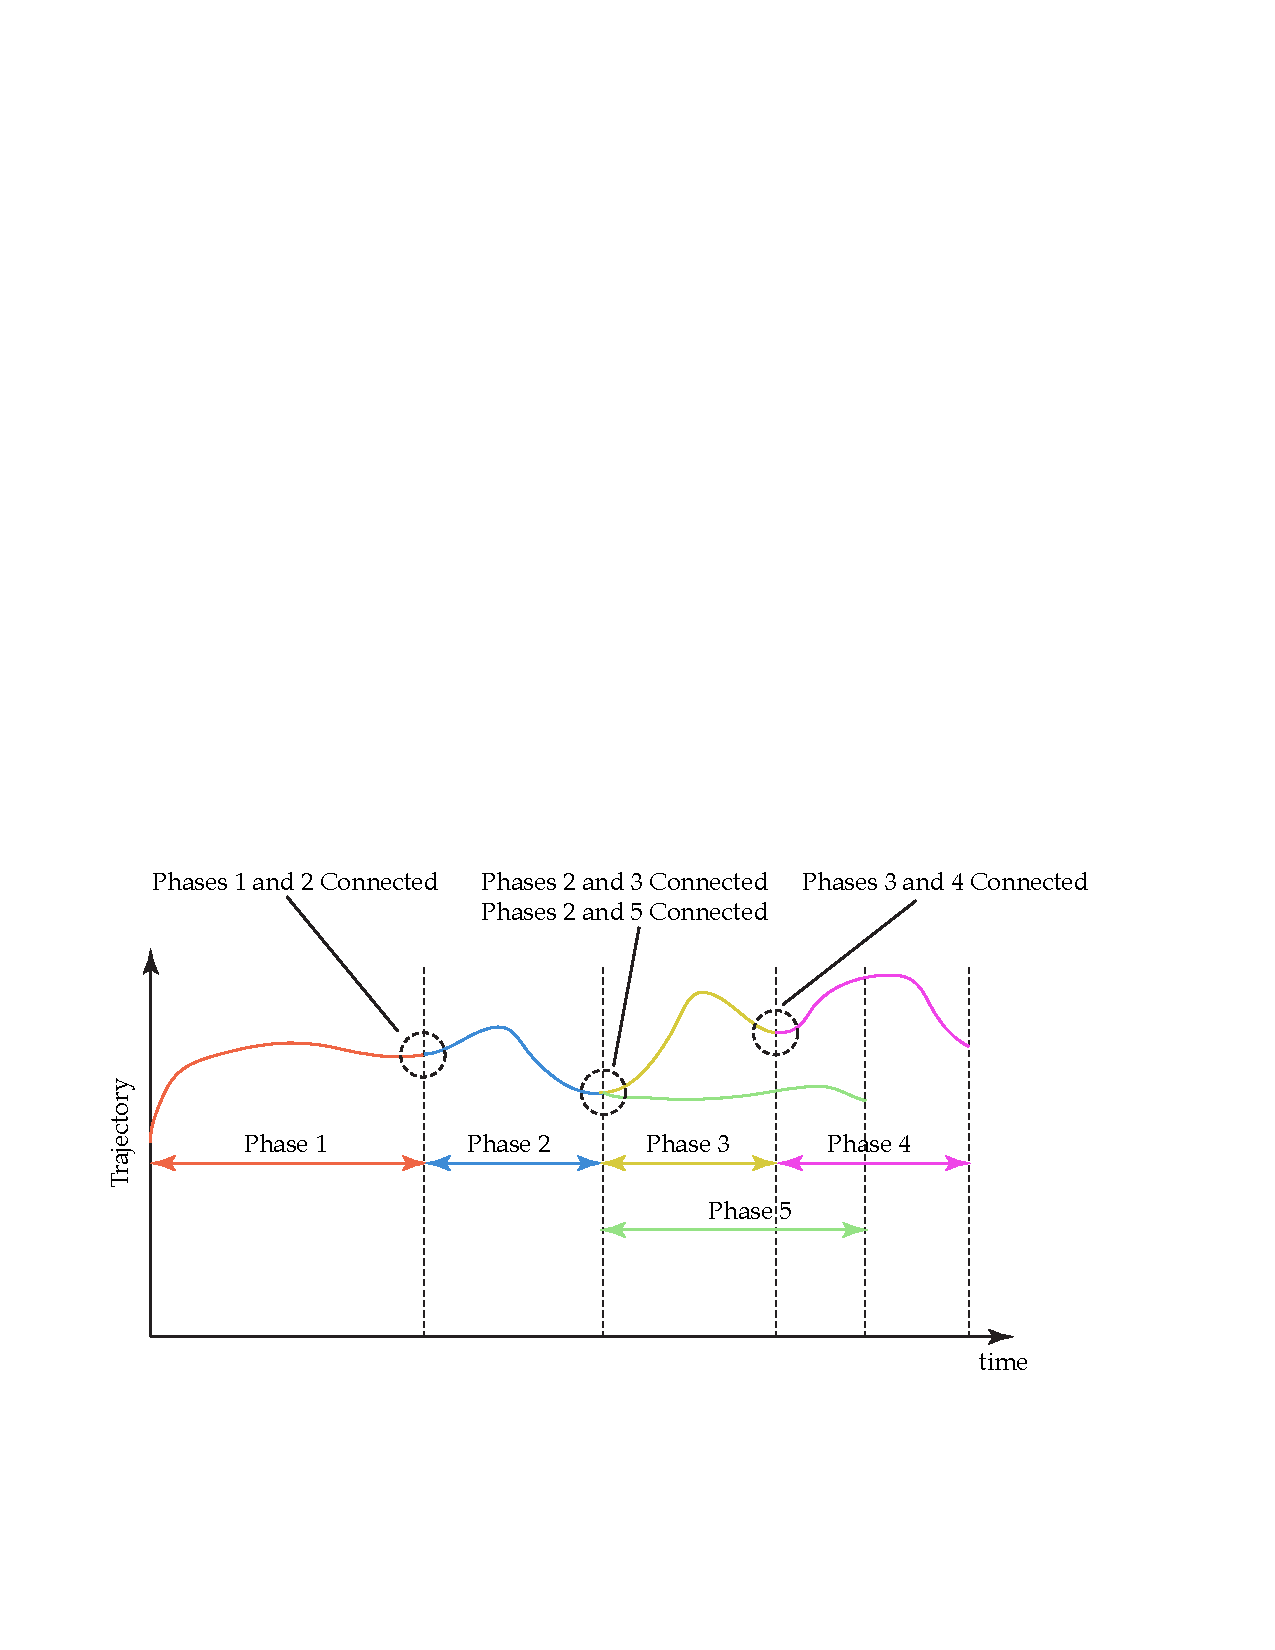
\includegraphics[scale=0.95]{linkages.pdf}
  \caption{Schematic of linkages for multiple-phase optimal control problem.
    The example shown in the picture consists of five phases where the ends of
    phases 1, 2, and 3 are linked to the starts of phases 2, 3, and 4,
    respectively, while the end of phase 3 is linked to the start of phase 5.
    \label{fig: linkages}}
\end{figure}

\section{Gauss Pseudospectral Method Employed by \gpops}

The method employed by \gpops is the {\em Gauss Pseudospectral
Method} (GPM).  The GPM is an orthogonal collocation method where
the collocation points are the {\em Legendre-Gauss} points.  The
theory of the GPM can be found in \cite{Benson1,Benson2,Huntington6} while
applications of the GPM can be found in
\cite{Huntington1,Huntington2,Huntington3,Huntington4}. Strictly
speaking, no knowledge of the GPM is required for using \gpops.
However, for completeness, in this section we describe the
mathematics of the GPM.  It is noted that this section is taken
largely from \citeasnoun{Benson2}.

\subsection{Continuous Bolza Problem \label{Bolza prob}}

Without loss of generality, consider the following optimal control problem.
Determine the state, $\textbf{x}(\tau)\in\mathbb{R}^n$, control,
$\textbf{u}(\tau)\in\mathbb{R}^m$, initial time, $t_0$, and final
time, $t_f$, that minimize the cost functional
\begin{equation}\label{bolza_time_cost}
  J = \Phi(\textbf{x}(-1),t_0,\textbf{x}(1),t_f) + \frac{t_f-t_0}{2}\int_{-1}^{1}
  g(\textbf{x}(\tau),\textbf{u}(\tau),\tau;t_0,t_f) d\tau
\end{equation}
subject to the constraints
\begin{equation}\label{bolza_time_dyn}
  \displaystyle \frac{d \textbf{x}}{d\tau} = \frac{t_f-t_0}{2}
\textbf{f}(\textbf{x}(\tau),\textbf{u}(\tau),\tau;t_0,t_f)
\end{equation}
\begin{equation}\label{bolza_time_bound}
  \boldsymbol{\phi}(\textbf{x}(-1),t_0,\textbf{x}(1),t_f) = \textbf{0}
\end{equation}
\begin{equation}\label{bolza_path}
  \textbf{C}(\textbf{x}(\tau),\textbf{u}(\tau),\tau;t_0,t_f) \leq \textbf{0}
\end{equation}
The optimal control problem of
Eqs.~(\ref{bolza_time_cost})--(\ref{bolza_path}) will be referred to
as the {\em continuous Bolza problem}.  It is noted that the optimal
control problem of Eqs.~(\ref{bolza_time_cost})--(\ref{bolza_path})
can be transformed from the time interval $\tau\in[-1,1]$ to the time
interval $t\in\left[t_0,t_f\right]$ via the affine transformation
\begin{equation}\label{time_map}
  t = \frac{t_f - t_0}{2} \tau + \frac{t_f + t_0}{2}
\end{equation}

\section{Gauss Pseudospectral Discretization of Continuous Bolza Problem
  \label{section: NLP}}

The direct approach to solving the continuous Bolza optimal control
problem of Section \ref{Bolza prob} is to discretize and transcribe
Eqs.~(\ref{bolza_time_cost})--(\ref{bolza_path}) to a nonlinear
programming problem (NLP).  The Gauss pseudospectral method, like
Legendre and Chebyshev methods, is based on approximating the state
and control trajectories using interpolating polynomials.  The state
is approximated using a basis of $N+1$ Lagrange interpolating
polynomials, $L$,
\begin{equation} \label{state approximation gauss}
  \textbf{x}(\tau) \approx \textbf{X}(\tau) = \sum_{i=0}^N
  \textbf{X}(\tau_i) L_i(\tau)
\end{equation}
where $L_i(\tau)\;(i=0,\ldots,N)$ are defined as
\begin{equation}
  L_i(\tau)  = \displaystyle \prod_{j=0,j\neq i}^{N}
  \frac{\tau-\tau_j}{\tau_i-\tau_j}
  \label{lagrange for state}
\end{equation}
Additionally, the control is approximated using a basis of $N$ Lagrange
interpolating polynomials $L_i^*(\tau),\;(i=1,\ldots,N)$ as
\begin{equation} \label{control approximation}
  \textbf{u}(\tau) \approx \textbf{U}(\tau) =
  \sum_{i=1}^N \textbf{U}(\tau_i) L_i^*(\tau)
\end{equation}
where
\begin{equation}\label{lagrange control}
  L_i^*(\tau) = \displaystyle \prod_{j=1,j\neq
  i}^{N}\frac{\tau-\tau_j}{\tau_i-\tau_j}
\end{equation}
It can be seen from Eqs.~(\ref{lagrange
  for state}) and (\ref{lagrange control}) that
$L_i(\tau)\;(i=0,\ldots,N)$ and $L_i^*(\tau)\;(i=1,\ldots,N)$
satisfy the properties
\begin{eqnarray}
  L_i(\tau_j) & = & \left\{\begin{array}{ccc} 1 & , & i=j \\ 0 & , &
      i\neq j \end{array} \right.
  \label{lagrange state property} \\
  L_i^*(\tau_j) & = & \left\{\begin{array}{ccc} 1 & , & i=j \\ 0 & , &
  i\neq j \end{array} \right.
  \label{lagrange costate property}
\end{eqnarray}
Differentiating the expression in Eq.~(\ref{state approximation gauss}), we
obtain
\begin{equation}
  \dot{\textbf{x}}(\tau) \approx \dot{\textbf{X}}(\tau)   =  \sum_{i=0}^N x(\tau_i)
  \dot{L}_i(\tau) \label{derivative state approximation}
\end{equation}
The derivative of each Lagrange polynomial at the LG points can be
represented in a differential approximation matrix,
$D\in\mathbb{R}^{N\times N+1}$.  The elements of the differential
approximation matrix are determined offline as follows:
\begin{equation}
  D_{ki} = \dot L_i(\tau_k) = \sum_{l=0}^N \frac{\displaystyle
    \prod_{j = 0,j \not= i,l}^N (\tau_k - \tau_j)}{\displaystyle
    \prod_{j = 0,j \not= i}^N (\tau_i - \tau_j)}
\end{equation}
where $k = 1,\ldots,N$ and $i = 0,\ldots,N$.  The dynamic constraint
is transcribed into algebraic constraints via the differential
approximation matrix as follows:
\begin{equation}\label{diff_dis_dyn}
    \sum_{i=0}^N D_{ki}
    \textbf{X}_i - \displaystyle\frac{t_f-t_0}{2}
    \textbf{f}(\textbf{X}_k,\textbf{U}_k,\tau_k;t_0,t_f) = \textbf{0} \quad
    (k = 1,\ldots,N)
\end{equation}
where $\textbf{X}_k \equiv \textbf{X}(\tau_k)\in\mathbb{R}^n$ and
$\textbf{U}_k \equiv \textbf{U}(\tau_k)\in\mathbb{R}^m$
$(k=1,\ldots,N$).  Note that the dynamic constraint is collocated
only at the LG points and {\em not} at the boundary
points (this form of collocation differs from other well known
pseudospectral methods such as those found in \cite{Elnagar1} and \cite{Elnagar2}).  Additional
variables in the discretization are defined as follows:
$\textbf{X}_0\equiv\textbf{X}(-1)$, and
$\textbf{X}_f$,  where $\textbf{X}_f$ is
defined in terms of $\textbf{X}_k,\;(k=0,\ldots,N)$ and
$\textbf{U}(\tau_k)\;(k=1,\ldots,N)$ via the Gauss quadrature \cite{Davis1}
\begin{equation} \label{gauss quadrature of xf}
  \textbf{X}_f \equiv \textbf{X}_0 +
  \displaystyle\frac{t_f-t_0}{2}\sum_{k=1}^N w_k
  \textbf{f}(\textbf{X}_k,\textbf{U}_k,\tau_k;t_0,t_f)
\end{equation}
The continuous cost function of Eq.~(\ref{bolza_time_cost}) is
approximated using a Gauss quadrature\cite{Davis1} as
\begin{equation}\label{diff_dis_cost}
    J = \Phi(\textbf{X}_0,t_0,\textbf{X}_f,t_f) + \displaystyle\frac{t_f-t_0}{2}\sum_{k=1}^N w_k g(\textbf{X}_k,\textbf{U}_k,\tau_k;t_0,t_f)
\end{equation}
where $w_k$ are the Gauss weights.  Next, the
boundary constraint of Eq.~(\ref{bolza_time_bound}) is expressed as
\begin{equation}\label{diff_dis_bound}
  \boldsymbol{\phi}(\textbf{X}_0,t_0,\textbf{X}_f,t_f) =
  \textbf{0}
\end{equation}
Furthermore, the path constraint of Eq.~(\ref{bolza_path}) is
evaluated at the LG points as
\begin{equation}\label{diff_dis_path}
  \textbf{C}(\textbf{X}_k,\textbf{U}_k,\tau_k;t_0,t_f) \leq
  \textbf{0} \quad (k = 1,\ldots,N)
\end{equation}
The cost function of Eq.~(\ref{diff_dis_cost}) and the algebraic
constraints of Eqs.~(\ref{diff_dis_dyn}),
(\ref{gauss quadrature of xf}), (\ref{diff_dis_bound}), and
(\ref{diff_dis_path}) define an NLP whose solution is an approximate
solution to the continuous Bolza problem.  Finally, it is noted that the above
discretization can be employed in multiple-phase problems by transcribing the
problem in each phase using the above discretization and connecting the phases
by {\em linkage} constraints (as described above).

\section{KKT Conditions of the NLP\label{KKT Disc Cond}}

The first-order optimality conditions (\ie the Karush-Kuhn-Tucker
(KKT) conditions) of the NLP can be obtained using the augmented cost
function or Lagrangian. The augmented cost function
is formed using the Lagrange multipliers $\boldsymbol{\tilde \Lambda}_k
\in\mathbb{R}^n$, $\boldsymbol{\tilde \mu}_k \in\mathbb{R}^c$, $k =
1,\ldots,N$, $\boldsymbol{\tilde \Lambda_F}\in\mathbb{R}^n$, and
$\boldsymbol{\tilde \nu} \in\mathbb{R}^q$ as
\begin{equation}
  \begin{split}
    J_a & = \Phi(\textbf{X}_0,t_0,\textbf{X}_f,t_f)
    + \displaystyle\frac{t_f-t_0}{2}\sum_{k=1}^N w_k
    g(\textbf{X}_k,\textbf{U}_k,\tau_k;t_0,t_f)
    - \boldsymbol{\tilde \nu}^T
    \boldsymbol{\phi}(\textbf{X}_0,t_0,\textbf{X}_f,t_f) \\
    & -  \displaystyle\sum_{k = 1}^N \boldsymbol{\tilde\mu}_{k}^T
    \textbf{C}(\textbf{X}_k,\textbf{U}_k,\tau_k;t_0,t_f)
    - \displaystyle\sum_{k=1}^N \boldsymbol{\tilde \Lambda}_k^T
    \left(  \sum_{i=0}^N D_{ki}  \textbf{X}_i
      - \displaystyle\frac{t_f-t_0}{2}
    \textbf{f}(\textbf{X}_k,\textbf{U}_k,\tau_k;t_0,t_f) \right) \\
    & - \boldsymbol{\tilde \Lambda_F}^T \left(  \textbf{X}_f -
      \textbf{X}_0 - \displaystyle\frac{t_f-t_0}{2}\sum_{k=1}^N w_k
      \textbf{f}(\textbf{X}_k,\textbf{U}_k,\tau_k;t_0,t_f) \right)
    \end{split}
\end{equation}
The KKT conditions are found by setting equal to zero the derivatives
of the Lagrangian with respect to $\textbf{X}_0$, $\textbf{X}_k$,
$\textbf{X}_f$, $\textbf{U}_k$, $\boldsymbol{\tilde \Lambda}_k$,
$\boldsymbol{\tilde \mu}_k$, $\boldsymbol{\tilde \Lambda_F}$,
$\boldsymbol{\tilde \nu}$, $t_0$, and $t_f$. The solution to the NLP
of Section (\ref{section: NLP}) must satisfy the following KKT conditions:
\begin{eqnarray} \label{kkt 1}
  &  \displaystyle\sum_{i=0}^N
  \textbf{X}_i D_{ki} = \frac{t_f-t_0}{2}
  \textbf{f}_k & \vspace{6pt}\\ \label{kkt 2}
  & \begin{array}{c} \displaystyle\sum_{i=1}^N
    \left(\frac{\boldsymbol{\tilde\Lambda}_i^T}{w_i} +
      \boldsymbol{\tilde \Lambda}^T_F \right)  D^{\dag}_{ki} +
    \boldsymbol{\tilde \Lambda}^T_F  D^{\dag}_{kN+1} = \vspace{6pt}\\
    \label{kkt 3}
    \displaystyle\frac{t_f-t_0}{2} \left(
      -\frac{\partial g_k}{\partial \textbf{X}_k}
      - \left(\frac{\boldsymbol{\tilde\Lambda}_k^T}{w_k} +
        \boldsymbol{\tilde \Lambda}^T_F \right)  \frac{\partial
        \textbf{f}_k}{\partial \textbf{X}_k} +
      \frac{2}{t_f-t_0}\frac{\tilde{\boldsymbol{\mu}}_{k}^T}{w_k}
      \frac{\partial \textbf{C}_{k}}{\partial \textbf{X}_k} \right)
  \end{array} & \vspace{6pt}
\end{eqnarray}
\begin{eqnarray}
  & \textbf{0} = \displaystyle\frac{\partial g_k}{\partial
    \textbf{U}_k} + \left(\frac{\boldsymbol{\tilde\Lambda}_k^T}{w_k} +
    \boldsymbol{\tilde \Lambda}^T_F \right)  \frac{\partial
    \textbf{f}_k}{\partial \textbf{U}_k} -
  \frac{2}{t_f-t_0}\frac{\tilde{\boldsymbol{\mu}}_{k}^T}{w_k}
  \frac{\partial \textbf{C}_{k}}{\partial \textbf{U}_k}  &
    \vspace{6pt}
\end{eqnarray}
\begin{eqnarray}
  \label{kkt 4}
  & \boldsymbol{\phi}(\textbf{X}_0,t_0,\textbf{X}_f,t_f) = \textbf{0}
  & \vspace{6pt}\\
  & \boldsymbol{\tilde \Lambda}_0^T = -\displaystyle\frac{\partial
    \Phi}{\partial \textbf{X}_0} + \boldsymbol{\tilde\nu}^T
  \displaystyle\frac{\partial \boldsymbol{\phi}}{\partial
    \textbf{X}_0} & \vspace{6pt}\\
  \label{kkt 5}
  & \boldsymbol{\tilde \Lambda}_F^T = \displaystyle\frac{\partial
    \Phi}{\partial \textbf{X}_f} - \boldsymbol{\tilde\nu}^T
  \displaystyle\frac{\partial \boldsymbol{\phi}}{\partial
    \textbf{X}_f} &\vspace{6pt}\\
  \label{kkt 6}
  & - \displaystyle\frac{t_f-t_0}{2} \sum_{k = 1}^N w_k
  \frac{\partial \tilde{\cal H}_k}{\partial t_0} + \frac{1}{2}
  \sum_{k=1}^N w_k  \tilde{\cal H}_k
  = \displaystyle\frac{\partial \Phi}{\partial t_0} -
  \boldsymbol{\tilde\nu}^T \frac{\partial
    \boldsymbol{\phi}}{\partial t_0}  &\vspace{6pt}\\
  \label{kkt 7}
  & \displaystyle\frac{t_f-t_0}{2} \sum_{k =
    1}^N w_k  \frac{\partial \tilde{\cal H}_k}{\partial t_f}
  + \frac{1}{2} \sum_{k=1}^N w_k
  \tilde{\cal H}_k = -\displaystyle\frac{\partial \Phi}{\partial
    t_f} + \boldsymbol{\tilde\nu}^T \frac{\partial
    \boldsymbol{\phi}}{\partial
    t_f}  & \vspace{6pt}
\end{eqnarray}
\begin{eqnarray}
  \label{kkt 8}
  &\textbf{C}_k \leq{\bf 0} &\vspace{6pt}\\\label{kkt 9}
  &\tilde\mu_{jk}=0 ,  \; \mbox{when} \quad C_{jk} < 0
  &\vspace{6pt}\\\label{kkt 10}
  &\tilde\mu_{jk}\leq0 , \; \mbox{when} \quad  C_{jk}=0
  &\vspace{6pt}\\\label{kkt 11}
  & \textbf{X}_f = \textbf{X}_0 + \displaystyle\frac{(t_f -
    t_0)}{2} \sum_{k = 1}^N w_k  \textbf{f}_k   &
  \vspace{6pt} \\
  \label{kkt 12}
  & \boldsymbol{\tilde\Lambda}_F = \boldsymbol{\tilde\Lambda}_0 +
  \displaystyle\frac{t_f-t_0}{2} \sum_{k = 1}^N w_k  \left(
    -\frac{\partial g_k}{\partial \textbf{X}_k} -
    \left(\frac{\boldsymbol{\tilde\Lambda}_k^T}{w_k} +
      \boldsymbol{\tilde \Lambda}^T_F \right)  \frac{\partial
      \textbf{f}_k}{\partial \textbf{X}_k} + \frac{2}{t_f-t_0}
    \frac{\tilde{\boldsymbol{\mu}}_k^T}{w_k}
    \frac{\partial \textbf{C}_k}{\partial \textbf{X}_k} \right)
\end{eqnarray}
where the shorthand
notation $g_k \equiv g(\textbf{X}_k,\textbf{U}_k,\tau_k;t_0,t_f)$, $\textbf{f}_k \equiv
\textbf{f}(\textbf{X}_k,\textbf{U}_k,\tau_k;t_0,t_f)$, \\ ${\cal H}_k \equiv {\cal H}(
\textbf{X}_k,\boldsymbol{\Lambda}_k,\boldsymbol{\mu}_k,\textbf{U}_k,\tau_k;t_0,t_f)$,
and $C_{jk} \equiv C_j(\textbf{X}_k,\textbf{U}_k,\tau_k;t_0,t_f)$ is
used. Note that the augmented Hamiltonian, $\tilde {\cal H}_k$, is defined as
\begin{equation}
\tilde {\cal H}_k \equiv g_k +
\left(\displaystyle\frac{\boldsymbol{\tilde\Lambda}_k^T}{w_k} +
\boldsymbol{\tilde \Lambda}^T_F \right)  \textbf{f}_k -
    \frac{2}{t_f-t_0}\frac{\tilde{\boldsymbol{\mu}}_k^T}{w_k}
     \textbf{C}_k
 \end{equation}
and $\boldsymbol{\tilde \Lambda}_0$ is defined as
\begin{equation}\label{KKT_costate_0}
  \boldsymbol{\tilde \Lambda}_0^T \equiv - \displaystyle\frac{\partial
    \Phi}{\partial \textbf{X}_0} + \boldsymbol{\tilde \nu}^T
  \frac{\partial \boldsymbol{\phi}}{\partial \textbf{X}_0}
\end{equation}

\section{First-Order Optimality Conditions of Continuous Bolza Problem
  \label{variational cond}}

The indirect approach to solving the continuous Bolza problem of
Eqs.~(\ref{bolza_time_cost})--(\ref{bolza_path}) in
Section~\ref{Bolza prob} is to apply the calculus of variations and
Pontryagin's Maximum Principle \cite{Pontryagin1} to obtain
first-order necessary conditions for optimality \cite{Kirk1}.   These
variational conditions are typically derived using the augmented
Hamiltonian, ${\cal H}$, defined as
\begin{equation}
{\cal
  H}(\textbf{x},\boldsymbol{\lambda},\boldsymbol{\mu},\textbf{u},\tau;t_0,t_f)
  = g(\textbf{x},\textbf{u},\tau;t_0,t_f) +
  \boldsymbol{\lambda}^T(\tau)\textbf{f}(\textbf{x},\textbf{u},\tau;t_0,t_f)
  - \boldsymbol{\mu}^T(\tau)  \textbf{C}(\textbf{x},\textbf{u},\tau;t_0,t_f)
\end{equation}
where $\boldsymbol{\lambda}(\tau) \in\mathbb{R}^n$ is the costate and
$\boldsymbol{\mu}(\tau) \in\mathbb{R}^c$ is the Lagrange multiplier
associated with the path constraint.  The continuous-time first-order
optimality conditions can be shown to be
\begin{equation}\label{necc_cond}\begin{array}{c}
\displaystyle\frac{d \textbf{x}}{d\tau} =
\displaystyle\frac{t_f-t_0}{2}\textbf{f}(\textbf{x},\textbf{u},\tau;t_0,t_f)
= \frac{t_f-t_0}{2}\displaystyle\frac{\partial {\cal H}}{\partial
  \boldsymbol{\lambda}} \vspace{6pt}\\
\displaystyle\frac{d \boldsymbol{\lambda}}{d\tau} =
\displaystyle\frac{t_f-t_0}{2}\left(-\frac{\partial g}{\partial
    \textbf{x}} - \boldsymbol{\lambda}^T \frac{\partial
    \textbf{f}}{\partial \textbf{x}} + \boldsymbol{\mu}^T
\frac{\partial \textbf{C}}{\partial \textbf{x}}\right) =
-\displaystyle\frac{t_f-t_0}{2} \displaystyle\frac{\partial {\cal
    H}}{\partial \textbf{x}}
\vspace{6pt}\\
\textbf{0} = \displaystyle\frac{\partial g}{\partial \textbf{u}} +
\boldsymbol{\lambda}^T \frac{\partial \textbf{f}}{\partial \textbf{u}}
- \boldsymbol{\mu}^T  \frac{\partial \textbf{C}}{\partial
  \textbf{u}} = \displaystyle\frac{\partial {\cal H}}{\partial
  \textbf{u}} \vspace{6pt}\\
\boldsymbol{\phi}(\textbf{x}(\tau_0),t_0,\textbf{x}(\tau_f),t_f) =
\textbf{0} \vspace{6pt}\\
\boldsymbol{\lambda}(\tau_0) = -\displaystyle\frac{\partial
\Phi}{\partial \textbf{x}(\tau_0)} + \boldsymbol{\nu}^T
\displaystyle\frac{\partial \boldsymbol{\phi}}{\partial
  \textbf{x}(\tau_0)} \;\; , \;\;
\boldsymbol{\lambda}(\tau_f) = \displaystyle\frac{\partial
\Phi}{\partial \textbf{x}(\tau_f)} - \boldsymbol{\nu}^T
\displaystyle\frac{\partial \boldsymbol{\phi}}{\partial
\textbf{x}(\tau_f)} \vspace{6pt}\\
{\cal H}(t_0) = \displaystyle\frac{\partial \Phi}{\partial t_0} -
\boldsymbol{\nu}^T \frac{\partial \boldsymbol{\phi}}{\partial
t_0}  \; \; , \; \;
{\cal H}(t_f) = -\displaystyle\frac{\partial \Phi}{\partial t_f} +
\boldsymbol{\nu}^T \frac{\partial \boldsymbol{\phi}}{\partial
t_f}  \vspace{6pt}\\
 \mu_j(\tau)=0 , \; \mbox{when} \quad
 C_{j}(\textbf{x},\textbf{u},\tau;t_0,t_f)
 < 0 , \quad j = 1,\ldots,c \vspace{6pt}\\
 \mu_j(\tau)\leq0 , \; \mbox{when} \quad
 C_{j}(\textbf{x},\textbf{u},\tau;t_0,t_f)=0 , \quad j = 1,\ldots,c
\end{array}\end{equation}
where $\boldsymbol{\nu} \in\mathbb{R}^q$ is Lagrange multiplier
associated with the boundary condition $\boldsymbol{\phi}$.  It can be
shown that the augmented Hamiltonian at the initial and final times
can be written, respectively, as
\begin{eqnarray}
  {\cal H}(t_0) & =& -\frac{t_f - t_0}{2}\int_{-1}^1 \frac{
    \partial {\cal H}}{\partial t_0}d\tau +
  \frac{1}{2}\int_{-1}^1 {\cal H} d\tau
  \label{initial Hamiltonian} \\
  {\cal H}(t_f) & = &  \frac{t_f - t_0}{2}\int_{-1}^1 \frac{
      \partial {\cal H}}{\partial t_f}d\tau +
    \frac{1}{2}\int_{-1}^1 {\cal H} d\tau
    \label{final Hamiltonian}
\end{eqnarray}

\section{Gauss Pseudospectral Discretized Necessary Conditions\label{Disc Nec Cond}}

In order to discretize the variational conditions of Section
(\ref{variational cond}) using the Gauss pseudospectral
discretization, it is necessary to form an appropriate approximation
for the costate.  In this method, the costate, $\lambda(\tau)$, is
approximated as follows:
\begin{equation}
  \lambda(\tau) \approx \Lambda(\tau) =   \sum_{i=1}^{N+1}
  \lambda(\tau_i) L_i^\dag(\tau)
  \label{costate approximation}
\end{equation}
where $L_i^{\dag}(\tau)\;(i=1,\ldots,N+1)$ are defined as
\begin{equation}
  L_i^{\dag}(\tau) = \displaystyle \prod_{j=1,j\neq i}^{N+1}
  \frac{\tau-\tau_j}{\tau_i-\tau_j}
  \label{lagrange for costate}
\end{equation}
It is emphasized that the costate approximation is {\em different}
from the state approximation.  In particular, the basis of $N+1$
Lagrange interpolating polynomials
$L_i^{\dag}(\tau)\;(i=1,\ldots,N+1)$ includes the costate at the
{\em final} time (as opposed to the initial time which is used in the
state approximation).  This (non-intuitive) costate approximation is
necessary in order to provide a complete mapping between the KKT
conditions and the variational conditions.

Using the costate approximation of Eq.~(\ref{costate approximation}), The
first-order necessary conditions of the continuous Bolza
problem in Eq.~(\ref{necc_cond}) are discretized as follows.  First,
the state and control are approximated using Eqs.~(\ref{state
approximation gauss}) and (\ref{control approximation}),
respectively.  Next, the costate is approximated using the basis of
$N+1$ Lagrange interpolating polynomials as defined in
Eq.~(\ref{costate approximation}).  The continuous-time first-order
optimality conditions of Eq.~(\ref{necc_cond}) are discretized using
the variables $\textbf{X}_0\equiv\textbf{X}(-1)$, $\textbf{X}_k \equiv
\textbf{X}(\tau_k) \in\mathbb{R}^n$, and
$\textbf{X}_f\equiv\textbf{X}(1)$ for the state, $\textbf{U}_k
\equiv \textbf{U}(\tau_k) \in\mathbb{R}^m$ for the control,
$\boldsymbol{\Lambda}_0\equiv\boldsymbol{\Lambda}(-1)$,
$\boldsymbol{\Lambda}_k \equiv
\boldsymbol{\Lambda}(\tau_k)\in\mathbb{R}^n$, and
$\boldsymbol{\Lambda}_f\equiv\boldsymbol{\Lambda}(1)$ for the costate,
and $\boldsymbol{\mu}_k\equiv\boldsymbol{\mu}(\tau_k)
\in\mathbb{R}^c$, for the Lagrange multiplier associated with
the path constraints at the LG points $k = 1,\ldots,N$.  The other
unknown variables in the problem are the initial and final times,
$t_0 \in\mathbb{R}$, $t_f \in \mathbb{R}$, and the Lagrange
multiplier, $\boldsymbol{\nu} \in \mathbb{R}^q$.  The total number of
variables is then given as $(2n+m+c)N+4n+q+2$.  These variables are
used to discretize the continuous necessary conditions of
Eq.~(\ref{necc_cond}) via the Gauss pseudospectral discretization.
Note that the derivative of the state is approximated using Lagrange
polynomials based on $N+1$ points consisting of the $N$ LG points
and the initial time, $\tau_0$, while the derivative of the costate is
approximated using Lagrange polynomials based on $N+1$ points
consisting of the $N$ LG points and the final time, $\tau_f$.  The
resulting algebraic equations that approximate the continuous
necessary conditions at the LG points are given as
\begin{eqnarray} \label{dis_ness_state}
& \displaystyle\sum_{i=0}^N
\textbf{X}_i D_{ki} = \frac{t_f-t_0}{2}  \textbf{f}_k
 & \vspace{6pt}\\  &
\displaystyle\sum_{i=1}^N \boldsymbol{\Lambda}_i D^\dag_{ki} +
\boldsymbol{\Lambda}_f  D^\dag_{kN+1} =
\displaystyle\frac{t_f-t_0}{2} \left(
 -\frac{\partial g_k}{\partial \textbf{X}_k}
- \boldsymbol{\Lambda}^T_k  \frac{\partial
\textbf{f}_k}{\partial \textbf{X}_k} + \boldsymbol{\mu}_k^T
\frac{\partial \textbf{C}_k}{\partial \textbf{X}_k} \right)  & \vspace{6pt}\\
\label{hbvp discrete 2}
& \textbf{0} = \displaystyle\frac{\partial g_k}{\partial \textbf{U}_k}
+ \boldsymbol{\Lambda}^T_k  \frac{\partial
\textbf{f}_k}{\partial \textbf{U}_k} - \boldsymbol{\mu}_k^T
\frac{\partial \textbf{C}_k}{\partial \textbf{U}_k}   & \vspace{6pt}\\
\label{hbvp discrete 3}
& \boldsymbol{\phi}(\textbf{X}_0,t_0,\textbf{X}_f,t_f) = \textbf{0} \\
& \boldsymbol{\Lambda}_0 = -\displaystyle\frac{\partial
\Phi}{\partial \textbf{X}_0} + \boldsymbol{\nu}^T
\displaystyle\frac{\partial \boldsymbol{\phi}}{\partial
  \textbf{X}_0} & \vspace{6pt} \\
\label{hbvp discrete 4}
& \boldsymbol{\Lambda}_f = \displaystyle\frac{\partial
\Phi}{\partial \textbf{X}_f} - \boldsymbol{\nu}^T
\displaystyle\frac{\partial \boldsymbol{\phi}}{\partial
\textbf{X}_f} &\vspace{6pt}\\ \label{initial_H} & -
\displaystyle\frac{t_f-t_0}{2} \sum_{k = 1}^N w_k
\frac{\partial {\cal H}_k}{\partial t_0}  +
\frac{1}{2} \sum_{k=1}^N w_k  {\cal H}_k =
\displaystyle\frac{\partial \Phi}{\partial t_0} -
\boldsymbol{\nu}^T \frac{\partial
\boldsymbol{\phi}}{\partial t_0}  &\vspace{6pt} \\
\label{final_H} & \displaystyle\frac{t_f-t_0}{2} \sum_{k = 1}^N
w_k  \frac{\partial {\cal H}_k}{\partial t_f}  + \frac{1}{2}
\sum_{k=1}^N w_k  {\cal H}_k =
-\displaystyle\frac{\partial \Phi}{\partial t_f} +
\boldsymbol{\nu}^T \frac{\partial \boldsymbol{\phi}}{\partial
t_f}  & \vspace{6pt}\\
& \mu_{jk}=0 ,  \; \mbox{when} \quad C_{jk} < 0  &\vspace{6pt}\\\label{hbvp discrete 6}
& \mu_{jk}\leq0 , \; \mbox{when} \quad  C_{jk}=0  &\label{hbvp discrete 7}
\end{eqnarray}
for $k = 1,\ldots,N$ and $j = 1,\ldots,c$. The final two
equations that are required (in order to link the initial and final
state and costate, respectively) are
\begin{eqnarray}
  & \textbf{X}_f = \textbf{X}_0 + \displaystyle\frac{t_f -
    t_0}{2} \sum_{k = 1}^N w_k  \textbf{f}_k &  \vspace{6pt}
  \label{dis_ness_state_bound} \\
  & \boldsymbol{\Lambda}_f = \boldsymbol{\Lambda}_0 +
  \displaystyle\frac{t_f-t_0}{2} \sum_{k = 1}^N w_k  \left(
    -\frac{\partial g_k}{\partial \textbf{X}_k} - \boldsymbol{\Lambda}^T_k
    \frac{\partial \textbf{f}_k}{\partial \textbf{X}_k} +
    \boldsymbol{\mu}_k^T \frac{\partial \textbf{C}_k}{\partial
      \textbf{X}_k} \right)
  \label{dis_ness_costate_bound}
\end{eqnarray}
The total number of equations in set of discrete necessary conditions
of Eqs.~(\ref{dis_ness_state})--(\ref{dis_ness_costate_bound}) is
$(2n+m+c)N+4n+q+2$ (the same number of unknown variables).  Solving
these nonlinear algebraic equations would be an indirect solution to
the optimal control problem.

\section{Costate Estimate}

One of the key features of the Gauss pseudospectral method is the ability to
map the KKT multipliers of the NLP to the costates of the continuous-time
optimal control problem.  In particular, using the results of Sections
\ref{KKT Disc Cond} and \ref{Disc Nec Cond}, a costate estimate for the
continuous Bolza problem can be obtained at the Legendre-Gauss points and the
boundary points.  This costate estimate is taken from \cite{Benson1} and is
summarized below via the {\em Gauss Pseudospectral Costate Mapping Theorem:}

\vspace{12pt}

\begin{thm}[\bf{Gauss Pseudospectral Costate Mapping Theorem}]\label{cmp_thm}
The Karush-Kuhn-Tucker (KKT) conditions of the NLP are exactly
equivalent to the discretized form of the continuous first-order
necessary conditions of the continuous Bolza problem when using the Gauss
pseudospectral discretization.  Furthermore, a costate estimate at the
initial time, final time, and the Legendre-Gauss points can be found
from the KKT multipliers, $\boldsymbol{\tilde \Lambda}_k$,
$\boldsymbol{\tilde \mu}_k$, $\boldsymbol{\tilde \Lambda}_F$, and
$\boldsymbol{\tilde \nu}$,
\begin{equation}\label{costate equivalence}\begin{array}{ccccc}
    \boldsymbol{\Lambda}_k = \displaystyle\frac{\boldsymbol{\tilde
        \Lambda}_k}{w_k} + \boldsymbol{\tilde \Lambda}_F  & , &
    \boldsymbol{\mu}_k = \displaystyle\frac{2}{t_f -
      t_0}\frac{\boldsymbol{\tilde \mu}_k}{w_k} & , &
    \boldsymbol{\nu} = \boldsymbol{\tilde\nu}  \vspace{6pt} \\
    & \boldsymbol{\Lambda}(t_0) = \boldsymbol{\tilde\Lambda}_0  & , &
    \quad \boldsymbol{\Lambda}(t_f) = \boldsymbol{\tilde\Lambda}_F
  \end{array}
\end{equation}
\end{thm}
\begin{Thmproof}
Using the substitution of Eq.~(\ref{costate equivalence}), it is seen
that Eqs.~(\ref{kkt 1})--(\ref{kkt 12}) are exactly the same as
Eqs.~(\ref{dis_ness_state})--(\ref{dis_ness_costate_bound}).
\end{Thmproof}
Theorem \ref{cmp_thm} indicates that solving the NLP derived from
the Gauss pseudospectral transcription of the optimal control problem
is equivalent to applying the Gauss pseudospectral discretization to
the continuous-time variational conditions.  Fig.~\ref{diff_flow_fig}
shows the solution path for both the direct and indirect methods.
\begin{figure}[h]
  \centering
  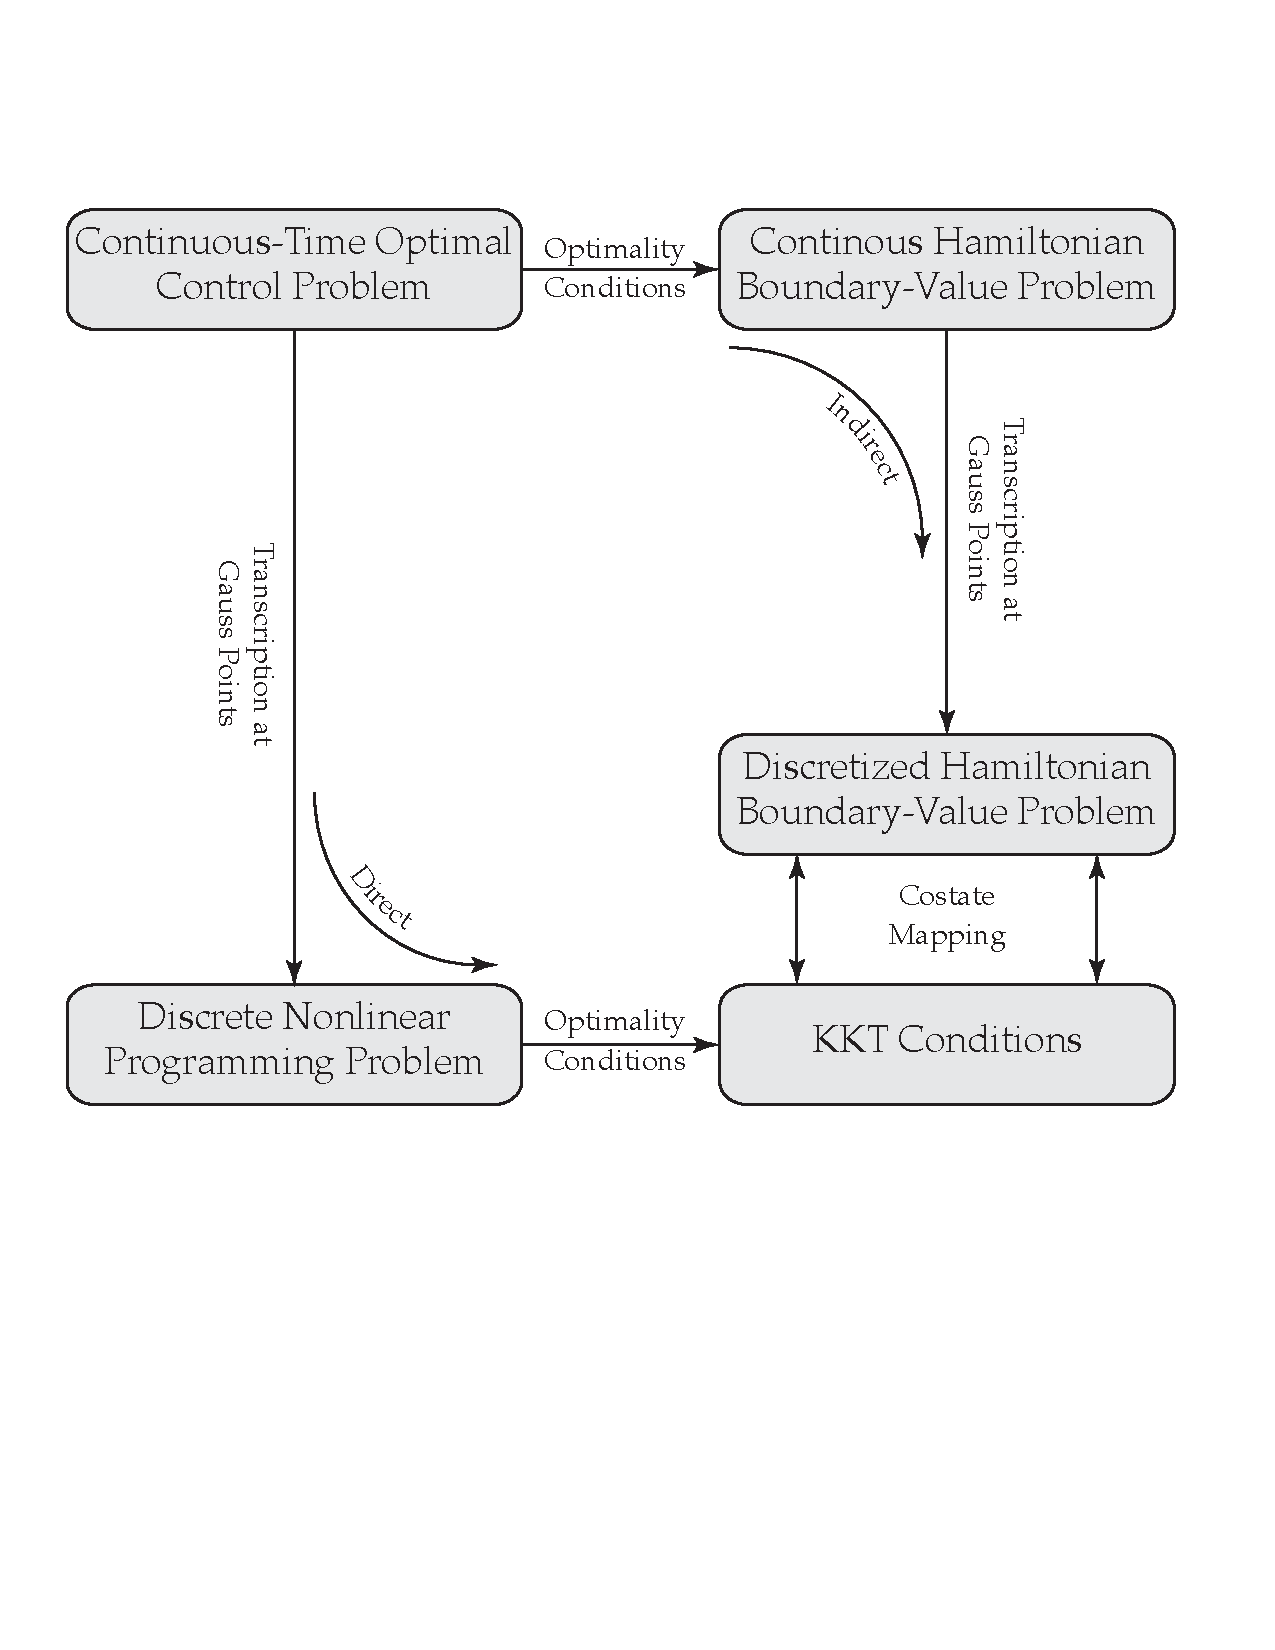
\includegraphics[scale=0.7]{diff_flow.pdf}
  \caption{Equivalence of indirect and direct forms using the Gauss pseudospectral discretization.\label{diff_flow_fig}}
\end{figure}

\section{Computation of Boundary Controls}

It is seen in the GPM that the control is discretized only at the LG points
and is {\em not} disctretized at either the initial or the terminal point.
Consequently, the solution of the NLP defined by Eqs.~(\ref{diff_dis_dyn}),
(\ref{gauss quadrature of xf}), (\ref{diff_dis_cost}), (\ref{diff_dis_bound}),
and (\ref{diff_dis_path}) does not produce values of the controls at the
boundaries.  The ability to obtain accurate initial and terminal controls can
be important in many applications, particularly in guidance where real-time
computation of the initial control is of vital interest.

At first glance, it may seem that the lack of control information at the
boundaries can be overcome simply via extrapolation of the control at the LG
points.  However, multiple reasons exist as to why this is not the best
approach.  First, no particular functional form for the control is assumed in
the GPM discretization.  As a result, the best function to use for
extrapolation is ambiguous.  Seccond, any reasonable extrapolation of the
control (\eg linear, quadratic, cubic, or spline) may violate a path
constraint which, in general, will render the extrapolated control infeasible.
Third, even if the extrapolated control is feasible, it will not satisfy the
required optimality conditions at the boundaries (\ie the control will be
suboptimal with respect to the NLP).  Consequently, it is both practical and
most rigorous to develop a systematic procedure to compute the boundary
controls.  We now show how to compute the boundary controls from the primal
and dual solutions of the NLP arising from the Gauss pseudospectral method.
It is noted that the algorithm described in this section is taken from
\citeasnoun{Huntington5}

Because the approach for computing the initial and terminal control is
identical, we focus on the computation of the initial control.  First,
recalling the augmented Hamiltonian,  $\tilde{\cal{H}}_a$, for the
continuous-time optimal control problem, we have
\begin{equation}\label{augmented Hamiltonian continuous}
  \tilde{\cal H}_a(\textbf{x},\textbf{u},\boldsymbol{\lambda},\boldsymbol{\mu})
  \equiv g + \boldsymbol{\lambda}^T\textbf{f} -
  \boldsymbol{\mu}^T\textbf{C}
\end{equation}
where shorthand notation is used.  Now recall that, from the minimum principle
of Pontryagin, at  every instant of time the optimal control is the control
$\bfu^*(\tau)\in{\cal U}$ that satisfies the condition
\begin{equation}\label{minimum principle}
  \tilde{\cal H}_a(\textbf{x}^*,\textbf{u}^*,\boldsymbol{\lambda}^*,\boldsymbol{\mu}^*)
  \leq
  \tilde{\cal H}_a(\textbf{x}^*,\textbf{u},\boldsymbol{\lambda}^*,\boldsymbol{\mu}^*)
\end{equation}
where ${\cal U}$ is the feasible control set.  Consequently, for a
given instant of time $\tau$ where $\textbf{x}^*(\tau)$, $\boldsymbol{\lambda}^*(\tau)$,
and $\boldsymbol{\mu}^*(\tau)$ are known, Eq.~(\ref{minimum principle}) is a
constrained optimization problem in the
$\textbf{u}(\tau)\in\mathbb{R}^m$.  In order to solve this
constrained optimization problem at the {\em initial}
time, it is necessary to know $\textbf{x}^*(\tau_0)$,
$\boldsymbol{\lambda}^*(\tau_0)$, and $\boldsymbol{\mu}^*(\tau_0)$.

Consider now the information that can be obtained by solving the NLP
associated with the GPM.  In particular, the primal solution to the NLP
produces $\textbf{X}(\tau_0)$ while the dual solution to the NLP can be
manipulated algebraically to obtain the initial costate, $\boldsymbol{\Lambda}^*(\tau_0)$.
However, because the NLP does not evaluate that path constraint at the boundaries, there is no associated Lagrange multiplier $\tilde{\boldsymbol{\mu}}(\tau_0)$.  This apparent impediment can be overcome by
applying the minimum principle in a manner somewhat different from that given
in Eq.~(\ref{minimum principle}).  In particular, suppose we let
${\cal H}$ be the {\em Hamiltonian} (not the augmented Hamiltonian), where
${\cal H}$ is defined as
\begin{equation}\label{Hamiltonian continuous}
  {\cal H}(\textbf{x},\textbf{u},\boldsymbol{\lambda})
  \equiv g + \boldsymbol{\lambda}^T\textbf{f}
\end{equation}
It is seen in Eq.~(\ref{Hamiltonian continuous}) that the term
involving the path constraint is not included.  The path constraint is instead incorporated into the feasible
control set.  In particular, suppose we let
${\cal V}_0$
\begin{equation}
  {\cal V}_0 = {\cal U} \bigcap {\cal C}_0
\end{equation}
where ${\cal V}_0$ is the intersection of the original set of
feasible controls at time $\tau_0$, denoted ${\cal U}$, with the set of all
controls at time $\tau_0$ that satisfy the inequality constraint of Eq.~(\ref{diff_dis_path}), denoted ${\cal C}_0$.
Then, using the values of $\textbf{X}(\tau_0)$ and
$\boldsymbol{\Lambda}(\tau_0)$, the following modified optimization
problem in $m$ variables $\textbf{U}(\tau_0)\in\mathbb{R}^m$ can be
solved to obtain the initial control, $\textbf{U}(\tau_0)$:
\begin{equation}\label{modified minimum principle}
  \begin{array}{cr}
    \displaystyle\textrm{minimize} &  {\cal
    H}(\textbf{X}(t_0),\textbf{U}(\tau_0),\boldsymbol{\Lambda}(\tau_0),\tau_0;t_0,t_f) \\
    {\textbf{U}(\tau_0)\in{\cal V}_0}
  \end{array}
\end{equation}
It is noted that, because ${\cal V}_0$ is restricted by the
inequality path constraint at $\tau_0$, the solution of $\textbf{U}(\tau_0)$ is
equivalent to the solution of the following problem:
\begin{equation}\label{modified minimum principle 2}
  \begin{array}{rl}
    \displaystyle\textrm{minimize} &  {\cal
    H}(\textbf{X}(\tau_0),\textbf{U}(\tau_0),\boldsymbol{\Lambda}(\tau_0),\tau_0;t_0,t_f) \\
    {\textbf{U}(\tau_0)\in{\cal U}} \\
    \textrm{subject to} \\
    & \textbf{C}(\textbf{X}(\tau_0),\textbf{U}(\tau_0),\tau_0;t_0,t_f) \leq \textbf{0}
  \end{array}
\end{equation}
Interestingly, if the constraint is {\em active}, then the initial path constraint multiplier,
$\tilde{\boldsymbol{\mu}}(\tau_0)$, will also be determined by the minimization
problem of Eq.~(\ref{modified minimum principle 2}).   Finally, as alluded to
above, the control at the terminal time, $\textbf{U}(\tau_f)$, can be obtained by
solving the minimization problem of Eq.~(\ref{modified minimum principle 2})
at $\tau=\tau_f$, \ie
\begin{equation}\label{modified minimum principle 3}
  \begin{array}{rl}
    \displaystyle\textrm{minimize} &  {\cal
    H}(\textbf{X}(\tau_f),\textbf{U}(\tau_f),\boldsymbol{\Lambda}(\tau_f),\tau_f;t_0,t_f) \\
    {\textbf{U}(t_f)\in {\cal U}} \\
    \textrm{subject to} \\
    & \textbf{C}(\textbf{X}(\tau_f),\textbf{U}(\tau_f),\tau_f;t_0,t_f) \leq \textbf{0}
  \end{array}
\end{equation}

\section{Organization of \gpops}

\gpops is organized as follows.  In order to specify the optimal control
problem that is to be solved, the user must write MATLAB functions that
define the following functions in each phase of the problem:
\begin{enumerate}[(1)]
  \item the cost functional
  \item the right-hand side of the differential equations and the path constraints(\ie the differential-algebraic equations)
  \item the boundary conditions (\ie event conditions)
  \item the linkage constraints (\ie how the phases are connected)
\end{enumerate}
In addition, the user must also specify the lower and upper limits on every component of the following quantities:
\begin{enumerate}[(1)]
  \item initial and terminal time of the phase
  \item the state at the following points in time:
    \begin{itemize}
    \item at the beginning of the phase
    \item during the phase
    \item at the end of the phase
    \end{itemize}
  \item the control
  \item the static parameters
  \item the path constraints
  \item the boundary conditions
  \item the phase duration (\ie total length of phase in time)
  \item the linkage constraints (\ie phase-connect conditions)
\end{enumerate}
It is noted that each of the functions must be defined for each phase
of the problem. The remainder of this document is devoted to describing in detail the
MATLAB${}^{\textregistered}$ syntax for describing the optimal control problem and each of the constituent functions.

\section{Notation Used Throughout Remainder of This Manual}

The following notation is adopted for use throughout the remainder of this
manual.  First, all user-specified names will be denoted by {\sl slanted}
characters (not {\em italic}, but {\sl slanted}).  Second, any item denoted by
{\bf boldface characters}  are pre-defined and cannot be changed by the user.
Finally, users with color capability will see the slanted characters in
\slred{red} and will see the boldface characters in \bfblue{blue}.

\chapter{Constructing an Optimal Control Problem in \gpops}

We now proceed to describe the constructs required to specify an
optimal control problem in \gpops.  We note that the key
MATLAB programming elements used in constructing an optimal control
problem in \gpops are {\em structure} and {\em arrays of structures}.

\section{Preliminary Information}

Before proceeding to the details of setting up a problem in
\gpops, the following few preliminary details are useful.  First,
it is important to understand that the \gpops interface is laid
out in {\bf\em phases}.  Using a phase-based approach, it is possible
to describe each segment of the problem independently of the other
segments.  The segments are then {\em linked} together using linkage
conditions (or phase-connect conditions).  Second, it is important to
note that \gpops uses the vectorization capabilities of MATLAB.
In this vein all matrices and vectors in \gpops are oriented
{\bf\em column-wise} for maximum efficiency.  As you read through this
chapter, please keep in mind the column-wise orientation of all
matrices used in \gpops.

\section{Call to \gpops}

The call to \gpops is deceptively simple and is given as follows:
\begin{center}
\noindent{\bf output=gpops(setup)}
\end{center}
The input \slred{setup} is a user-defined structure that contains all
of the information about the optimal control problem to be solved
\footnote{see the detailed description of \slred{setup} in Section
\ref{sect: structure syntax}}.  Finally, the variable
\slred{output} is a structure that contains all of the information
from the original problem {\em plus} the information from the run
itself (\ie the solution)\footnote{See the detailed description of the
  output in Section \ref{sect: output}.}.  The remainder of this
chapter is devoted to describing the fields in the structure \slred{setup}.

\section{Syntax for Setup Structure  \label{sect: structure syntax}}

The user-defined structure \slred{setup} contains required fields and
optional fields.  The required fields in the structure \slred{setup}
are as follows:
\begin{itemize}
\item \bfblue{name}:  a string containing the name of the problem.
\item \bfblue{funcs}:  a structure whose elements contain the names
  of the user-defined function in the problem (see Section \ref{sect:_Func_Names} below).
\item \bfblue{limits}:  an array of structures that contains the
  information about the lower and upper limits on the variables and
  constraints in each phase of the problem (see Section \ref{sect: limits} below).
\item \bfblue{guess}:  an array of structures that contains
  contains a guess of the solution in each phase of the problem (see Section
  \ref{sect: guess} below).
\end{itemize}
The optional fields (and their default values) are as follows:
\begin{itemize}
\item \bfblue{linkages}: an array of structures that contains the
  information about the lower and upper limits of the linkage constraints (see Section \ref{sect: linkages} below).
\item \bfblue{direction}:  a string that indicates the direction of
  the independent variable.  The two possible values for this string
  are ``increasing'' and ``decreasing''. (default=``increasing'')
\item \bfblue{autoscale}: a string that indicates whether or not
  the user would like the optimal control problem to be scaled
  automatically before it is solved. (default=``off'') (see Section \ref{sect:_scaling} below).
\item \bfblue{derivatives}:  a string indicating differentiation method to be used.  Possible values for this   string are ``numerical'', ``complex'', ``automatic'', ``automatic-INTLAB'', ``automatic-MAD'', ``analytic'' (default=``numerical'') (see Section \ref{sect:_derivatives} below).
\item \bfblue{checkDerivatives}: a flag to check user defined analytic derivatives (default=``0'') (see Section \ref{sect:_derivatives} below).
\item \bfblue{maxIterations}:  a positive integer indicating the maximum number of iterations that can be taken by the NLP solver.  
\end{itemize}

\section{Specifying Function Names Used in Optimal Control Problem}\label{sect:_Func_Names}

The syntax for specifying the names of the MATLAB functions is done by
setting the fields in the structure \bfblue{FUNCS} and is given as follows:
\begin{displaymath}
  \begin{array}{lcl}
    \slred{setup}.\bfblue{funcs.cost} & = & \slred{`costfun.m'} \\
    \slred{setup}.\bfblue{funcs.dae} & = & \slred{`daefun.m'} \\
    \slred{setup}.\bfblue{funcs.event} & = & \slred{`eventfun.m'} \\
    \slred{setup}.\bfblue{funcs.link} & = & \slred{`linkfun.m'}
  \end{array}
\end{displaymath}

\begin{shadedframe}

{\noindent}{\bf Example of Specifying Function Names for Use in \gpops}

\vspace{12pt}

{\noindent}Suppose we have a problem whose cost functional,
differential-algebraic equations, event constraints,
and linkage constraints are defined, respectively, via the
\slred{user-defined} functions \slred{mycostfun.m},
\slred{mydaefun.m}, \slred{myeventfun.m}, and
\slred{mylinkfun.m}.  Then the syntax for specifying these functions
for use in \gpops is given as follows:
\begin{verbatim}
setup.funcs.cost    = 'mycostfun';
setup.funcs.dae     = 'mydaefun';
setup.funcs.event   = 'myeventfun';
setup.funcs.link    = 'mylinkfun';
\end{verbatim}

\end{shadedframe}


\section{Syntax for \bfblue{limits} Structure \label{sect: limits}}

Once the user-defined structure \slred{setup} has been defined, the next
step in setting up a problem for use with \gpops is to create
an array of structures of length $P$ (where $P$ is the number of
phases) called \bfblue{limits}, where \bfblue{limits} is a
field of the structure \slred{setup}.  The array of structures
\bfblue{limits} is specified as follows:
\begin{itemize}
  \item \bfblue{limits($p$).nodes}: scalar value specifying the number of nodes in phase $p\in[1,\ldots,P]$.
  \item \bfblue{limits($p$).time.min} and \bfblue{limits($p$).time.max}:
    row vectors, each of length two, that contain the information
    about the lower and upper limits, respectively, on the initial and terminal time in phase
    $p\in[1,\ldots,P]$.  The row vectors
    \bfblue{limits($p$).time.min} and \bfblue{limits($p$).time.max} have the following form:
    \begin{displaymath}
      \begin{array}{lcl}
        \bfblue{limits(\textit{p}).time.min} & = & \left[\begin{array}{cc} t_0^{\textrm{min}} &
            t_f^{\textrm{min}} \end{array} \right] \\
        \bfblue{limits(\textit{p}).time.max} & = & \left[\begin{array}{cc} t_0^{\textrm{max}} &
            t_f^{\textrm{max}} \end{array} \right]
      \end{array}
    \end{displaymath}
  \item \bfblue{limits($p$).state.min} and \bfblue{limits($p$).state.max}:
    matrices, each of size $n_p \times 3$,
    that contain the lower and upper limits, respectively, on the
    state in phase $p\in[1,\ldots,P]$.  Each of the columns of the
    matrices \bfblue{limits($p$).state.min} and
    \bfblue{limits($p$).state.max} are given as follows:
    \begin{itemize}
      \item \bfblue{limits($p$).state.min(:,1)}: a column vector
        containing the lower (upper) limits on the state at the {\em
          start} of phase $p\in[1,\ldots,P]$.
      \item \bfblue{limits($p$).state.min(:,2)}: a column vector
        containing the lower (upper) limits on the state at the {\em
          during} phase $p\in[1,\ldots,P]$.
      \item \bfblue{limits($p$).state.min(:,3)}: a column vector
        containing the lower (upper) limits on the state at the {\em
          terminus} of phase $p\in[1,\ldots,P]$.
      \end{itemize}
      The matrices \bfblue{limits($p$).state.min} and
      \bfblue{limits($p$).state.max} then have the following form:
    \begin{displaymath}
      \begin{array}{lcl}
        \bfblue{limits(\textit{p}).state.min} & = & \left[\begin{array}{ccc} x_{10}^{\textrm{min}}
            & x_{1}^{\textrm{min}} & x_{1f}^{\textrm{min}} \\
            \vdots & \vdots & \vdots \\
            x_{n0}^{\textrm{min}} & x_{n}^{\textrm{min}} & x_{nf}^{\textrm{min}} \\
          \end{array} \right] \\ \\
        \bfblue{limits(\textit{p}).state.max} & = & \left[\begin{array}{ccc} x_{10}^{\textrm{max}}
            & x_{1}^{\textrm{max}} & x_{1f}^{\textrm{max}} \\
            \vdots & \vdots & \vdots \\
            x_{n0}^{\textrm{max}} & x_{n}^{\textrm{max}} & x_{nf}^{\textrm{max}} \\
          \end{array} \right]
      \end{array}
    \end{displaymath}
  \item \bfblue{limits($p$).control.min} and \bfblue{limits($p$).control.max}:  column vectors, each of length
    $m_p$, that contain the lower and upper limits, respectively, on the
    controls in phase $p\in[1,\ldots,P]$.  The column vectors
    \bfblue{limits($p$).control.min} and \bfblue{limits($p$).control.max}
    have the following form:
      \begin{displaymath}
        \begin{array}{lcl}
          \bfblue{limits(\textit{p}).control.min} & = & \left[\begin{array}{c} u_{1}^{\textrm{min}}
              \\ \vdots \\ u_{m}^{\textrm{min}} \end{array} \right] \\ \\
              \bfblue{limits(\textit{p}).control.max} & = & \left[\begin{array}{c} u_{1}^{\textrm{max}}
                  \\ \vdots \\ u_{m}^{\textrm{max}} \end{array} \right]
            \end{array}
        \end{displaymath}
  \item \bfblue{limits($p$).parameter.min} and
    \bfblue{limits($p$).parameter.max}:  column vectors, each of length
    $q_p$, that contain the lower and upper limits, respectively, on the static
    parameters in phase $p\in[1,\ldots,P]$.  The column vectors
    \bfblue{limits($p$).parameter.min} and \bfblue{limits($p$).parameters.max}
    have the following form:
      \begin{displaymath}
        \begin{array}{lcl}
          \bfblue{limits(\textit{p}).parameter.min} & = & \left[\begin{array}{c}
            q_{1}^{\textrm{min}} \\ \vdots \\ q_{q_p}^{\textrm{min}} \\
          \end{array} \right] \\ \\
        \bfblue{limits(\textit{p}).parameter.max} & = & \left[\begin{array}{c}
            q_{1}^{\textrm{max}} \\ \vdots \\ q_{q_p}^{\textrm{max}} \\
          \end{array} \right]
        \end{array}
      \end{displaymath}
  \item \bfblue{limits($p$).path.min} and \bfblue{limits($p$).path.max}: column vectors, each of length
    $r_p$, that contain the lower and upper limits, respectively, on the
    path constraints in phase $p\in[1,\ldots,P]$.   The column vectors
    \bfblue{limits($p$).path.min} and \bfblue{limits($p$).path.max}
    have the following form:
      \begin{displaymath}
        \begin{array}{lcl}
          \bfblue{limits(\textit{p}).path.min} & = & \left[\begin{array}{c}
            c_{1}^{\textrm{min}} \\ \vdots \\ c_{r_p}^{\textrm{min}} \\
          \end{array} \right] \\ \\
        \bfblue{limits(\textit{p}).path.max} & = & \left[\begin{array}{c}
            c_{1}^{\textrm{max}} \\ \vdots \\ c_{r_p}^{\textrm{max}} \\
          \end{array} \right]
        \end{array}
      \end{displaymath}
  \item \bfblue{limits($p$).event.min} and \bfblue{limits($p$).event.max}: column vectors, each of length
    $e_p$, that contain the lower and upper limits on the event
    constraints in phase $p\in[1,\ldots,P]$. The column vectors
    \bfblue{limits($p$).event.min} and \bfblue{limits($p$).event.max}
    have the following form:
    \begin{displaymath}
      \begin{array}{lcl}
        \bfblue{limits(\textit{p}).event.min} & = & \left[\begin{array}{c} \phi_{1}^{\textrm{min}}
            \\ \vdots \\ \phi_{e_p}^{\textrm{min}} \\
          \end{array} \right] \\ \\
        \bfblue{limits(\textit{p}).event.max} & = & \left[\begin{array}{c} \phi_{1}^{\textrm{min}}
            \\ \vdots \\ \phi_{e_p}^{\textrm{min}} \\
          \end{array} \right]
      \end{array}
    \end{displaymath}
  \item \bfblue{limits($p$).duration.min} and
    \bfblue{limits($p$).duration.max}: scalars that contain the lower
    and upper limits on the duration of phase $p\in[1,\ldots,P]$. The
    scalars \bfblue{limits($p$).duration.min} and
    \bfblue{limits($p$).duration.max} have the following form:
    \begin{displaymath}
      \begin{array}{lcl}
        \bfblue{limits(\textit{p}).duration.min} & = & T^{\min} \\
        \bfblue{limits(\textit{p}).duration.max} & = & T^{\max}
      \end{array}
    \end{displaymath}

\end{itemize}
{\noindent}{\bf Note:} any fields that do not apply to a problem (i.e. a problem without event constraints, path constraints, etc.) may be omitted or left as empty matrices (``[]'').

\begin{shadedframe}
{\noindent}{\bf Example of Setting Up a Limits Cell Array}
\vspace{12pt}

As an example of setting up a limits cell array in \gpops,
consider the following two-phase optimal control problem.  In
particular, suppose that {\em phase 1} of the problem has 3 states, 2
controls, 2 path constraints, and 5 event constraints.  Suppose
further that the lower and upper limits on the initial and terminal
time in the first phase are given as
\begin{displaymath}
  \begin{array}{rcccr}
    0 & \leq  & t_0^{(1)} & \leq & 0 \\
    50 & \leq & t_f^{(1)} & \leq & 100
  \end{array}
\end{displaymath}
Next, suppose that the lower and upper limits on the states at the
{\em start} of the first phase are given, respectively, as
\begin{displaymath}
  \begin{array}{rcccr}
    1 & \leq & x_1(t_0^{(1)}) & \leq & 1 \\
    -3 & \leq & x_2(t_0^{(1)}) & \leq & 0 \\
    0 & \leq & x_2(t_0^{(1)}) & \leq & 5
  \end{array}
\end{displaymath}
Similarly, suppose that the lower and upper limits on the states
{\em during}  the first phase are given, respectively, as
\begin{displaymath}
  \begin{array}{rcccr}
    1 & \leq & x_1(t^{(1)}) & \leq & 10 \\
    -50 & \leq & x_2(t^{(1)}) & \leq & 50 \\
    -20 & \leq & x_2(t^{(1)}) & \leq & 20
  \end{array}
\end{displaymath}
Finally, suppose that the lower and upper limits on the states at the
{\em terminus} of the first phase are given, respectively, as
\begin{displaymath}
  \begin{array}{rcccr}
    5 & \leq & x_1(t_f^{(1)}) & \leq & 7 \\
    2 & \leq & x_2(t_f^{(1)}) & \leq & 2.5 \\
    -\pi & \leq & x_2(t_f^{(1)}) & \leq & \pi
  \end{array}
\end{displaymath}
Next, suppose that the lower and upper limits on the controls
{\em during} the first phase are given, respectively, as
\begin{displaymath}
  \begin{array}{rcccr}
    -50 & \leq & u_1(t^{(1)}) & \leq & 50 \\
    -100 & \leq & u_2(t^{(1)})& \leq & 100
  \end{array}
\end{displaymath}
Next, suppose that the lower and upper limits on the path constraints
{\em during} the first phase are given, respectively, as
\begin{displaymath}
  \begin{array}{rcccr}
    -10 & \leq & p_1(t^{(1)}) & \leq & 10 \\
     1 & \leq & p_2(t^{(1)})& \leq & 1
  \end{array}
\end{displaymath}
Next, suppose that the lower and upper limits on the event constraints
of the first phase are given, respectively, as
\begin{displaymath}
  \begin{array}{rcccr}
    0 & \leq & \phi_1^{(1)} & \leq & 1 \\
     -2 & \leq & \phi_2^{(1)} & \leq & 4 \\
    8 & \leq & \phi_3^{(1)} & \leq & 20 \\
    3 & \leq & \phi_4^{(1)} & \leq & 3 \\
    10 & \leq & \phi_5^{(1)} & \leq & 10
  \end{array}
\end{displaymath}
In a similar manner, suppose that {\em phase 2} of the problem contains the
following information:  4 states, 3 controls, 1 path constraint, and 4
event constraints.  Also, suppose now that the lower and upper limits
on the initial and terminal time in the first phase are given,
respectively, as
\begin{displaymath}
  \begin{array}{rcccr}
    50 & \leq  & t_0^{(2)} & \leq & 100 \\
    100 & \leq & t_f^{(2)} & \leq & 200
  \end{array}
\end{displaymath}
Next, suppose that the lower and upper limits on the states at the
{\em start} of the second phase are given, respectively, as
\begin{displaymath}
  \begin{array}{rcccr}
     3 & \leq & x_1(t_0^{(2)}) & \leq & 3 \\
    -10 & \leq & x_2(t_0^{(2)}) & \leq & 4 \\
    7 & \leq & x_3(t_0^{(2)}) & \leq & 18 \\
   25 & \leq & x_4(t_0^{(2)}) & \leq & 75
  \end{array}
\end{displaymath}
Similarly, suppose that the lower and upper limits on the states
{\em during} the second phase are given, respectively, as
\begin{displaymath}
  \begin{array}{rcccr}
    -200 & \leq & x_1(t^{(2)}) & \leq & 200 \\
    -50 & \leq & x_2(t^{(2)}) & \leq & 50 \\
    -20 & \leq & x_3(t^{(2)}) & \leq & 20 \\
    -80 & \leq & x_4(t^{(2)}) & \leq & 80
  \end{array}
\end{displaymath}
Finally, suppose that the lower and upper limits on the states at the
{\em terminus} of the second phase are given, respectively, as
\begin{displaymath}
  \begin{array}{rcccr}
    12 & \leq & x_1(t_f^{(2)}) & \leq & 12 \\
    -60 & \leq & x_2(t_f^{(2)}) & \leq & 30 \\
    -90 & \leq & x_3(t_f^{(2)}) & \leq & 10 \\
   100 & \leq & x_4(t_f^{(2)}) & \leq & 500
  \end{array}
\end{displaymath}
Next, suppose that the lower and upper limits on the controls
{\em during} the second phase are given, respectively, as
\begin{displaymath}
  \begin{array}{rcccr}
    -90 & \leq & u_1(t^{(2)}) & \leq & 90 \\
    -120 & \leq & u_2(t^{(2)})& \leq & 120
  \end{array}
\end{displaymath}
Next, suppose that the lower and upper limits on the path constraints
{\em during} the second phase are given, respectively, as
\begin{displaymath}
  \begin{array}{rcccr}
    -10 & \leq & p_1(t^{(2)}) & \leq & 10 \\
     1 & \leq & p_2(t^{(2)})& \leq & 1
  \end{array}
\end{displaymath}
Finally, suppose that the lower and upper limits on the events
constraints of the second phase phase are given, respectively, as
\begin{displaymath}
  \begin{array}{rcccr}
    0 & \leq & \phi_1^{(2)}  & \leq & 1 \\
     -2 & \leq & \phi_2^{(2)} & \leq & 4 \\
    8 & \leq & \phi_3^{(2)} & \leq & 20 \\
    3 & \leq & \phi_4^{(2)} & \leq & 3
  \end{array}
\end{displaymath}
Then a MATLAB code that would generate the above specification is
given as follows:
\begin{verbatim}

iphase = 1; % Set the phase number to 1
limits(iphase).nodes = 10;
limits(iphase).time.min = [0 50];
limits(iphase).time.max = [0 100];
limits(iphase).state.min = [1 1 5; -3 -50 2; 0 -20 -pi];
limits(iphase).state.max = [1 10  7; 0  50 2.5; 5 20 pi];
limits(iphase).control.min = [-50; -100];
limits(iphase).control.max = [ 50;  100];
limits(iphase).parameter.min = [];
limits(iphase).parameter.max = [];
limits(iphase).path.min = [-10; 1];
limits(iphase).path.max = [10; 1];
limits(iphase).event.min = [0; -2; 8; 3; 10];
limits(iphase).event.max = [1; 4; 20; 3; 10];

iphase = 2; % Set the phase number to 2
limits(iphase).nodes = 10;
limits(iphase).time.min = [50 100];
limits(iphase).time.max = [100 200];
limits(iphase).state.min = [3 -200 12; -10 -50 -60; 7 -20 -90; 25 -80 100];
limits(iphase).state.max = [3 200 12; 4 50 30; 18 20 10; 75 80 500];
limits(iphase).control.min = [-90; -120];
limits(iphase).control.max = [ 90;  120];
limits(iphase).parameter.min = [];
limits(iphase).parameter.max = [];
limits(iphase).path.min = [-10; 10];
limits(iphase).path.max = [1; 1];
limits(iphase).event.min = [0; -2; 8; 3];
limits(iphase).event.max = [1; 4; 20; 3];

setup.limits = limits;

\end{verbatim}
\end{shadedframe}
{\noindent}{\bf Note:}  in order to make the coding easier, we have
introduced the auxiliary integer variable{\bf iphase} so that the user
can more easily reuse code from phase to phase.

\section{Syntax for \bfblue{linkages} Array of Structures \label{sect: linkages}}

Another required field in the structure \slred{setup} is an array of
structures called \bfblue{linkages} that defines the way that the
phases are to be linked.  If there is only one phase in the problem, then
\slred{setup}.\bfblue{linkages} may be set to ``[]''.  If the problem
contains more than a single phase, then \bfblue{linkages} is an array
of structures of length $L$ (where $L$ is the number of pairs of phases
to be linked).  The array of structures \bfblue{linkages} is specified
as follows:
\begin{itemize}
\item \bfblue{linkages($s$).min}: a column vector of length $l_s$
  containing the lower limits on the $s^{th}$ pair of linkages.
\item \bfblue{linkages($s$).max}: a column vector of length $l_s$
  containing the upper limits on the $s^{th}$ pair of linkages.
\item \bfblue{linkages($s$).left.phase}: an integer containing the
  ``left'' phase in the pair of phases to be connected
\item \bfblue{linkages($s$).right.phase}: an integer containing the
  ``right'' phase in the pair of phases to be connected
\end{itemize}
Note that we use the terminology ``left'' and ``right'' in the sense
of viewing a graph of the trajectory on a page where time is
increasing to the right.  Thus, the ``left'' phase corresponds to the
terminus of a phase while the ``right'' phase corresponds to the
start of a phase.

\section{Syntax of Each Function in Optimal Control Problem}

Now that we know {\em which} functions \gpops will use, the next step is to
discuss the syntax of each of these functions.  In general, the syntax for
each function will differ because the quantities being evaluated are different
in nature.  In this section we will explain the syntax of each function.

\subsection{Syntax of Function Used to Evaluate Cost}\label{sect:_Cost_syntax}

The syntax used to evaluate a user-defined cost functional is given as follows:
\begin{center}
\noindent{\bf function [Mayer,Lagrange]=mycostfun(solcost);}
\end{center}
{\noindent}where \slred{mycostfun.m} is the name of the MATLAB function,
\slred{solcost} is the input to the function, and
\slred{Mayer} and \slred{Lagrange} are the outputs.  The input
\slred{solcost} is a structure while the outputs
\slred{Mayer} and \slred{Lagrange} are the endpoint cost and the
integrand of the integrated cost, respectively.  The input structure
\slred{solcost} has the following fields (note that $N$=number of LG points which are on the interior of the time interval):
\begin{itemize}
  \item \slred{solcost}.\bfblue{phase}:  the phase number
  \item \slred{solcost}.\bfblue{initial.time}:  the initial time in phase \slred{solcost}.\bfblue{phase}
  \item \slred{solcost}.\bfblue{initial.state}:  the initial state in phase \slred{solcost}.\bfblue{phase}
  \item \slred{solcost}.\bfblue{terminal.time}:  the terminal time in phase \slred{solcost}.\bfblue{phase}
  \item \slred{solcost}.\bfblue{terminal.state}:  the terminal state in phase \slred{solcost}.\bfblue{phase}
  \item \slred{solcost}.\bfblue{time}:  a column vector of length $N$ that
    contains the time (excluding the initial and terminal points) in
    phase \slred{solcost}.\bfblue{phase}
  \item \slred{solcost}.\bfblue{state}:  a matrix of size $N\times n$ (where $n$
    is the number of states) that contains the values of the state (excluding the initial and
    terminal points) in phase \slred{solcost}.\bfblue{phase}
  \item \slred{solcost}.\bfblue{control}:  a matrix of size $N\times m$ (where $m$
    is the number of controls) that contains the values of the control (excluding the initial and
    terminal points) in phase \slred{solcost}.\bfblue{phase}
  \item \slred{solcost}.\bfblue{parameter}:  a column vector of length $q$ that contains the values of the static parameters in phase \slred{solcost}.\bfblue{phase}
\end{itemize}
Finally, the outputs of \slred{mycostfun} are as follows:
\begin{itemize}
  \item \slred{Mayer}: a {\em scalar}, \ie size $1\times 1$
  \item \slred{Lagrange}: a {\em column} vector of size $N\times 1$
\end{itemize}

\subsection{Warning About Outputs to Cost Function}

For many optimal control problems the output \slred{Lagrange} in the
user-defined cost function \slred{mycostfun} is {\bf\em zero}.  As such, it is
appealing to set \slred{Lagrange} to zero by the MATLAB command
\begin{equation}
  \textrm{Lagrange=0;}
\end{equation}
However, {\bf\em the integrand cannot be set to a scalar value!}.  Instead,
the integrand {\bf\em must} be set to a {\bf\em column vector of zeros!}.  The
way to set the integrand to zero and that {\bf\em will work in all cases} (\ie
numerical or automatic differentiation) is as follows:
\begin{equation}\label{integrand correct syntax zero}
  \boxed{
    \textrm{Lagrange=zeros(size(\slred{solcost}.\bfblue{time});}
  }
\end{equation}
The user is urged to use the syntax of Eq.~(\ref{integrand correct syntax zero})
whenever the integrand is identically zero.

\begin{shadedframe}
{\noindent}{\bf Example of a Cost Functional}
\vspace{12pt}

Suppose we have a two-phase optimal control problem that uses a cost
functional named ``mycostfun.m''.  Suppose further that the dimension of the
state in each phase is 2 while the dimension of the control in each phase is
2.  Also, suppose that the endpoint and integrand cost in phase 1 are
given, respectively, as
\begin{displaymath}
  \begin{array}{lcl}
    \Phi^{(1)}(\bfx^{(1)}(t_0),t_0^{(1)},\bfx^{(1)}(t_f),t_f^{(1)}) & = & \bfx^T(t_f)\bfS\bfx(t_f) \\
    \mcL^{(1)}(\bfx^{(1)}(t),\bfu^{(1)}(t),t) & = & \bfx^T\bfQ\bfx + \bfu^T\bfR\bfu
  \end{array}
\end{displaymath}
while the endpoint and integrand in phase 2 are given, respectively, as
\begin{displaymath}
  \begin{array}{lcl}
    \Phi^{(2)}(\bfx^{(2)}(t_0^{(2)}),t_0^{(2)},\bfx^{(2)}(t_f^{(2)}),t_f^{(2)}) & = & \bfx^T(t_f)\bfx(t_f) \\
    \mcL^{(2)}(\bfx^{(2)}(t),\bfu^{(2)}(t),t) & = & \bfu^T\bfR\bfu
  \end{array}
\end{displaymath}
Then the syntax of the above cost functional is given as follows:
\begin{verbatim}
function [endpoint,integrand]=mycostfun(solcost);

Q = [5 0; 0 2];
R = [1 0; 0 3];
S = [1 5; 5 1];
iphase = solcost.phase;
t0 = solcost.initial.time;
x0 = solcost.initial.state;
tf = solcost.terminal.time;
xf = solcost.terminal.state;
t  = solcost.time;
x  = solcost.state;
u  = solcost.control;
p  = solcost.parameter;

if iphase==1,
  Mayer  = dot(xf',S*xf');
  Lagrange = dot(x,x*Q',2)+dot(u,u*R',2); % Note transposes
elseif iphase==2,
  Mayer  = dot(xf,xf);
  Lagrange = dot(u,u*R',2); % Note transposes
end;
\end{verbatim}
It is noted in the above function call that the third argument in the
command {\bf dot} takes the dot product across the {\em rows}, thereby
producing a {\em column vector}.
\end{shadedframe}

\subsection{Syntax of Function Used to Evaluate Differential-Algebraic Equations\label{sect:_Dae_syntax}}

The calling syntax used evaluate the right-hand side of a user-defined vector
of differential equations is given as follows:
\begin{center}
  \noindent{\bf function dae=mydaefun(soldae);}
\end{center}
{\noindent}where \slred{mydaefun.m} is the name of the MATLAB function,
\slred{soldae} is the input to the function, and
\slred{dae} is the output (\ie the right-hand side of the
differential equations and the values of the path constraints).  The
input \slred{soldae} is a structure while the output \slred{dae} is a
matrix of size $N \times (n+c)$ where $n$ is the number of
differential equations, $c$ is the number of path constraints, and $N$
is the number of LG points.  The input structure \slred{soldae} has
the following fields:
\begin{itemize}
  \item \slred{soldae}.\bfblue{phase}:  the phase number
  \item \slred{soldae}.\bfblue{time}:  a column vector of length $N$ that
    contains the time (excluding the initial and terminal points) in phase \slred{soldae}.\bfblue{phase}
  \item \slred{soldae}.\bfblue{state}:  a matrix of size $N\times n$ (where $n$
    is the number of states) that contains the values of the state (excluding the initial and
    terminal points) in phase \slred{soldae}.\bfblue{phase}
  \item \slred{soldae}.\bfblue{control}:  a matrix of size $N\times m$ (where $m$
    is the number of controls) that contains the values of the control (excluding the initial and
    terminal points) in phase \slred{soldae}.\bfblue{phase}
  \item \slred{soldae}.\bfblue{parameter}:  a column vector of length $q$ that
    contains the values of the static parameters in phase \slred{soldae}.\bfblue{phase}
\end{itemize}
Finally, the output of \slred{myodefun} are as follows:
\begin{itemize}
  \item \slred{dae}: a {\em matrix} of size $N\times (n+c)$ containing
    the values of the right-hand side of the $n$ differential
    equations and the $c$ path constraints evaluated at the $N$ LG points
\end{itemize}

\begin{shadedframe}
  {\noindent}{\bf Example of a Differential-Algebraic Equation}
\vspace{12pt}

Suppose we have a two-phase optimal control problem that uses a differential
equation function called ``mydaefun.m''.  Suppose further that the dimension
of the state in each phase is 2, the dimension of the control in each
phase is 2.  Furthermore, suppose that there are no path constraints
in phase 1 and one path constraint in phase 2.  Next, suppose that
the differential equations in phase 1 are given as
\begin{displaymath}
  \begin{array}{lcl}
    \dx_1 & = & -x_1^2-x_2^2 + u_1 u_2 \\
    \dx_2 & = & -x_1x_2 + 2(u_1+u_2)
  \end{array}
\end{displaymath}
Also, suppose that the differential equations in phase 2 are given as
\begin{displaymath}
  \begin{array}{lcl}
    \dx_1 & = & \sin(x_1^2+x_2^2) + u_1 u_2^2 \\
    \dx_2 & = & -\sin x_1 \cos x_2 + 2u_1u_2
  \end{array}
\end{displaymath}
Finally, suppose that the path constraint in phase 2 is given as
\begin{displaymath}
  u_1^2+u_2^2 = 1
\end{displaymath}
Then a MATLAB code that will evaluate the above system of
differential-algebraic equations is given as follows:
\begin{verbatim}
function dae = mydaefun(soldae);

iphase = soldae.phase;
t = soldae.time;
x = soldae.state;
u = soldae.control;
p = soldae.parameter;

if iphase==1,
  x1dot = -x(:,1).^2-x(:,2).^2 + u(:,1).*u(:,2);
  x2dot = -x(:,1).*x(:,2) + 2*(u(:,1)+u(:,2));
  path = [];
elseif iphase==2,
  x1dot = sin(x(:,1).^2 + x(:,2).^2) + u(:,1).*u(:,2).^2;
  x2dot = -sin(x(:,1)).*cos(x(:,2))+2*u(:,1).*u(:,2);
  path  = u(:,1).^2+u(:,2).^2;
end;
dae = [x1dot x2dot path];
\end{verbatim}

\end{shadedframe}

\subsection{Syntax of Function Used to Evaluate Event Constraints\label{sect:_Event_syntax}}

The syntax used to evaluate a user-defined vector of event constraints
is given as follows:
\begin{center}
\noindent{\bf function events=myeventfun(solevents,iphase);}
\end{center}
{\noindent}where \slred{myeventfun.m} is the name of the MATLAB function,
\slred{solevents} and \slred{iphase} are the inputs to the function, and
\slred{event} is the output (\ie the value of the event constraints).
The inputs \slred{solevents} and \slred{iphase} are a cell array and
an integer, respectively, while the output \slred{event} is a
{\em column vector} of length $e$ where $e$ is the number of event
constraints.  The input cell array \slred{solevents} has the following elements:
\begin{itemize}
  \item \slred{solevents}.\bfblue{phase}:  the phase number
  \item \slred{solevents}.\bfblue{initial.time}:  the time at the start of the phase
  \item \slred{solevents}.\bfblue{initial.state}:  the state at the start of the phase
  \item \slred{solevents}.\bfblue{terminal.time}:  the time at the terminus of the phase
  \item \slred{solevents}.\bfblue{terminal.state}:  the state at the terminus of the phase
  \item \slred{solevents}.\bfblue{parameter}:  the static parameters in the phase
\end{itemize}

\begin{shadedframe}
{\noindent}{\bf Example of Event Constraints}
\vspace{12pt}

{\noindent}Suppose we have a one-phase optimal control problem that has two
initial event constraints and three terminal event constraints.  Suppose
further that the number of states in the phase is six and that the function
that computes the values of these constraints is called ``myeventfun.m''.
Finally, let the two initial event constraints be given as
\begin{displaymath}
  \begin{array}{lcl}
    \phi_{01} & = & x_1(t_0)^2+x_2(t_0)^2+x_3(t_0)^2 \\
    \phi_{02} & = & x_4(t_0)^2+x_5(t_0)^2+x_6(t_0)^2
  \end{array}
\end{displaymath}
while the three terminal event constraints are given as
\begin{displaymath}
  \begin{array}{lcl}
    \phi_{f1} & = & \sin(x_1(t_f))\cos(x_2(t_f)+x_3(t_f)) \\
    \phi_{f2} & = & \tan(x_4^2(t_f)+x_5^2(t_f)+x_6^2(t_f)) \\
    \phi_{f3} & = & x_4(t_f)+x_5(t_f)+x_6(t_f)
  \end{array}
\end{displaymath}
Then the syntax of the above event function is given as
\begin{verbatim}
function events = myeventfun(solevents);

iphase = solevents.phase;
t0 = solevents.initial.time;
x0 = solevents.initial.state;
tf = solevents.terminal.time;
xf = solevents.terminal.state;

ei1 = dot(x0(1:3),x0(1:3));
ei2 = dot(x0(4:6),x0(4:6));
ef1 = sin(xf(1))*cos(xf(2)+xf(3));
ef2 = tan(dot(xf(4:6),xf(4:6)));
ef3 = xf(4)+xf(5)+xf(6);

events = [ei1;ei2;ef1;ef2;ef3];
\end{verbatim}

\end{shadedframe}

Finally, it is noted that each event constraint need not be a function of
either the initial or the terminal state, but can also be functions that
contain {\em both} the initial and terminal state and/or the initial and
terminal time.  As an example of an event constraint that contains both the
initial and terminal state, consider the following example.

\begin{shadedframe}
{\noindent}{\bf Example of Event Constraint Containing Both Initial and Terminal State}
\vspace{12pt}

{\noindent}Suppose we have a one-phase optimal control problem that contains
only a single state.  Furthermore, suppose that the problem contains a single
event constraint on the {\em difference} between the terminal value of the
state and the initial value of the state.  Finally, suppose that the function
that computes the values of these constraints is called ``myeventfun.m''.
Then the event constraint is evaluated as
\begin{displaymath}
  \phi = x(t_f)-x(t_0)
\end{displaymath}
Then the syntax of the above event function is given as
\begin{verbatim}
function events = myeventfun(solevents);

t0 = solevents.initial.time;
x0 = solevents.initial.state;
tf = solevents.terminal.time;
xf = solevents.terminal.state;

events = xf-x0;
\end{verbatim}

\end{shadedframe}

\subsection{Syntax of Function Used to Evaluate Linkage Constraints\label{sect:_Link_syntax}}

The syntax used to define the user defined vector of linkage
constraints between two phases is given as follows:
\begin{center}
\noindent{\bf function links=mylinkfun(sollink);}
\end{center}
{\noindent}where \slred{mylinkfun.m} is the name of the MATLAB function,
\slred{sollink} is the input to the function, and \slred{links} is the output (\ie the value of the linkage
constraints).  The input \slred{sollink} is a structure while the output \slred{links} is a {\em column vector} of length $l$,
where $l$ is the number of event constraints. The input structure \slred{sollink} has the following fields:
\begin{itemize}
  \item \slred{sollink}.\bfblue{left.phase}:  the left phase of the
    pair of phases to be linked
  \item \slred{sollink}.\bfblue{right.phase}:  the right phase of the pair of phases to be linked
  \item \slred{sollink}.\bfblue{left.state}: the state at the terminus of phase \slred{sollink}.\bfblue{left.phase}
  \item \slred{sollink}.\bfblue{right.state}: the state at the start of phase \slred{sollink}.\bfblue{right.phase}
  \item \slred{sollink}.\bfblue{left.parameter}: the static parameters in phase \slred{sollink}.\bfblue{left.phase}
  \item \slred{sollink}.\bfblue{right.state}: the static parameters in phase \slred{sollink}.\bfblue{right.phase}
\end{itemize}
The terms {\em left} and {\em right} are conventions adopted to help
the user orient the phases on a page from left to right.

\begin{shadedframe}
{\noindent}{\bf Example of Linkage Constraint}
\vspace{12pt}

{\noindent}Suppose we have a multiple phase optimal control problem with a simple link between the phases, i.e. the state of the end of the phase is equal to the state at the beginning of the next phase.  \begin{displaymath}
\bfP = x^l(t_f) - x^r(t_0)
\end{displaymath}
Then the syntax of the above linkage is given as
\begin{verbatim}
function links = mylinkagefun(sollink);

left_phase = sollink.left.phase;
right_phase = sollink.right.phase;
xf_left = sollink.left.state;
p_left  = sollink.left.parameter;
x0_left = sollink.right.phase;
p_left  = sollink.right.parameter;

links = xf_left - x0_right;
\end{verbatim}
\end{shadedframe}

\section{Specifying an Initial Guess of The Solution \label{sect: guess}}

The field \bfblue{guess} of the user-defined structure \slred{setup}
contains the initial guess for the problem.  The field
\bfblue{guess} is an array of structures of length $P$ (where $P$ is the
number of phases in the problem).  The $p^{th}$ element of the array
of structures \bfblue{guess} contains the initial guess of the problem in phase
$p\in[1,\ldots,P]$.  The fields of each element of array of structures
\bfblue{guess} are given as follows:
\begin{itemize}
\item \bfblue{guess(\textit{p}).time}:  a {\em column} vector of
  length $s$ where $s$ is the number of time points used in the guess
\item \bfblue{guess(\textit{p}).state}:  a matrix of size $s \times n$
  where $s$ is the number of time points and $n$ is the number of
  states in the phase
\item \bfblue{guess(\textit{p}).control}:  a matrix of size $s \times m$
  where $s$ is the number of time points and $m$ is the number of controls in the phase
\item \bfblue{guess(\textit{p}).parameter}:  a column vector of length $q$
  where $q$ is the number of static parameters in the phase
\end{itemize}
It is noted that the element \bfblue{guess(\textit{p}).time} must be
monotonic and in the same direction as that specified by the field
\bfblue{direction} of the structure \slred{setup}.
Schematically, in each phase of the problem the guess for the time,
states, controls, and parameters is structured as follows:
\begin{displaymath}
  \begin{array}{lcl}
    \bfblue{guess(\textit{p}).time} & = &
    \left[\begin{array}{c} t_0 \\ t_1 \\ t_2 \\ \cdots \\
        t_{s} \end{array} \right] \\ \\
    \bfblue{guess(\textit{p}).state} & = &
    \left[\begin{array}{cccc} x_{10} & x_{20} & \cdots & x_{n0} \\
        x_{11} & x_{21} & \cdots & x_{n1} \\
        \vdots & \vdots & \vdots & \vdots \\
        x_{1s} & x_{2s} & \cdots & x_{ns}
        \end{array} \right] \\ \\
    \bfblue{guess(\textit{p}).control} & = &
    \left[\begin{array}{cccc} u_{10} & x_{20} & \cdots & x_{m0} \\
        u_{11} & u_{21} & \cdots & x_{m1} \\
        \vdots & \vdots & \vdots & \vdots \\
        u_{1s} & u_{2s} & \cdots & u_{ms}
        \end{array}
      \right] \\ \\
    \bfblue{guess(\textit{p}).parameter} & = &
    \left[\begin{array}{c} q_1 \\ q_2 \\ \vdots \\ q_q \end{array} \right]
  \end{array}
\end{displaymath}
\begin{shadedframe}

{\noindent}{\bf Example of Specifying an Initial Guess}

\vspace{12pt}
Suppose we have a two-phase problem that has three states and two controls in
phase 1 while it has two states and one control in phase 2.  Furthermore,
suppose that we choose five time points for the guess in phase 1 while we
choose 3 time points for the guess in phase 2.  A MATLAB code that would
create such an initial guess is given below.
\begin{verbatim}

iphase = 1;
guess(iphase).time  = [0; 1; 3; 5; 7];
guess(iphase).state(:,1) = [1.27; 3.1; 5.8; 9.6; -13.7272];
guess(iphase).state(:,2) = [-4.2; -9.6; 8.5; 25.73; 100.00];
guess(iphase).state(:,3) = [18.727; 1.827; 25.272; -14.272; 26.84];
guess(iphase).control(:,1) = [8.4; -13.7; -26.5; 19; 87];
guess(iphase).control(:,2) = [-1.2; 5.8; -3.77; 14; 19.787];
guess(iphase).parameter = [];

iphase = 2;
guess(iphase).time = [7; 7.5; 8];
guess(iphase).state(:,1) = [0.5; 1.5; 8];
guess(iphase).state(:,2) = [-0.5; -2.5; 19];
guess(iphase).control(:,1) = [8.4; -13.7; -26.5; 19; 87];
guess(iphase).parameter = [];

setup.guess = guess;

\end{verbatim}
\end{shadedframe}
It is noted again that, for the above example, auxiliary integer
variables were used to minimize the cumbersomeness of coding and to
minimize the chance of error.

\section{Scaling of Optimal Control Problem\label{sect:_scaling}}

As with any numerical optimization procedure, the approach employed by
\gpops requires a well-scaled optimal control problem.  In general, it is
recommended that the user scale the problem in accordance with any known large
discrepancies either in the sizes of various quantities (\ie state, control)
or the sizes of the derivatives of such quantities.  While it is beyond the
scope of this user's manual to provide a general procedure for scaling, in an
attempt to reduce the burden on the user an automatic scaling procedure has
been developed for use in \gpops.  This procedure is based on the scaling
algorithm developed in \cite{Betts1}.  In order to invoke the automatic
scaling routine, the user must set the field \bfblue{autoscale} in the
user-defined structure \slred{setup} to the string ``on''.

The automatic scaling procedure operates as follows.  The bounds on the
variables are used to scale all components of the state, control, parameters,
and time to lie between -1 and 1.  As a result, it is essential that the user
provide {\em sensible} bounds on all quantities (\eg do not provide
unreasonably large bounds as this will result in a poorly scaled problem).
Next, the constraints are scaled to make the row norms of the Jacobians of the
respective functions approximately unity.  The automatic scaling procedure is
by no means foolproof, but it has been found in practice to work well on many
problems that otherwise would require scaling by hand.  The advice given here
is to try the automatic scaling procedure, but not to use it for too long if
it is proving to be unsuccessful.

\section{Different Options for Specification of Derivatives\label{sect:_derivatives}}

The user has six choices for the computation of the derivatives of
the objective function gradient and the constraint Jacobian for use
within the NLP solver.  As stated above, the choices for
\bfblue{derivatives} are ``numerical'', ``complex'', ``automatic'', ``automatic-INTLAB'',
``automatic-MAD'', and ``analytic'' and correspond to the following differentiation methods:
\begin{itemize}
\item \slred{setup}.\bfblue{derivatives}=``numerical'':  default
  finite-differencing algorithm within SNOPT is used.
\item \slred{setup}.\bfblue{derivatives}=``complex'': the {\em
    built-in} complex-step differentiation method is used.
\item \slred{setup}.\bfblue{derivatives}=``automatic'', the {\em
    built-in} automatic differentiator is used.
\item \slred{setup}.\bfblue{derivatives}=``automatic-INTLAB'':
  automatic differentiation using the third-party program  {\em
    INTLAB} is used (if the program INTLAB is installed on your computer).
\item \slred{setup}.\bfblue{derivatives}=``automatic-MAD'': Matlab
  Automatic Differentiation (MAD) is used (if the program MAD is
  installed on your computer)
\item \slred{setup}.\bfblue{derivatives}=``analytic'': analytic derivatives
(supplied by the user) are used.
\end{itemize}
It is noted that INTLAB can be obtained from Prof.~Siegfried Rump by
visiting the URL \url{http://www.ti3.tu-harburg.de/rump/intlab/} while
MAD can be obtained for a nominal charge by visiting
\url{www.tomopt.com/}.  Note that the functionality for MAD has been
coded in \gpops however, it is not officially supported and therefore
may not continue to function in future versions of \gpops and/or MAD.
The authors recommend using either the built-in automatic
differentiator or INTLAB if automatic differentiation is desired.

\subsection{Complex-Step Differentiation}

Of the differention methods given above, either the built-in automatic
differentiator or the complex-step differentiator most preferred
because these two methods provide highly accurate derivatives and are
both included as part of the \gpops software (\ie the user
does not have to obtain any third-party software). One drawback with
complex-step differentiation, however, is that certain functions need
to be handled with great care.  In particular, the functions {\bf
  min}, {\bf max}, {\bf abs}, and {\bf dot} need to be redefined for
use in complex-step differentiation (see Ref.~\citeasnoun{Martins1} and the URL
\url{http://mdolab.utias.utoronto.ca/resources/complex-step/complexify.f90}
for details).  Finally, the transpose operator must be replaced with a
dot-transpose (\ie a {\em real transpose}) because the standard
transpose in MATLAB produces a complex conjugate transpose and it is
necessary to maintain a real transpose when computing derivatives via
complex-step differentiation.

\subsection{Analytic Differentiation}
Analytic differentiation has the advantage that it is the fasted and most accurate of the four methods, however, it is by far the most complex for the user to compute, code, and verify.  The derivatives for the objective function gradient and the constraint Jacobian are computed from the user defined analytic derivatives.  These derivatives are supplied as an additional output of the user functions for the cost, dae functions, event constraints, and linkage constraints (if applicable).
The user defined derivatives can be checked relative to a finite-difference approximation by setting the flag \slred{setup}.\bfblue{checkDerivatives} equal to one. Upon execution of \gpops, the derivatives will be computed at the user supplied initial guess using a finite-difference approximation and compared to the analytic derivatives with the results printed to the screen.  It is recommended that the user run the derivative checking algorithm a least one time to verify that the derivatives are correct, however, it should be noted that the algorithm is not guaranteed to find any incorrect derivatives.  The user must take special care to ensure that the analytic derivatives are coded correctly in order to take advantage of the speed and accuracy of analytic differentiation.

\subsubsection{Syntax of Function Used to Evaluate Cost with Derivatives}

The syntax used to evaluate the user-defined cost derivatives is given as follows:
\begin{center}
\noindent{\bf function [Mayer,Lagrange,DerivMayer,DerivLagrange]=mycostfun(solcost);}
\end{center}
See Section \ref{sect:_Cost_syntax} for the definition of the regular inputs/outputs.
The additional outputs of \slred{mycostfun} are as follows:
\begin{itemize}
  \item \slred{DerivMayer}: a {\em row} vector of size $1\times (2n+2+q)$
  \item \slred{DerivLagrange}: a {\em matrix} of size $N\times (n+m+q+1)$
\end{itemize}
where $n$ is the number of states, $m$ is the number of controls, $q$ is the number of parameters, and $N$ is the number of LG points in the phase. The row vector \slred{DerivMayer} defines the partial derivatives of the Mayer cost with respect to the initial state, initial time, final state, final time, and finally the parameters:
\begin{center}
\noindent{\bf DerivMayer = $\left[\displaystyle \pd{\Phi}{\bfx(t_0)}, \quad \pd{\Phi}{t_0}, \quad \pd{\Phi}{\bfx(t_f)}, \quad \pd{\Phi}{t_f}, \quad \pd{\Phi}{p}\right]$}
\end{center}
The matrix \slred{DerivLagrange} defines the partial derivatives of the Lagrange cost with respect to the state, control, parameters, and time at each of the $N$ LG points:
\begin{center}
\noindent{\bf DerivLagrange = $\left[\displaystyle \pd{\mcL}{\bfx}, \quad \pd{\mcL}{\bfu}, \quad \pd{\mcL}{p}, \quad \pd{\mcL}{t}\right]$}
\end{center}
It is important to provide all the derivatives in the correct order {\em even if} they are zero.

\begin{shadedframe}
{\noindent}{\bf Example of a Cost Functional with Derivatives}
\vspace{12pt}

Suppose we have a two-phase optimal control problem that uses a cost
functional named ``mycostfun.m''.  Suppose further that the dimension of the
state in each phase is 2 while the dimension of the control in each phase is
2.  Also, suppose that the endpoint and integrand cost in phase 1 are
given, respectively, as
\begin{displaymath}
  \begin{array}{lcl}
    \Phi^{(1)}(\bfx^{(1)}(t_0),t_0^{(1)},\bfx^{(1)}(t_f),t_f^{(1)}) & = & \bfx^T(t_f)\bfS\bfx(t_f) \\
    \mcL^{(1)}(\bfx^{(1)}(t),\bfu^{(1)}(t),t) & = & \bfx^T\bfQ\bfx + \bfu^T\bfR\bfu
  \end{array}
\end{displaymath}
while the endpoint and integrand in phase 2 are given, respectively, as
\begin{displaymath}
  \begin{array}{lcl}
    \Phi^{(2)}(\bfx^{(2)}(t_0^{(2)}),t_0^{(2)},\bfx^{(2)}(t_f^{(2)}),t_f^{(2)}) & = & \bfx^T(t_f)\bfx(t_f) \\
    \mcL^{(2)}(\bfx^{(2)}(t),\bfu^{(2)}(t),t) & = & \bfu^T\bfR\bfu
  \end{array}
\end{displaymath}
Then the syntax of the above cost functional is given as follows:
\begin{verbatim}
function [Mayer,Lagrange,DerivMayer,DerivLagrange]=mycostfun(solcost,iphase);

Q = [5 0; 0 2];
R = [1 0; 0 3];
S = [1 5; 5 1];
t0 = solcost.initial.time;
x0 = solcost.initial.state;
tf = solcost.terminal.time;
xf = solcost.terminal.state;
t  = solcost.time;
x  = solcost.state;
u  = solcost.control;
p  = solcost.parameter;

if iphase==1,
  Mayer  = dot(xf',S*xf');
  Lagrange = dot(x,x*Q',2)+dot(u,u*R',2); % Note transposes
  DerivMayer = [zeros(1,length(x0)), zeros(1,length(t0)), ...
                xf'*S, zeros(1,length(tf), zeros(1,length(p))];
  DerivLagrange = [x*Q', u*R', ...
                   zeros(length(t),length(p)), zeros(size(t))];
elseif iphase==2,
  Mayer  = dot(xf,xf);
  Lagrange = dot(u,u*R',2); % Note transposes
  DerivMayer = [zeros(1,length(x0)), zeros(1,length(t0)), ...
                xf', zeros(1,length(tf), zeros(1,length(p))];
  DerivLagrange = [zeros(size(x)), u*R', ...
                   zeros(length(t),length(p)), zeros(size(t))];
end;
\end{verbatim}
It is noted in the above function call that the third argument in the
command {\bf dot} takes the dot product across the {\em rows}, thereby
producing a {\em column vector}.

\end{shadedframe}

\subsubsection{Syntax of Function Used to Evaluate Differential-Algebraic Equations with Derivatives}


The calling syntax used evaluate the derivatives of the right-hand side of a user-defined vector
of differential equations is given as follows:
\begin{center}
  \noindent{\bf function [dae,Derivdae]=mydaefun(soldae);}
\end{center}
See Section \ref{sect:_Dae_syntax} for the definition of the regular inputs/outputs.
The additional output of \slred{myodefun} is as follows:
\begin{itemize}
  \item \slred{Derivdae}: a {\em matrix} of size $N(n+c) \times (n+m+q+1)$
\end{itemize}
where $n$ is the number of states, $m$ is the number of controls, $q$ is the number of parameters, $c$ is the number of path constraints, and $N$ is the number of LG points in the phase.  The matrix \slred{Derivdae} defines the partial derivatives of the differential equations and path constraints with respect to the state, control, parameters, and time at each of the $N$ LG points:
\begin{center}
\noindent{\bf Derivdae = $\left[\begin{array}{rrrr}
\displaystyle \pd{\bff_1}{\bfx}, &\quad \displaystyle\pd{\bff_1}{\bfu}, &\quad \displaystyle\pd{\bff_1}{p}, &\quad \displaystyle\pd{\bff_1}{t} \vspace{6pt}\\
 \vdots, &\quad \vdots, &\quad \vdots, &\quad \vdots \vspace{6pt}\\
\displaystyle \pd{\bff_n}{\bfx}, &\quad \displaystyle\pd{\bff_n}{\bfu}, &\quad \displaystyle\pd{\bff_n}{p}, &\quad \displaystyle\pd{\bff_n}{t}\vspace{6pt}\\
\displaystyle \pd{\bfC_1}{\bfx}, &\quad \displaystyle\pd{\bfC_1}{\bfu}, &\quad \displaystyle\pd{\bfC_1}{p}, &\quad \displaystyle\pd{\bfC_1}{t}\vspace{6pt}\\
\vdots, &\quad \vdots, &\quad \vdots, &\quad \vdots\vspace{6pt}\\
\displaystyle \pd{\bfC_r}{\bfx}, &\quad \displaystyle\pd{\bfC_r}{\bfu}, &\quad \displaystyle\pd{\bfC_r}{p}, &\quad \displaystyle\pd{\bfC_r}{t}
\end{array}\right]$}
\end{center}
where $\bff_i$, ($i = 1,\ldots,n$) is the right-hand side of the $i^{th}$ differential equation, and $\bfC_j$, ($j = 1,\ldots,r$) is the $j^{th}$ path constraint. It is important to provide all the derivatives in the correct order {\em even if} they are zero.

\begin{shadedframe}
  {\noindent}{\bf Example of a Differential-Algebraic Equation with Derivatives}
\vspace{12pt}

Suppose we have a two-phase optimal control problem that uses a differential
equation function called ``mydaefun.m''.  Suppose further that the dimension
of the state in each phase is 2, the dimension of the control in each
phase is 2.  Furthermore, suppose that there are no path constraints
in phase 1 and one path constraint in phase 2.  Next, suppose that
the differential equations in phase 1 are given as
\begin{displaymath}
  \begin{array}{lcl}
    \dx_1 & = & -x_1^2-x_2^2 + u_1 u_2 \\
    \dx_2 & = & -x_1x_2 + 2(u_1+u_2)
  \end{array}
\end{displaymath}
Also, suppose that the differential equations in phase 2 are given as
\begin{displaymath}
  \begin{array}{lcl}
    \dx_1 & = & \sin(x_1^2+x_2^2) + u_1 u_2^2 \\
    \dx_2 & = & -\sin x_1 \cos x_2 + 2u_1u_2
  \end{array}
\end{displaymath}
Finally, suppose that the path constraint in phase 2 is given as
\begin{displaymath}
  u_1^2+u_2^2 = 1
\end{displaymath}
Then a MATLAB code that will evaluate the above system of
differential-algebraic equations is given as follows:
\begin{verbatim}
function [dae, Derivdae] = mydaefun(soldae);

iphase = soldae.phase;
t = soldae.time;
x = soldae.state;
u = soldae.control;
p = soldae.parameter;

if iphase==1,
  x1dot = -x(:,1).^2-x(:,2).^2 + u(:,1).*u(:,2);
  x2dot = -x(:,1).*x(:,2) + 2*(u(:,1)+u(:,2));
  path = [];
  df1_dx1 = -2*x(:,1);
  df1_dx2 = -2*x(:,2);
  df1_du1 = u(:,2);
  df1_du2 = u(:,1);
  df2_dx1 = -x(:,2);
  df2_dx2 = -x(:,1);
  df2_du1 = 2*ones(size(t));
  df2_du2 = 2*ones(size(t));
  dpath_dx1 = [];
  dpath_dx2 = [];
  dpath_du1 = [];
  dpath_du2 = [];
  dpath_dp = [];
  dpath_dt = [];
elseif iphase==2,
  x1dot = sin(x(:,1).^2 + x(:,2).^2) + u(:,1).*u(:,2).^2;
  x2dot = -sin(x(:,1)).*cos(x(:,2)) + 2*u(:,1).*u(:,2);
  path  = u(:,1).^2+u(:,2).^2;
  df1_dx1 = 2*x(:,1)*cos(x(:,1).^2 + x(:,2).^2);
  df1_dx2 = 2*x(:,2)*cos(x(:,1).^2 + x(:,2).^2);
  df1_du1 = u(:,2).^2;
  df1_du2 = 2*u(:,1).*u(:,2);
  df2_dx1 = -cos(x(:,1)).*cos(x(:,2));
  df2_dx2 = sin(x(:,1)).*sin(x(:,2));
  df2_du1 = 2*u(:,2);
  df2_du2 = 2*u(:,1);
  dpath_dx1 = zeros(size(x(:,1)));
  dpath_dx2 = zeros(size(x(:,2)));
  dpath_du1 = 2*u(:,1);
  dpath_du2 = 2*u(:,2);
  dpath_dp = zeros(length(t),length(p));
  dpath_dt = zeros(size(t));
end;
df1_dp = zeros(length(t),length(p));
df1_dt = zeros(size(t));
df2_dp = zeros(length(t),length(p));
df2_dt = zeros(size(t));

dae = [x1dot x2dot path];

Derivdae = [df1_dx1,   df1_dx2,   df1_du1,   df1_du2,   df1_dp,   df1_dt; ...
            df2_dx1,   df2_dx2,   df2_du1,   df2_du2,   df2_dp,   df2_dt; ...
          dpath_dx1, dpath_dx2, dpath_du1, dpath_du2, dpath_dp, dpath_dt];
\end{verbatim}
\end{shadedframe}

\subsubsection{Syntax of Function Used to Evaluate Event Constraints with Derivatives}


The syntax used to evaluate the derivative of a user-defined vector of event constraints
is given as follows:
\begin{center}
\noindent{\bf function [events, Derivevents]=myeventfun(solevents);}
\end{center}
See Section \ref{sect:_Event_syntax} for the definition of the regular inputs/outputs.  The additional output of \slred{myeventfun} is as follows:
\begin{itemize}
  \item \slred{Derivevents}: a {\em matrix} of size $e\times (2n+2+q)$
\end{itemize}
where $n$ is the number of states, $q$ is the number of parameters, and $e$ is the number of event constraints in the phase.  The matrix \slred{Derivevents} defines the partial derivatives of each event constraint with respect to the initial state, initial time, final state, final time, and parameters:
\begin{center}
\noindent{\bf Derivevents = $\left[\begin{array}{rrrrr}
\displaystyle \pd{\phi_1}{\bfx(t_0)}, &\quad \displaystyle\pd{\phi_1}{t_0}, &\quad \displaystyle\pd{\phi_1}{\bfx(t_f)}, &\quad \displaystyle\pd{\phi_1}{t_f}, &\quad \displaystyle\pd{\phi_1}{p} \vspace{6pt}\\
 \vdots, &\quad \vdots, &\quad \vdots, &\quad \vdots, &\quad \vdots \vspace{6pt}\\
\displaystyle \pd{\phi_e}{\bfx(t_0)}, &\quad \displaystyle\pd{\phi_e}{t_0}, &\quad \displaystyle\pd{\phi_e}{\bfx(t_f)}, &\quad \displaystyle\pd{\phi_e}{t_f}, &\quad \displaystyle\pd{\phi_e}{p}
\end{array}\right]$}
\end{center}
where $\phi_i$, ($i = 1,\ldots,e$) is the $i^{th}$ event constraint. It is important to provide all the derivatives in the correct order {\em even if} they are zero.

\begin{shadedframe}
{\noindent}{\bf Example of Event Constraints with Derivatives}
\vspace{12pt}

{\noindent}Suppose we have a one-phase optimal control problem that has two
initial event constraints and three terminal event constraints.  Suppose
further that the number of states in the phase is six and that the function
that computes the values of these constraints is called ``myeventfun.m''.
Finally, let the two initial event constraints be given as
\begin{displaymath}
  \begin{array}{lcl}
    \phi_{01} & = & x_1(t_0)^2+x_2(t_0)^2+x_3(t_0)^2 \\
    \phi_{02} & = & x_4(t_0)^2+x_5(t_0)^2+x_6(t_0)^2
  \end{array}
\end{displaymath}
while the three terminal event constraints are given as
\begin{displaymath}
  \begin{array}{lcl}
    \phi_{f1} & = & \sin(x_1(t_f))\cos(x_2(t_f)+x_3(t_f)) \\
    \phi_{f2} & = & \tan(x_4^2(t_f)+x_5^2(t_f)+x_6^2(t_f)) \\
    \phi_{f3} & = & x_4(t_f)+x_5(t_f)+x_6(t_f)
  \end{array}
\end{displaymath}
Then the syntax of the above event function is given as
\begin{verbatim}
function [events, Derivevents] = myeventfun(solevents);

iphase = solevents.phase;
t0 = solevents.initial.time;
x0 = solevents.initial.state;
tf = solevents.terminal.time;
xf = solevents.terminal.state;

ei1 = dot(x0(1:3),x0(1:3));
ei2 = dot(x0(4:6),x0(4:6));
ef1 = sin(xf(1))*cos(xf(2)+xf(3));
ef2 = tan(dot(xf(4:6),xf(4:6)));
ef3 = xf(4)+xf(5)+xf(6);

events = [ei1;ei2;ef1;ef2;ef3];

dei1_dx0 = [2*x0(1:3).' zeros(1,3)];
dei1_dt0 = 0;
dei1_dxf = zeros(1,6);
dei1_dtf = 0;
dei1_dp = [];
dei1_dt = 0;
dei2_dx0 = [zeros(1,3), 2*x0(4:6).'];
dei2_dt0 = 0;
dei2_dxf = zeros(1,6);
dei2_dtf = 0;
dei2_dp = [];
def1_dx0 = zeros(1,6);
def1_dt0 = 0;
def1_dxf = [cos(xf(1))*cos(xf(2)+xf(3)), -sin(xf(1))*sin(xf(2)+xf(3)), ...
           -sin(xf(1))*sin(xf(2)+xf(3)), zeros(1,3)];
def1_dtf = 0;
def1_dp = [];
def2_dx0 = zeros(1,6);
def2_dt0 = 0;
def2_dxf = [zeros(1,3), 2*xf(4:6).']/(cos(dot(xf(4:6),xf(4:6))))^2;
def2_dtf = 0;
def2_dp = [];
def3_dx0 = zeros(1,6);
def3_dt0 = 0;
def3_dxf = [zeros(1,3), ones(1,3)];
def3_dtf = 0;
def3_dp = [];

Derivevents = [dei1_dx0, dei1_dt0, dei1_dxf, dei1_dtf, dei1_dp, dei1_dt; ...
               dei2_dx0, dei2_dt0, dei1_dxf, dei2_dtf, dei2_dp, dei2_dt; ...
               def1_dx0, def1_dt0, def1_dxf, def1_dtf, def1_dp, def1_dt; ...
               def2_dx0, def2_dt0, def2_dxf, def2_dtf, def2_dp, def2_dt; ...
               def3_dx0, def3_dt0, def3_dxf, def3_dtf, def3_dp, def3_dt];
\end{verbatim}
\end{shadedframe}

\subsubsection{Syntax of Function Used to Evaluate Linkage Constraints with Derivatives}

The syntax used to define the user defined vector of linkage
constraints between two phases is given as follows:
\begin{center}
\noindent{\bf function [links,Derivlinks]=mylinkfun(sollink);}
\end{center}
See Section \ref{sect:_Link_syntax} for the definition of the regular inputs/outputs. The additional output of \slred{mylinkfun} is as follows:
\begin{itemize}
  \item \slred{Derivlinks}: a {\em matrix} of size $l\times (n^l+q^l+n^r+q^r)$
\end{itemize}
where $l$ is the number of linkages in the constraint, $n^l$ is the number of states in the left phase, $q^l$ is the number of parameters in the left phase, $n^r$ is the number of states in the right phase, and $q^r$ is the number of parameters in the right phase. The matrix \slred{Derivlinks} defines the partial derivatives of each linkage with respect to the left state, left parameters, right state, and right parameters:
\begin{center}
\noindent{\bf Derivlinks = $\left[\begin{array}{rrrr}
\displaystyle \pd{\bfP_1}{\bfx^l(t_f)}, &\quad \displaystyle\pd{\bfP_1}{p^l}, &\quad \displaystyle \pd{\bfP_1}{\bfx^r(t_0)}, &\quad \displaystyle\pd{\bfP_1}{p^r} \vspace{6pt}\\
 \vdots, &\quad \vdots, &\quad \vdots, &\quad \vdots \vspace{6pt}\\
\displaystyle \pd{\bfP_l}{\bfx^l(t_f)}, &\quad \displaystyle\pd{\bfP_l}{p^l}, &\quad \displaystyle \pd{\bfP_l}{\bfx^r(t_0)}, &\quad \displaystyle\pd{\bfP_l}{p^r}
\end{array}\right]$}
\end{center}
where $\bfP_i$, ($i = 1,\ldots,l$) is the $i^{th}$ linkage constraint. It is important to provide all the derivatives in the correct order {\em even if} they are zero.

\begin{shadedframe}
{\noindent}{\bf Example of Linkage Constraint with Derivatives}
\vspace{12pt}

{\noindent}Suppose we have a multiple phase optimal control problem with a simple link between the phases, i.e. the state of the end of the phase is equal to the state at the beginning of the next phase.  \begin{displaymath}
\bfP = x^l(t_f) - x^r(t_0)
\end{displaymath}
Then the syntax of the above linkage is given as
\begin{verbatim}
function [links, Derivlinks] = mylinkagefun(sollink,left_phase,right_phase);

xf_left = sollink.left.state;
p_left  = sollink.left.parameter;
x0_right = sollink.right.state;
p_right  = sollink.right.parameter;

links = xf_left - x0_right;

nlink = length(xf_left); %number of linkages
Derivlinks = [ eye(nlink), zeros(nlink,length(p_left)), ...
              -eye(nlink), zeros(nlink,length(p_right))];
\end{verbatim}
\end{shadedframe}


\section{Output of Execution of \gpops\label{sect: output}}

Upon execution of \gpops, new fields are created in the output structure
\slred{output}.  In particular, upon completion of the execution of
\gpops, the following new fields are created (in addition to the fields
that were created prior to running \gpops on the problem):
\begin{itemize}
  \item \bfblue{solution:}  an array of structures of length $P$
    (where $P$ is the number of phases) containing the solution in each phase
\end{itemize}
The $p^{th}$ element in the array of structures \bfblue{solution}
contains the solution in phase $p\in[1,\ldots,P]$.  The fields of the
array of structures \bfblue{solution} are as follows:
\begin{itemize}
  \item \bfblue{solution(\textit{p}).time:} a column vector of size $M\times 1$
    containing the time at each point along the trajectory (where
    $M=N+2$ is the number of time points and $N$ is the number of LG points)
  \item  \bfblue{solution(\textit{p}).state:}  a matrix of size $M\times n$ such
    that the rows contain the state at the time points along the trajectory
  \item \bfblue{solution(\textit{p}).control:}  a matrix of size $M\times m$ such that the
    rows contain the state at the time points along the trajectory
  \item \bfblue{solution(\textit{p}).parameter:}  a column vector of length $q$
    containing the static parameters
  \item  \bfblue{solution(\textit{p}).costate:}  a matrix of size $M\times n$ such
    that the rows contain the costate at each time point along the trajectory
  \item \bfblue{solution(\textit{p}).pathmult:}  a structure containing the Lagrange
    multipliers of the path constraints
  \item  \bfblue{solution(\textit{p}).Hamiltonian:}  a column vector of size $M\times 1$
    that contains the Hamiltonian at each time point along the trajectory
  \item  \bfblue{solution(\textit{p}).Mayer\_cost:}  The Mayer part of the cost along the trajectory
  \item  \bfblue{solution(\textit{p}).Lagrange\_cost:}  The Lagrange (integrated) cost along the trajectory
\end{itemize}

\section{Useful Information for Debugging a \gpops Problem}

\subsection{Debugging Code when Using Automatic Differentiation}

As stated above, one of the options in \gpops is the use automatic differentiation, either the built-in code, INTLAB or Matlab automatic Differentiation (MAD). As is often the case, the user may want to break
in the various functions to ensure proper coding of the functions.  In
the case where numerical derivatives are used, the variables can be
printed in the MATLAB command window by breaking in the function and
typing the appropriate variable name.  However, when automatic differentiation is being
used, all variables are defined as custom MATLAB objects. The objects are not a
real-valued variable, but is a MATLAB object that contains information
about both the {\em value} of the variables and the {\em derivatives}
of the variables.  If a user wants to obtain the value of a variable, additional commands are necessary.  In the built-in automatic differentiator, the value is obtained using ".value".  For example the value of a variable named ``y'' is obtained by
typing the command ``y.value'' (and not simply by typing ``y'').  When using INTLAB, the value is obtained using ".x" (see INTLAB documentation), i.e. the command ``y.x'' will return the value for variable named "y".  Finally in MAD, the command to get a value is ``getvalue'' (see the TOMLAB/MAD documentation).  For example the value of a variable named ``y'' is obtained by
typing the command ``getvalue(y)''.
The user is urged to keep this in mind when using automatic differentiation to compute
derivatives.


\subsection{Dimensions of Arrays When Debugging \gpops Code}

One aspect of \gpops that may appear confusing when debugging
code pertains to the dimensions of the arrays and the corresponding
time values.  It is important to remember that \gpops uses
collocation at {\em Legendre-Gauss} points.  Because the
Legendre-Gauss points lie on the interior of the time interval of
interest, the dynamics, path constraints, and integrand cost are
computed only at the Legendre-Gauss points.  While this may appear to
be a bit strange, the fundamental point here is that Gaussian
quadrature (which is used in \gpops) only evaluates the functions
at the Legendre-Gauss points.  Do not try to ``fool'' \gpops by
adding the endpoints to the computation of the dynamics, path
constraints, or integrand cost.  If you do this, you will get an error
because the dimensions are incorrect.  For a more complete
mathematical description of the collocation method used in
{\em GPOP}, see either Chapter 1 of this manual or the references
contained in the bibliography at the end of this manual.

\chapter{Examples of Using \gpops}

In this Chapter we provide three complete examples of using \gpops.  For
each example the optimal control problem is first described quantitatively,
then the \gpops code is provided.

\section{Hyper-Sensitive Problem}

\vspace{12pt}

Consider the following optimal control problem.  Minimize the cost functional
\begin{equation}
  J = \frac{1}{2} \int_0^{t_f} \left[ x^2 + u^2 \right] dt
\end{equation}
subject to the dynamic constraint
\begin{equation}
  \dx = -x^3 + u
\end{equation}
and the boundary conditions
\begin{equation}
  \begin{array}{lcl}
    x(0) & = & 1.5 \\
    x(t_f) & = & 1
  \end{array}
\end{equation}
with $t_f=50$.  It is noted that this problem is taken from
\citeasnoun{Rao1}.  The \gpops code that solves this problem
is shown below.  In particular, the following three MATLAB functions
are defined:
\begin{itemize}
  \item hyperSensitiveMain.m: MATLAB m-file (main driver) for problem
  \item hyperSensitiveCost.m: MATLAB function that evaluates the cost functional
  \item hyperSensitiveDae.m:  MATLAB function that evaluates the differential-algebraic equations
\end{itemize}
The beginning and end of each function is labeled by a MATLAB comment.
\footnotesize
\begin{shadedframe}
\verbatiminput{../examples/hyperSensitive/hyperSensitiveMain.m}
\verbatiminput{../examples/hyperSensitive/hyperSensitiveCost.m}
\verbatiminput{../examples/hyperSensitive/hyperSensitiveDae.m}
\end{shadedframe}
\normalsize
The output of the above code from \gpops is summarized in the following three
plots that contain the state ($x$), costate ($\lambda$), and the Hamiltonian
($H$), respectively, for the problem (where $H=L+\lambda f$ where
$L=0.5(x^2+u^2)$ and $f=-x^3+u$).
\begin{figure}[H]
  \centering
  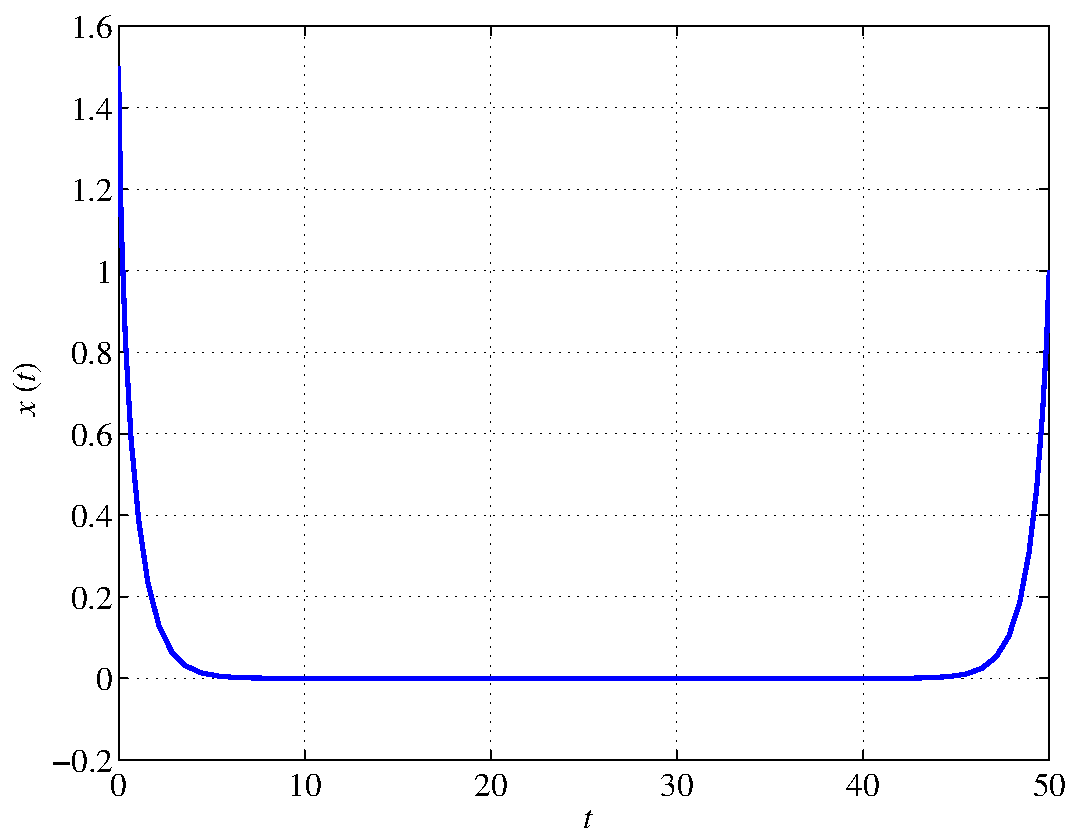
\includegraphics[height=3.5in]{xvst.pdf}
  \caption{$x(t)$ vs.~$t$ for one-dimensional problem.}
\end{figure}
\begin{figure}[H]
  \centering
  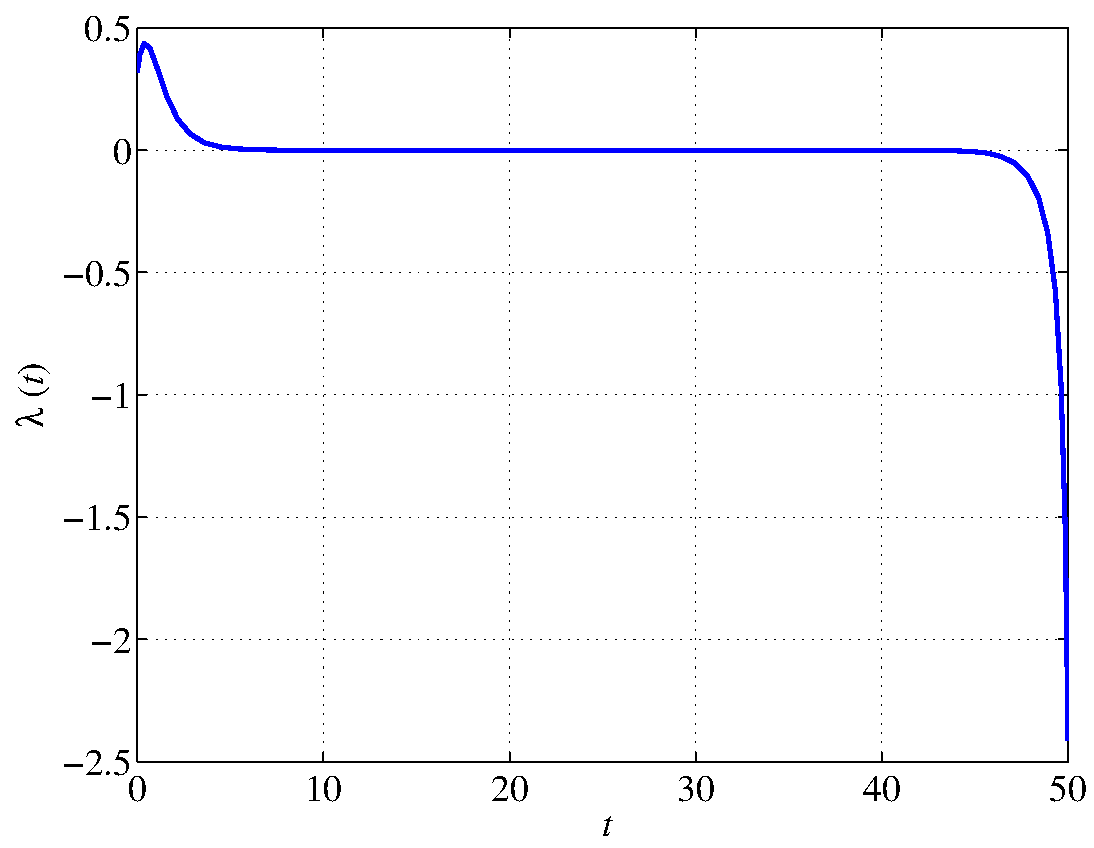
\includegraphics[height=3.5in]{lambdavst.pdf}
  \caption{$\lambda(t)$ vs.~$t$ for one-dimensional problem.}
\end{figure}
\begin{figure}[H]
  \centering
  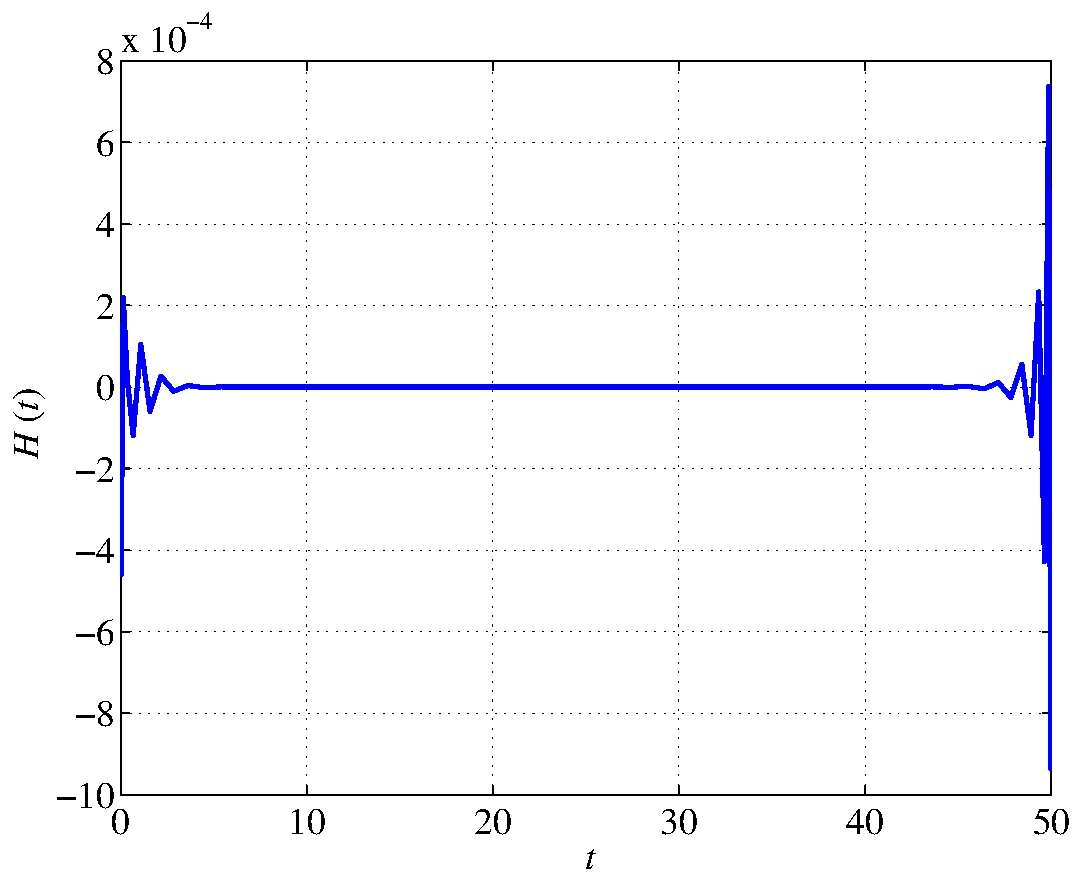
\includegraphics[height=3.5in]{Hamvst_hyper.pdf}
  \caption{$H$ vs.~$t$ for one-dimensional problem.}
\end{figure}

\section{Bryson-Denham Problem}

Consider the following optimal control problem.  Minimize the cost functional
\begin{equation}
  J = x_3(t_f)
\end{equation}
subject to the dynamic constraints
\begin{equation}
  \begin{array}{lcl}
    \dx_1 & = & x_2 \\
    \dx_2 & = & u \\
    \dx_3 & = & \frac{1}{2}u^2
  \end{array}
\end{equation}
the path constraint
\begin{equation}
  0 \leq x_1(t) \leq 1/9
\end{equation}
and the boundary conditions
\begin{equation}
  \begin{array}{lcl}
    x_1(0) & = & 0 \\
    x_2(0) & = & 1 \\
    x_3(0) & = & 0 \\
    x_1(t_f) & = & 0 \\
    x_2(t_f) & = & -1 \\
  \end{array}
\end{equation}
The above problem was originally formulated by Bryson and Denham \cite{Bryson2} and is referred to as the {\em Bryson-Denham} problem.  The
\gpops code that solves the Bryson-Denham problem is shown below.  In
particular, the following four MATLAB files are defined:
\begin{itemize}
  \item brysonDenhamMain.m: MATLAB m-file (main driver) for problem
  \item brysonDenhamCost.m: MATLAB function that evaluates the cost functional
  \item brysonDenhamDae.m: MATLAB function that evaluates the differential-algebraic equation
  \item brysonDenhamEvent.m: MATLAB function that evaluates the event constraints
\end{itemize}
The beginning and end of each function is labeled by a MATLAB
comment. It is noted that while all five boundary conditions are
simple bounds (and are, thus, linear, they are treated as general
event constraints in order to demonstrate the proper use of an event
function.
\footnotesize
\begin{shadedframe}
\verbatiminput{../examples/brysonDenham/brysonDenhamMain.m}
\verbatiminput{../examples/brysonDenham/brysonDenhamCost.m}
\verbatiminput{../examples/brysonDenham/brysonDenhamDae.m}
\end{shadedframe}
\normalsize
The output from \gpops of the Bryson-Denham problem coded
above is summarized in the following plots that contain the components
of the state, the component of the costate, and the control, respectively.
\begin{figure}[H]
  \centering
  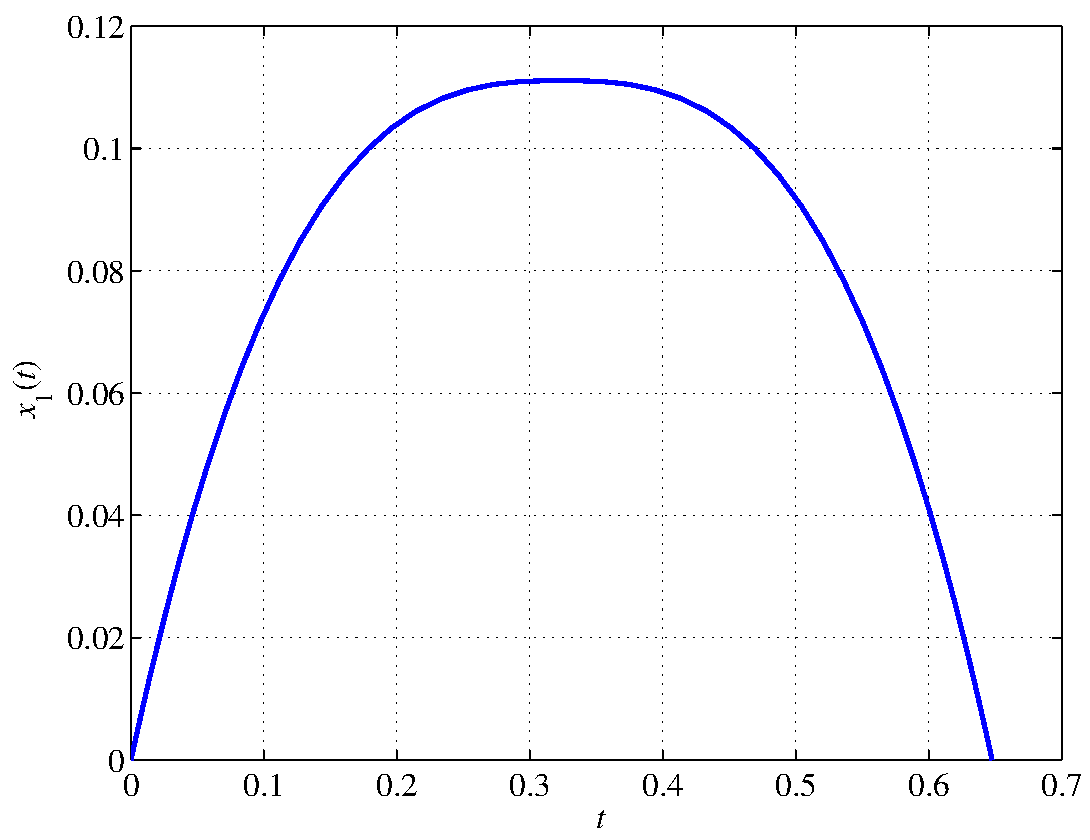
\includegraphics[height=3.5in]{x1vstBrysonDenham.pdf}
  \caption{$x_1(t)$ vs.~$t$ for Bryson-Denham problem.}
\end{figure}
\begin{figure}[H]
  \centering
  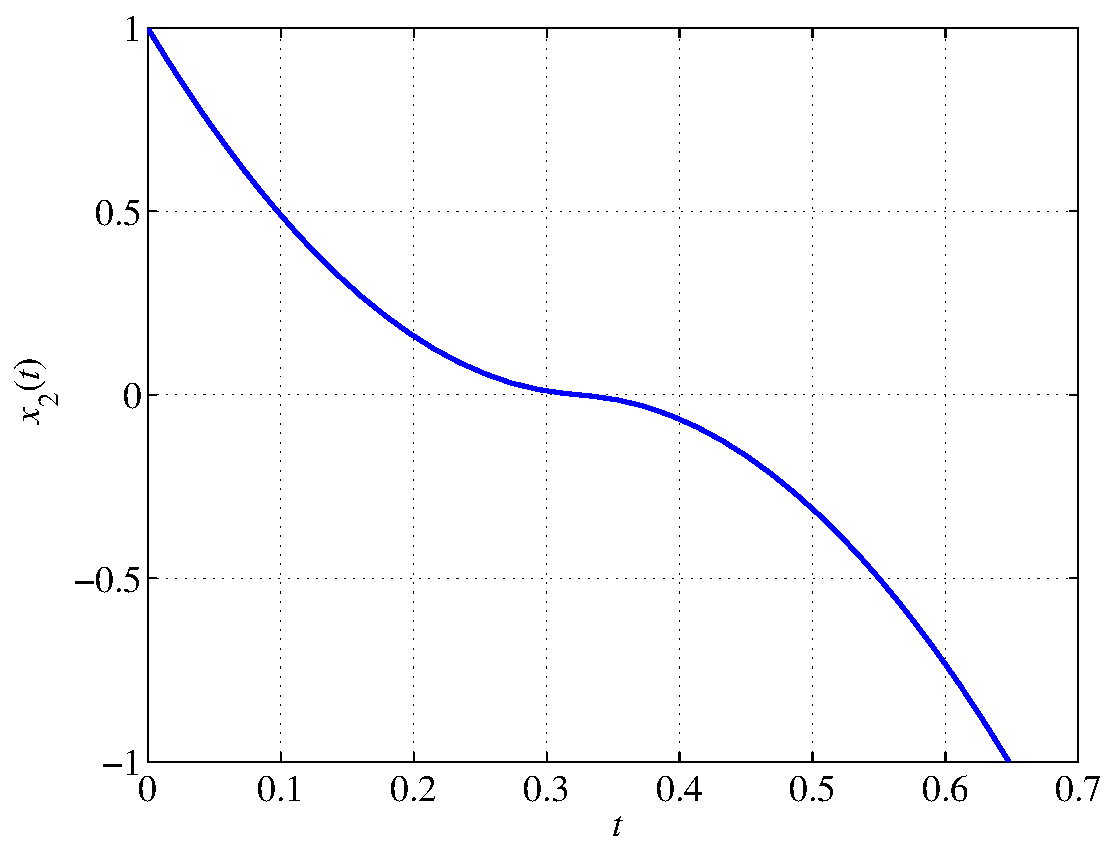
\includegraphics[height=3.5in]{x2vstBrysonDenham.pdf}
  \caption{$x_2(t)$ vs.~$t$ for Bryson-Denham problem.}
\end{figure}
\begin{figure}[H]
  \centering
  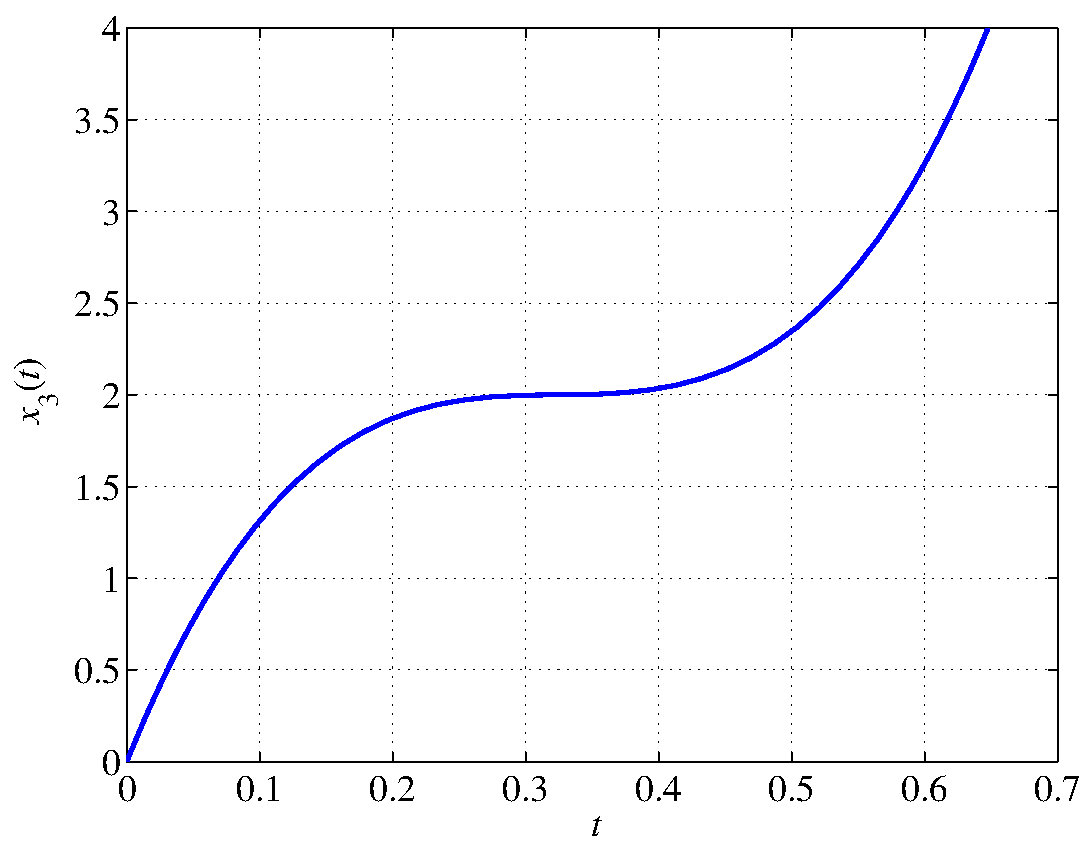
\includegraphics[height=3.5in]{x3vstBrysonDenham.pdf}
  \caption{$x_3(t)$ vs.~$t$ for Bryson-Denham problem.}
\end{figure}

\begin{figure}[H]
  \centering
  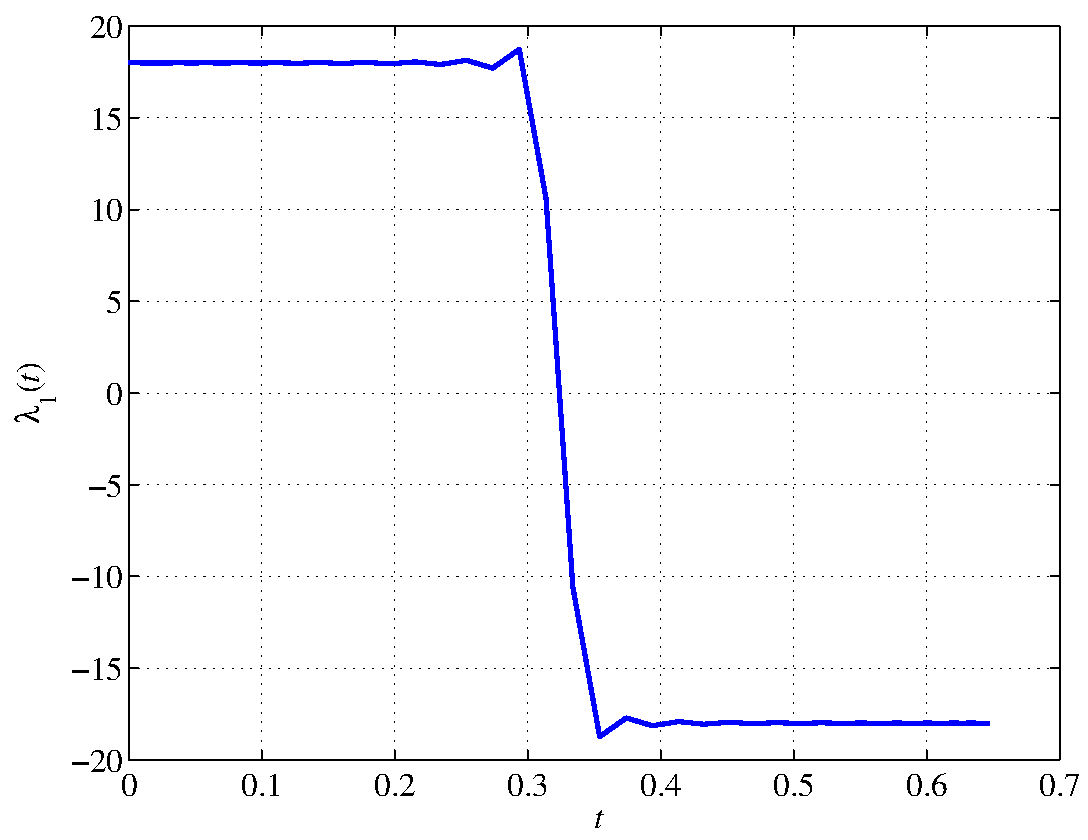
\includegraphics[height=3.5in]{lambda1vstBrysonDenham.pdf}
  \caption{$\lambda_1(t)$ vs.~$t$ for Bryson-Denham problem.}
\end{figure}
\begin{figure}[H]
  \centering
  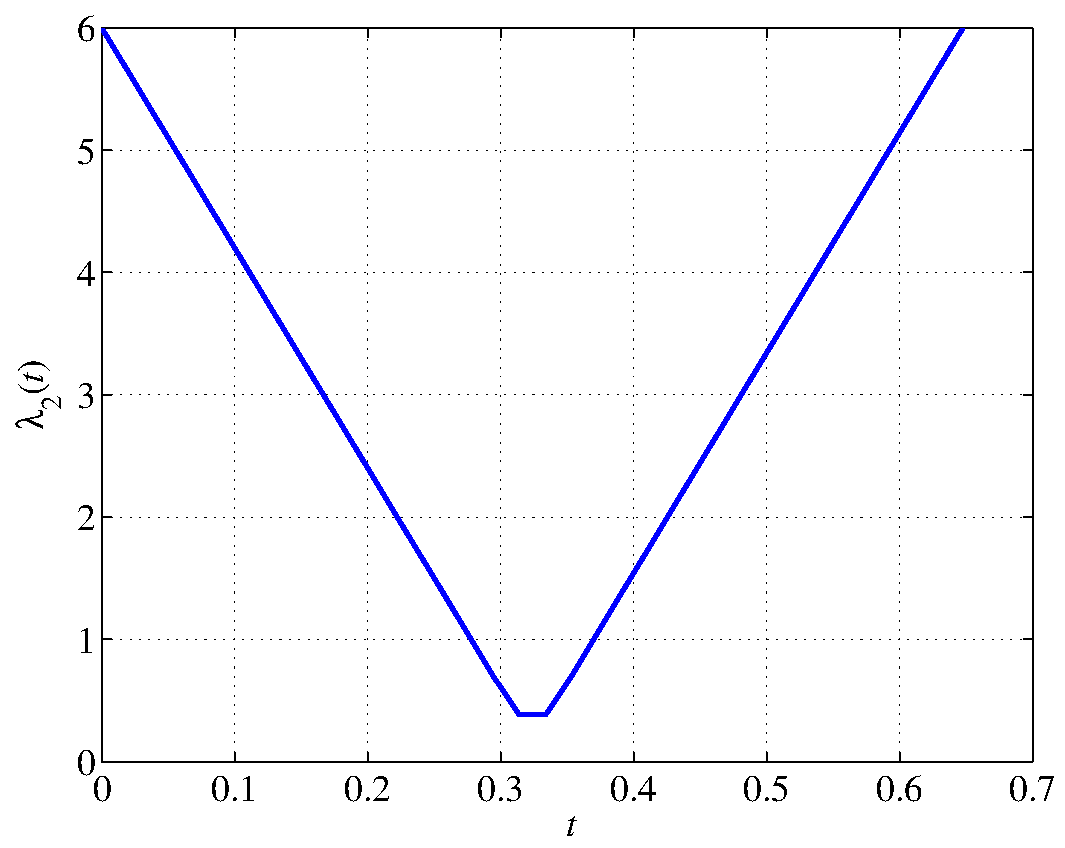
\includegraphics[height=3.5in]{lambda2vstBrysonDenham.pdf}
  \caption{$\lambda_2(t)$ vs.~$t$ for Bryson-Denham problem.}
\end{figure}
\begin{figure}[H]
  \centering
  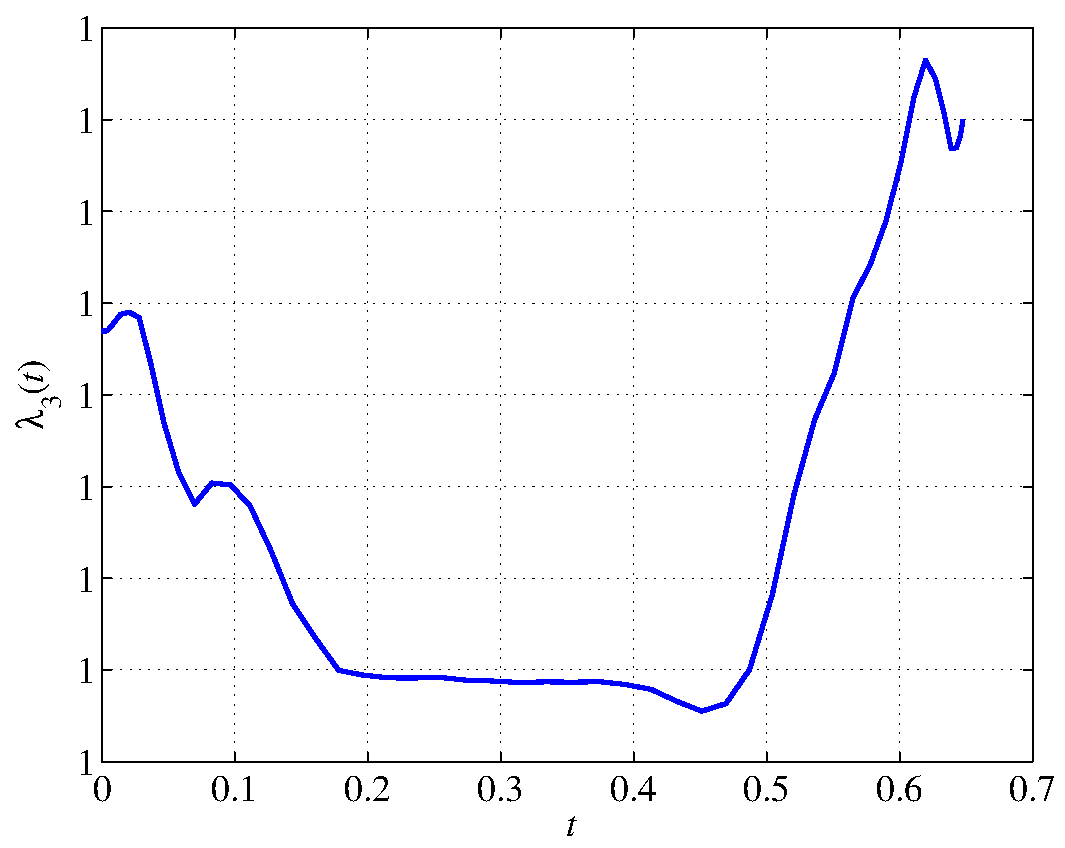
\includegraphics[height=3.5in]{lambda3vstBrysonDenham.pdf}
  \caption{$\lambda_3(t)$ vs.~$t$ for Bryson-Denham problem.}
\end{figure}
\begin{figure}[H]
  \centering
  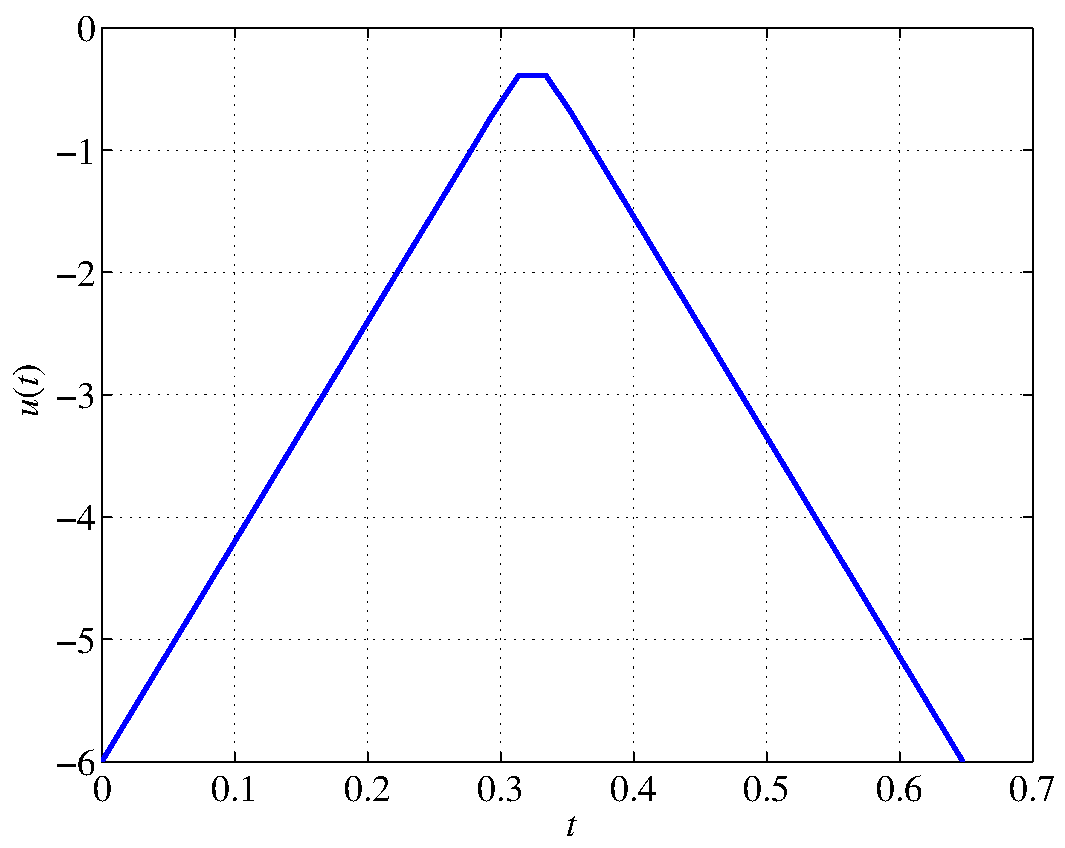
\includegraphics[height=3.5in]{uvstBrysonDenham.pdf}
  \caption{$u(t)$ vs.~$t$ for Bryson-Denham problem.}
\end{figure}

\section{Multiple-Stage Launch Vehicle Ascent Problem}

The problem considered in this section is the ascent of a
multiple-stage launch vehicle.  The objective is to maneuver the launch
vehicle from the ground to the target orbit while maximizing the remaining
fuel in the upper stage.   It is noted that this example is taken
verbatim from \citeasnoun{Benson1}.

\subsection{Vehicle Properties}

The launch vehicle considered in this example has two main stages
along with nine strap-on solid rocket boosters.  The flight of the
vehicle can be divided into {\em four} distinct phases.  The first
phase begins with the rocket at rest on the ground and at time $t_0$,
the main engine and six of the nine solid boosters ignite.  When the
boosters are depleted at time $t_1$, their remaining dry mass is
jettisoned. The final three boosters are then ignited, and along with the
main engine, represent the thrust for the second phase of flight.
These three remaining boosters are jettisoned when their fuel is
exhausted at time $t_2$, and the main engine alone creates the thrust
for the third phase.   The fourth phase begins when the main engine
fuel has been exhausted (MECO) and the dry mass associated with the
main engine is ejected at time $t_3$.   The thrust during phase four
is from a second stage, which burns until the target orbit has been
reached (SECO) at time $t_4$, thus completing the trajectory.  The
specific characteristics of these rocket motors can be seen in Table
\ref{table: launch vehicle properties}.  Note that the solid boosters
and main engine burn for their entire duration (meaning $t_1$, $t_2$,
and $t_3$ are fixed), while the second stage engine is shut off when
the target orbit is achieved ($t_4$ is free).

\begin{table}[htdp]
\centering
\caption{Mass and propulsion properties of the launch vehicle ascent
  problem. \label{table: launch vehicle properties}}
\begin{tabular}{|c|c|c|c|}
\hline
 & Solid Boosters & Stage 1 & Stage 2 \\
 \hline \hline
 Total Mass (kg) & 19290 & 104380 & 19300 \\
 \hline
 Propellant Mass (kg) & 17010 & 95550 & 16820 \\
 \hline
 Engine Thrust (N) & 628500 & 1083100 & 110094 \\
 \hline
 Isp (sec) & 284 & 301.7 & 462.4 \\
 \hline
 Number of Engines & 9 & 1 & 1 \\
 \hline
 Burn Time (sec) & 75.2 & 261 & 700 \\
 \hline
\end{tabular}
\end{table}

\subsection{Dynamic Model}

The equations of motion for a non-lifting point mass in flight over a
spherical rotating planet are expressed in Cartesian Earth centered inertial
(ECI) coordinates as
\begin{equation}\label{dyncs}
\begin{array}{rcl}
  \dot{\textbf{r}} &=& {\bf v} \vspace{3pt}\\
  \dot{\textbf{v}} &=& -\displaystyle\frac{\mu}{\|\textbf{r}\|^3}{\bf r} +
  \displaystyle\frac{T}{m}{\bf u} + \displaystyle\frac{{\bf D}}{m}  \vspace{3pt}\\
  \dot{m} & = & -\displaystyle\frac{T}{g_0I_{sp}}
\vspace{3pt}\\
\end{array}
\end{equation}
where ${\bf r}(t)=\left[\begin{array}{ccc} x(t) & y(t) & z(t)\end{array}\right]^T$
is the position, ${\bf v} = \left[\begin{array}{ccc} v_x(t) & v_y(t) & v_z(t)\end{array}\right]^T$
is the Cartesian ECI velocity, $\mu$ is the gravitational parameter, $T$ is
the vacuum thrust, $m$ is the mass, $g_0$ is the acceleration due to gravity at sea level,
$I_{sp}$ is the specific impulse of the engine,
${\bf u} = \left[\begin{array}{ccc} u_x & u_y & u_z \end{array}\right]^T$ is the thrust
direction, and ${\bf D}=\left[\begin{array}{ccc} D_x & D_y & D_z \end{array}\right]^T$
is the drag force.  The drag force is defined as
\begin{equation}
  {\bf D} = -\frac{1}{2}C_D A_{ref}\rho \|{\bf v}_{rel}\|{\bf v}_{rel}
\end{equation}
where $C_D$ is the drag coefficient, $A_{ref}$ is the reference area, $\rho$
is the atmospheric density, and ${\bf v}_{rel}$ is the Earth relative
velocity, where ${\bf v}_{rel}$ is given as
\begin{equation}
{\bf v}_{rel} = {\bf v}-\boldsymbol{\omega} \times {\bf r}
\end{equation}
where $\boldsymbol\omega$ is the angular velocity of the Earth relative to
inertial space.  The atmospheric density is modeled as the exponential
function
\begin{equation}
\rho = \rho_0\mbox{exp}[-h/h_0]
\end{equation}
where $\rho_0$ is the atmospheric density at sea level, $h=\|\bfr\|-R_e$ is
the altitude, $R_e$ is the equatorial radius of the Earth, and $h_0$ is the
density scale height.  The numerical values for these constants can be found
in Table \ref{dynamics properties}.

%This dynamic model has many simplifying assumptions.  First, the thrust from
%each engine is assumed to be the vacuum thrust.  This results in a constant
%thrust magnitude that does not depend on atmospheric pressure.  Second, the
%reference area and coefficient of drag are constant for the entire trajectory,
%with no dependence on Mach number or angle of attack.  Third, the drag is
%assumed to always oppose the relative velocity.  There is no component of
%lift, and the drag has no dependence on vehicle orientation.  Lastly, the
%Earth is modeled as a perfect sphere.   These assumptions allow the dynamic
%equations to be the same for each phase of the trajectory, where only the
%thruster characteristics change between phases.

\begin{table}[htdp]
\caption{Constants used in the launch vehicle example.}
\begin{center}
\begin{tabular}{|c|c|}
\hline
Constant & Value \\
\hline \hline
Payload Mass (kg) & 4164 \\
\hline
$A_{ref}$ (m${}^2$) & $4\pi$ \\
\hline
$C_d$ & 0.5 \\
\hline
$\rho_0$ (kg/m${}^3$)& 1.225 \\
\hline
$h_0$ (km) & 7.2\\
\hline
$t_1$ (s) & 75.2 \\
\hline
 $t_2$ (s) & 150.4 \\
\hline
 $t_3$ (s) & 261 \\
\hline
 $R_e$ (km) & 6378.14 \\
\hline
 $V_E$ (km/s) & 7.905\\
\hline
\end{tabular}
\end{center}
\label{dynamics properties}
\end{table}

\subsection{Constraints}
The launch vehicle starts on the ground at rest (relative to the Earth) at time $t_0$, so that the ECI initial conditions are
\begin{equation}\label{ICs}
\begin{array}{rcl}
{\bf r}(t_0) &=& {\bf r}_0 = \left[ \begin{array}{ccc} 5605.2 & 0 & 3043.4 \end{array} \right] ^T\quad \mbox{km} \vspace{3pt}\\
{\bf v}(t_0) &=& {\bf v}_0 = \left[ \begin{array}{ccc} 0 & 0.4076 & 0 \end{array} \right]^T \quad \mbox{km/s} \vspace{3pt}\\
m(t_0) &=& m_0 = 301454 \quad \mbox{kg}
\end{array}
\end{equation}
which corresponds to the Cape Canaveral launch site.  The terminal constraints
define the target geosynchronous transfer orbit (GTO), which is defined in
orbital elements as
\begin{equation}\label{FCs}
\begin{array}{rcl}
 a_f &=   &  24361.14 \; \mbox{km}, \\
 e_f &=   &  0.7308, \\
 i_f &=   &  28.5\deg,\\
 \Omega_f &= & 269.8\deg, \\
 \omega_f &= & 130.5\deg
\end{array}
\end{equation}
The orbital elements, $a,e,i,\Omega$, and $\omega$ represent the semi-major
axis, eccentricity, inclination, right ascension of the ascending node
(RAAN), and argument of perigee, respectively.  Note that the true anomaly,
$\nu$, is left undefined since the exact location within the orbit is not
constrained.  These orbital elements can be transformed into ECI coordinates
via the transformation, $T_{o2c}$, where $T_{o2c}$ is given in \cite{Bate1}.

In addition to the boundary constraints, there exists both a state path
constraint and a control path constraint in this problem.  A state path
constraint is imposed to keep the vehicle's altitude above the surface of the
Earth, so that
\begin{equation}\label{xpath}
|{\bf r}|\geq R_r
\end{equation}
where $R_e$ is the radius of the Earth, as seen in Table \ref{dynamics
  properties}.  Next, a path constraint is imposed on the control to guarantee
that the control vector is unit length, so that
\begin{equation}\label{upath}
|{\bf u}| = 1
\end{equation}

Lastly, each of the four phases in this trajectory is linked to the adjoining phases by a set of linkage conditions.  These constraints force the position and velocity to be continuous and also account for the mass ejections, as
\begin{equation}
\begin{array}{rcl}
{\bf r}^{(p)}(t_f)-{\bf r}^{(p+1)}(t_0) &=& {\bf 0}, \\
{\bf v}^{(p)}(t_f)-{\bf v}^{(p+1)}(t_0) &=& {\bf 0}, \qquad (p=1,\ldots,3)\\
m^{(p)}(t_f)-m_{dry}^{(p)}-m^{(p+1)}(t_0) &=& 0 \\
\end{array}
\end{equation}
where the superscript $(p)$ represents the phase number.

The optimal control problem is then to find the control, ${\bf u}$,
that minimizes the cost function
\begin{equation}
  J=-m^{(4)}(t_f)
\end{equation}
subject to the conditions of Eqs.~(\ref{dyncs}), (\ref{ICs}), (\ref{FCs}),
(\ref{xpath}), and (\ref{upath}).

The MATLAB code that solves the multiple-stage launch vehicle ascent
problem using \gpops is shown below.  In particular, this
problem requires the specification of a function that computes the
cost functional, the differential-algebraic equations (which, it is
noted, include both the differential equations {\em and} the path
constraints), and the event constraints in each phase of the problem
along with the phase-connect (\ie linkage) constraints.  The problem
was posed in SI units and the built-in autoscaling procedure was
used.
\footnotesize
\begin{shadedframe}
\verbatiminput{../examples/launch/launchMain.m}
\verbatiminput{../examples/launch/launchCost.m}
\verbatiminput{../examples/launch/launchDae.m}
\verbatiminput{../examples/launch/launchEvent.m}
\verbatiminput{../examples/launch/launchrv2oe.m}
\verbatiminput{../examples/launch/launchoe2rv.m}
\end{shadedframe}
\normalsize
The output of the above code from \gpops is summarized in the following three
plots that contain the altitude, speed, and controls.
\begin{figure}[H]
  \centering
  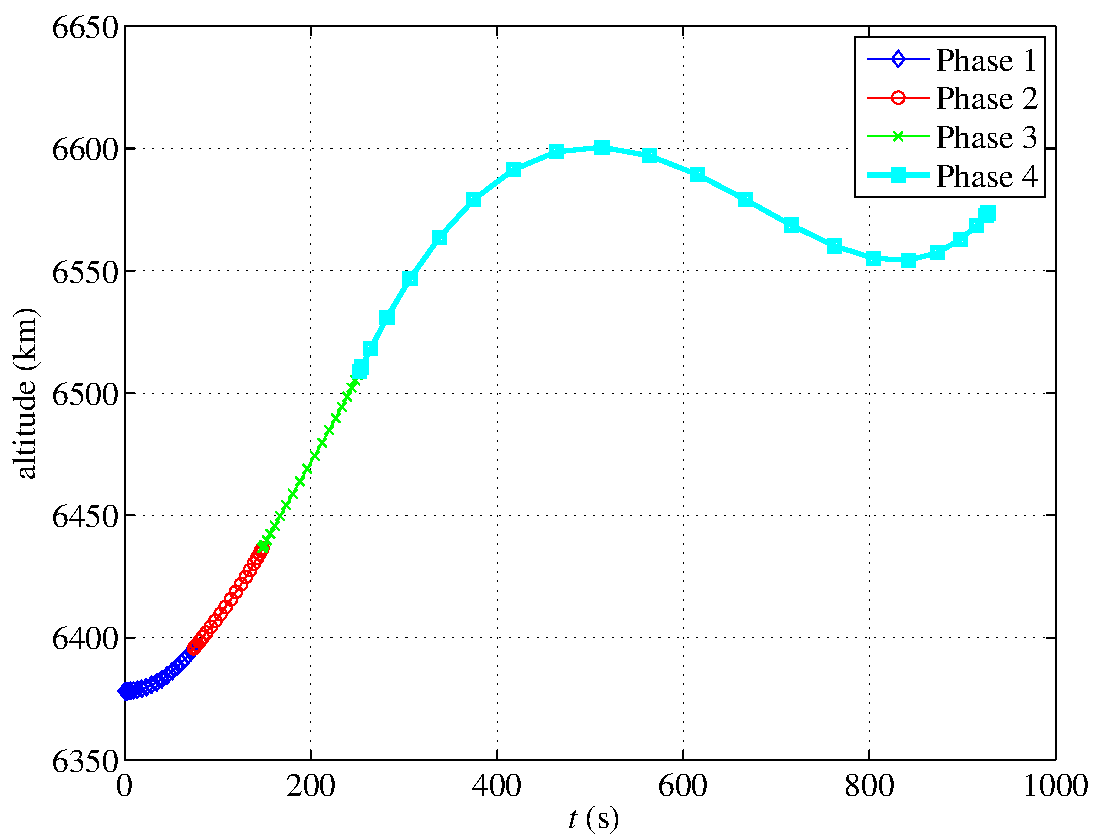
\includegraphics[height=3.5in]{altitudevstLaunch.pdf}
  \caption{Altitude vs.~time for the launch vehicle ascent problem.}
\end{figure}
\begin{figure}[H]
  \centering
  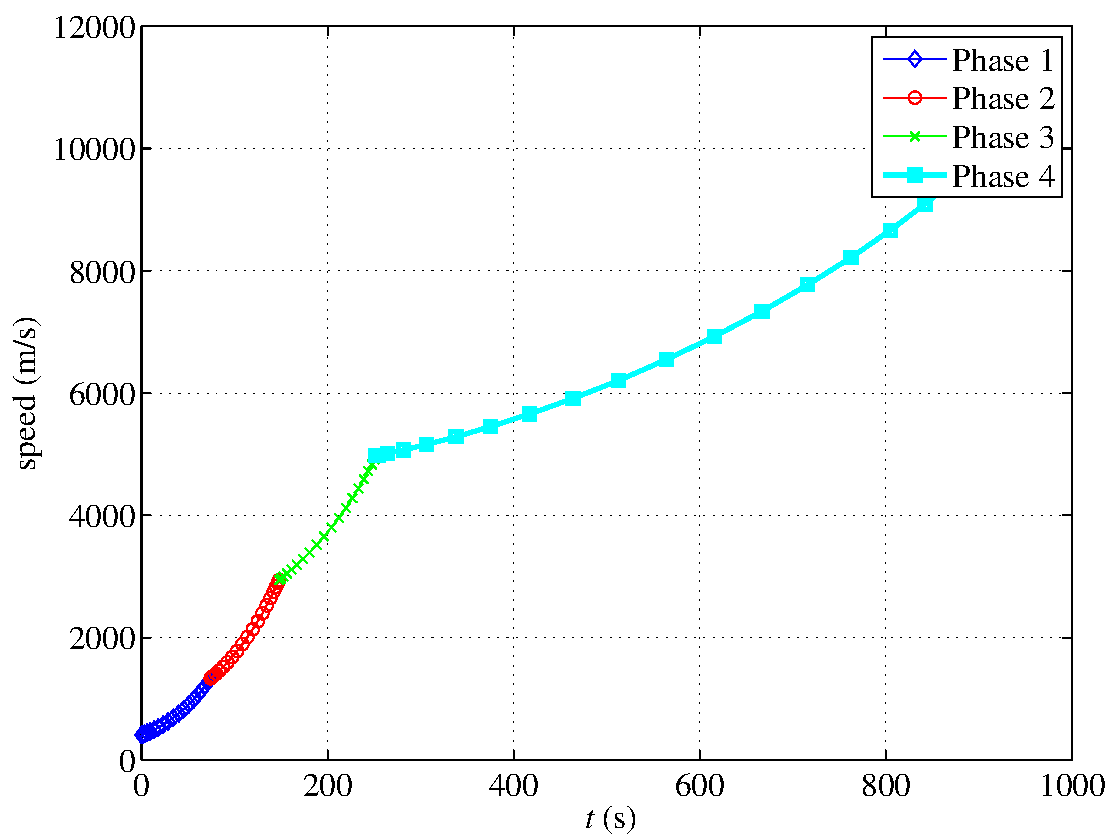
\includegraphics[height=3.5in]{speedvstLaunch.pdf}
  \caption{Inertial speed vs.~time for the launch vehicle ascent problem.}
\end{figure}
\begin{figure}[H]
  \centering
  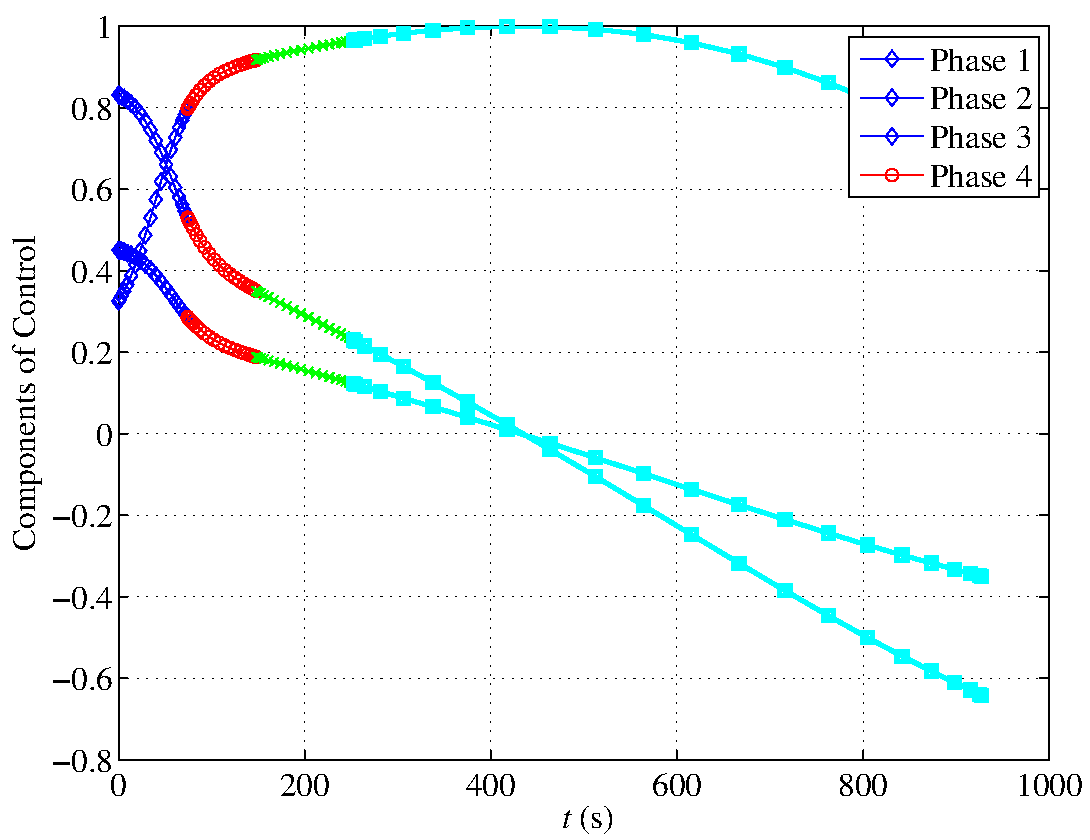
\includegraphics[height=3.5in]{uvstLaunch.pdf}
  \caption{Controls vs.~time for the launch vehicle ascent problem.}
\end{figure}

\section{Minimum Time-to-Climb of a Supersonic Aircraft}

The problem considered in this section is the classical minimum
time-to-climb of a supersonic aircraft.  The objective is to determine
the minimum-time trajectory and control from take-off to a specified
altitude and speed.  This problem was originally stated in the open
literature in the work of \citeasnoun{Bryson1}, but the model used in
this study was taken from \citeasnoun{Betts1} with the exception that
a linear extrapolation of the thrust data as found in
\citeasnoun{Betts1} was performed in order to fill in the ``missing''
data points.

The minimum time-to-climb problem for a supersonic aircraft is posed
as follows.  Minimize the cost functional
\begin{equation}
  J = t_f
\end{equation}
subject to the dynamic constraints
\begin{eqnarray}
  \dot{E} & = & \frac{v(T-D)}{mg} \\
  \dot{h} & = & v\sin\gamma \\
  \dot{\gamma} & = & \frac{g}{v}\left[n-\cos\gamma\right] \\
\end{eqnarray}
and the boundary conditions
\begin{eqnarray}
  h(0) & = & 0 \textrm{ ft} \\
  v(0) & = & 129.3144 \textrm{ m/s} \\
  \gamma(0) & = & 0 \textrm{ rad} \\
  h(t_f) & = & 19995 \textrm{ m} \\
  v(t_f) & = & 295.09 \textrm{ ft/s} \\
  \gamma(t_f) & = & 0 \textrm{ rad}
\end{eqnarray}
where $E$ is the the energy altitude, $h$ is the altitude, $\gamma$ is the
flight path angle, $m$ is the vehicle mass, $n$ is the load factor,
$T$ is the magnitude of the thrust force, and $D$ is the magnitude
of the drag force.

The MATLAB code that solves the minimum time-to-climb of a supersonic
aircraft is shown below.
\footnotesize
\begin{shadedframe}
\verbatiminput{../examples/minimumClimb/minimumClimbMain.m}
\verbatiminput{../examples/minimumClimb/minimumClimbCost.m}
\verbatiminput{../examples/minimumClimb/minimumClimbDae.m}
\verbatiminput{../examples/minimumClimb/minimumClimbDae.m}
\end{shadedframe}
\normalsize
The output of the above code from \gpops is summarized in the
following three plots that contain the altitude, speed, flight path
angle, and angle of attack:
\begin{figure}[H]
  \centering
  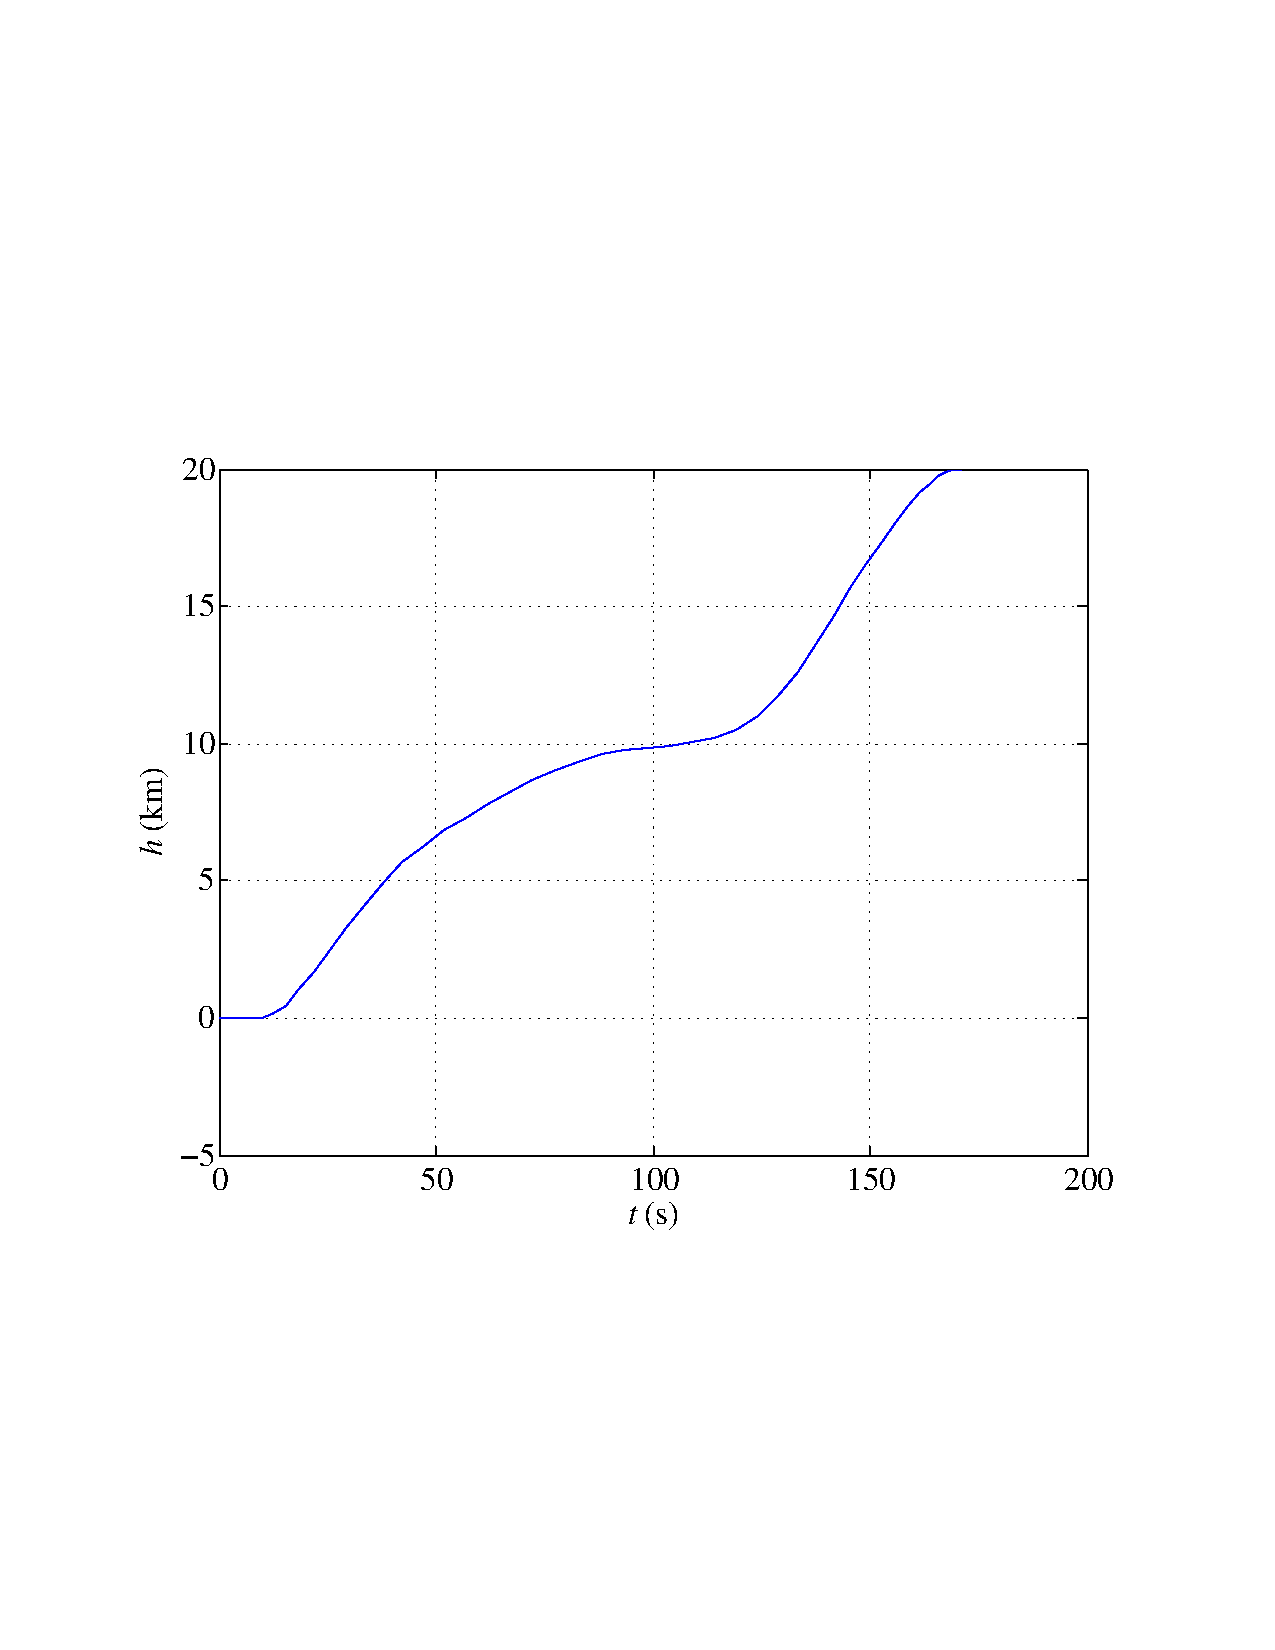
\includegraphics[height=3.5in]{hvstMinClimb.pdf}
  \caption{Altitude vs.~Time for supersonic aircraft minimum time-to-climb.}
\end{figure}
\begin{figure}[H]
  \centering
  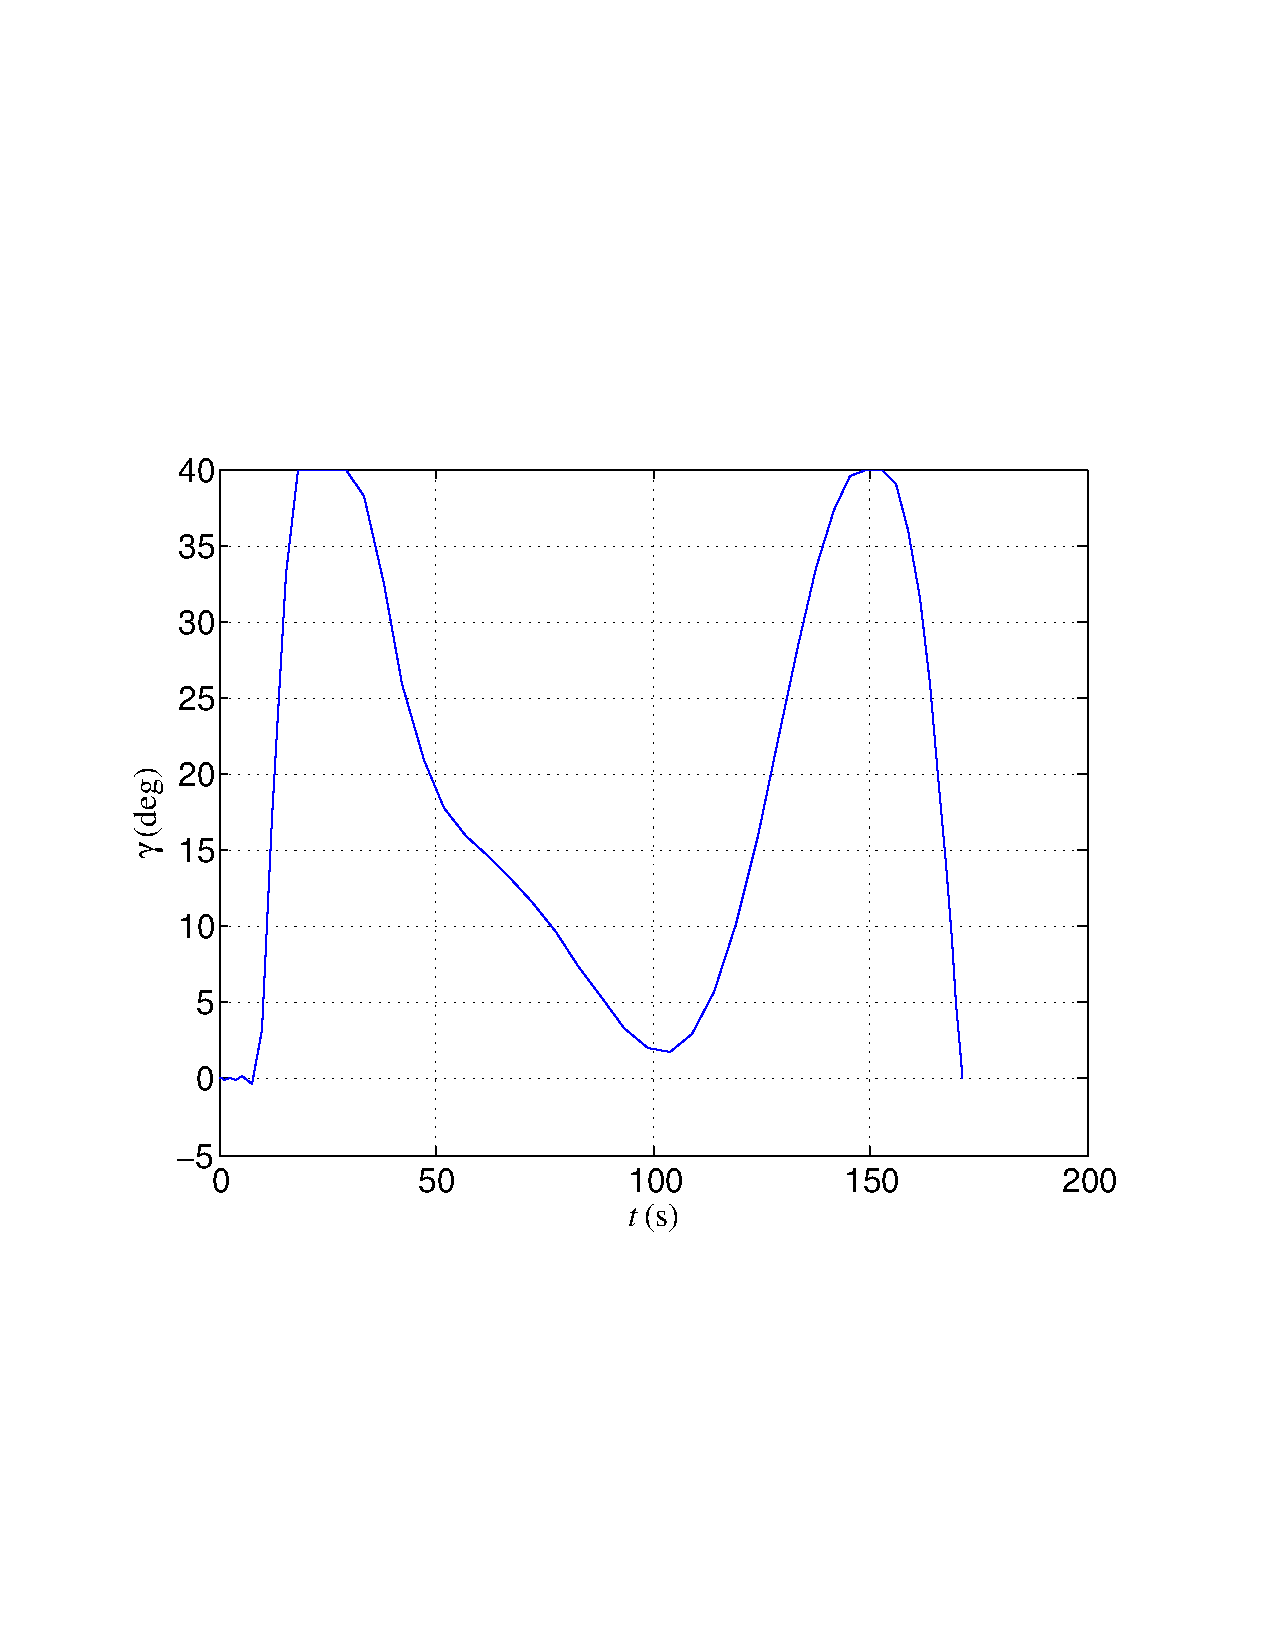
\includegraphics[height=3.5in]{fpavstMinClimb.pdf}
  \caption{Flight path angle vs.~Time for supersonic aircraft minimum time-to-climb.}
\end{figure}
\begin{figure}[H]
  \centering
  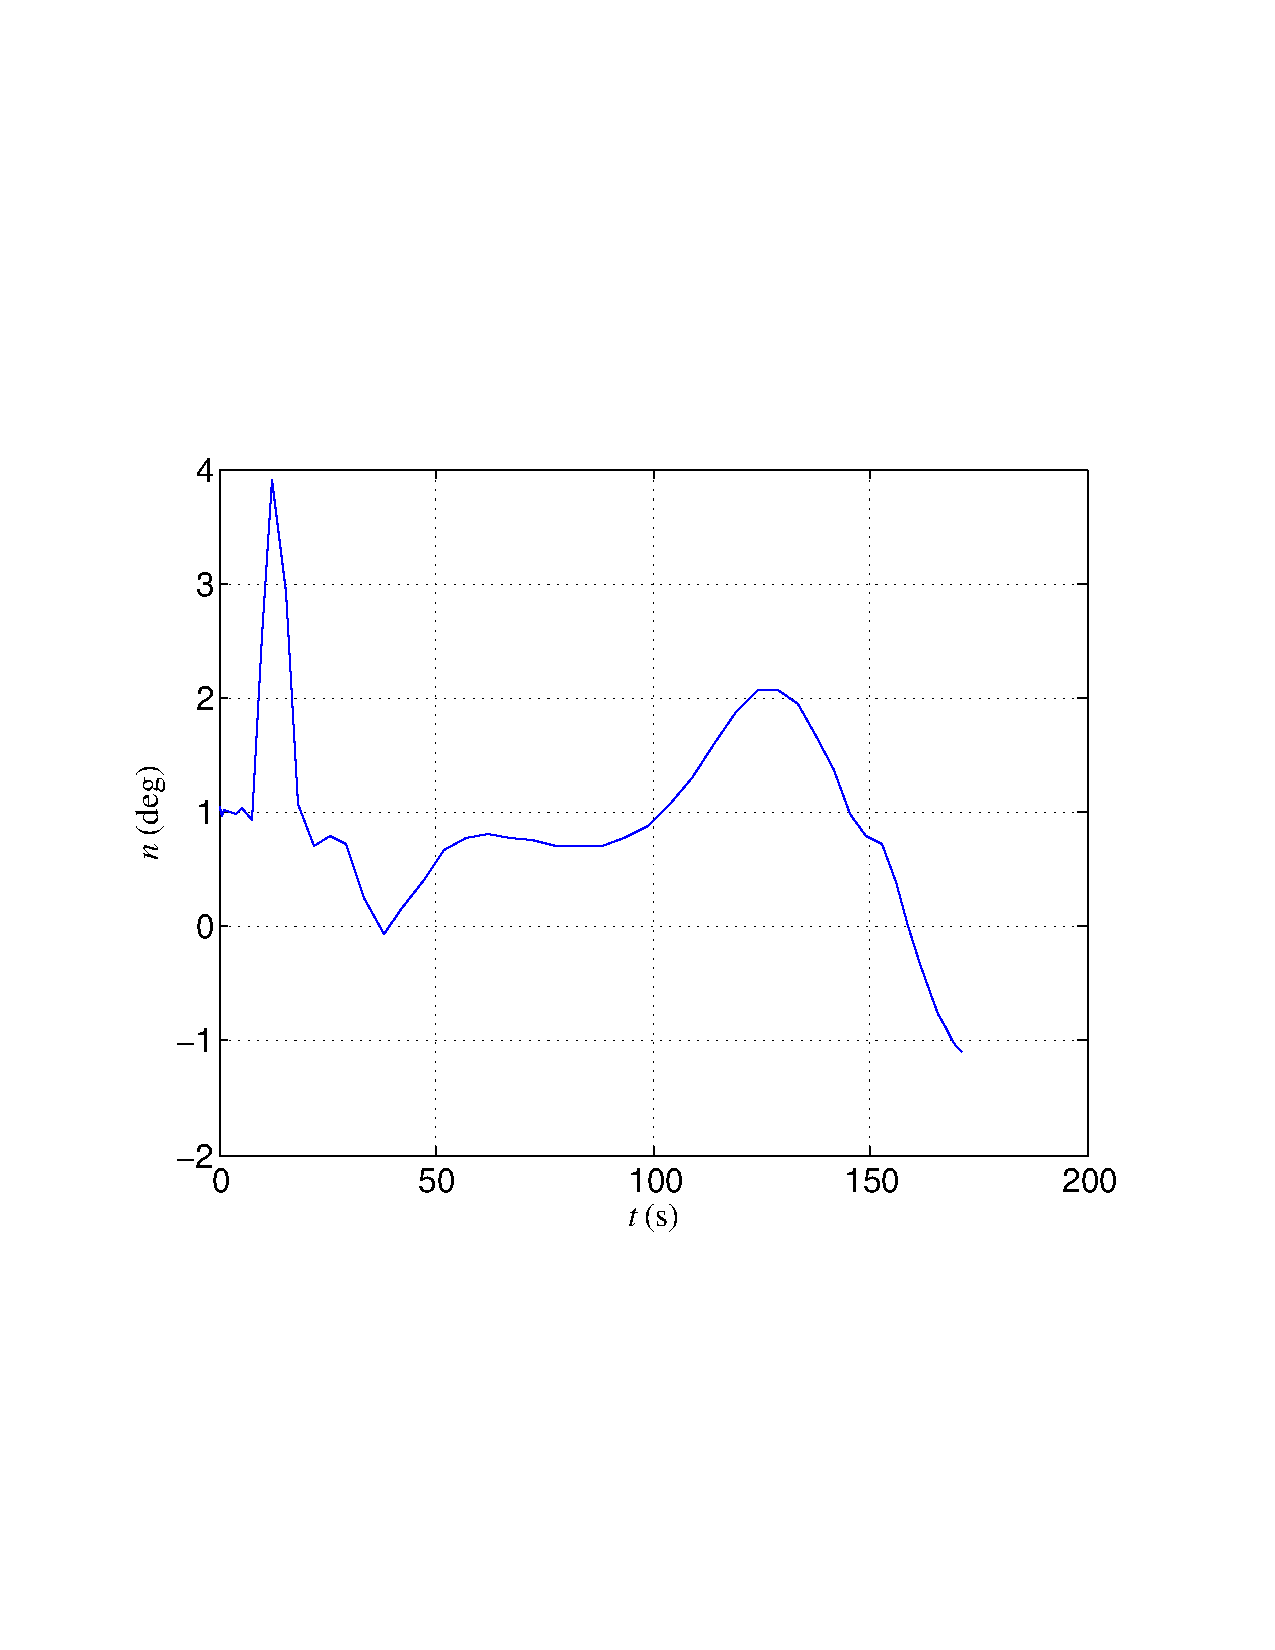
\includegraphics[height=3.5in]{nvstMinClimb.pdf}
  \caption{Angle of attack vs.~Time for supersonic aircraft minimum time-to-climb.}
\end{figure}

\section{Some Concluding Remarks}

While \gpops has been designed to take some of the cumbersomeness out of
solving an optimal control problem numerically, the user must still be wary of
several aspects of computational optimal control that will make it easier to
use \gpops.  First, as noted earlier, it is {\em highly} recommended that
the user scale the problem manually because the automatic scaling procedure is
by no means foolproof.  Second, the choice of variables to solve an optimal
control problem can make all the difference in the world as to how quickly and
reliably a solution is obtained.  For example, atmospheric flight problems
with large lift maneuvers tend to be easier to solve if spherical coordinates
(where position is parameterized using radius, longitude, and latitude, while
velocity is parameterized using speed, flight path angle, and heading angle)
are used as compared to Cartesian coordinates whereas launch vehicle ascent
problems (which have no lift) tend to be better parameterized using Cartesian
coordinates.  Finally, even if the optimizer returns the result that the
optimality conditions have been satisfied, it is extremely important to
analyze the solution to make sure that (1) the solution is the one
corresponding to the problem that the user wants to solve and (2) if the
solution makes sense.  In short, a great deal of time in solving optimal
control problems is spent in formulation and analysis.

\begin{thebibliography}{}

  \harvarditem{Bate, et~al.}{2001}{Bate1} Bate, R.~R., Mueller, D.~D., and
  White, J.~E., {\em Fundamentals of Astrodynamics}, Dover Publications, New
  York, 1971.

  \harvarditem{Benson}{2004}{Benson1} Benson, D.~A., {\em A Gauss
    Pseudospectral Transcription for Optimal Control}, Ph.D.~Dissertation,
  Department of Aeronautics and Astronautics, MIT, November 2004.

  \harvarditem{Benson, et~al.}{2006}{Benson2} Benson, D.~A., Huntington,
  G.~T., Thorvaldsen, T.~P., and Rao, A.~V., ``Direct Trajectory
  Optimization and Costate Estimation via an Orthogonal Collocation
  Method,'', {\em Journal of Guidance, Control, and Dynamics},
  Vol.~29, No.~6, November-December, 2006, pp.~1435--1440.

  \harvarditem{Betts}{2001}{Betts1} Betts, J.~T., {\em Practical Methods for
    Optimal Control Using Nonlinear Programming}, SIAM Press, Philadelphia,
  2001.

  \harvarditem{Bryson, et~al.}{1963}{Bryson2} Bryson, A.~E., Denham, W.~F.,
  and Dreyfus, S.~E., ``Optimal Programming Problems with Inequality Constraints.
  I: Necessary Conditions for Extremal Solutions'', {\em AIAA Journal}, Vol.~1, No.~11,
  November 1963, pp.~2544-2550.

  \harvarditem{Bryson, et~al.}{1969}{Bryson1} Bryson, A.~E., Desai,
  M.~N., and Hoffman, W.~C., ``Energy-State Approximation in
  Performance Optimization of Supersonic Aircraft,'' {\em Journal of
    Aircraft}, Vol.~6, No.~6, 1969, pp.~481--488.

  \harvarditem{Davis}{1975}{Davis1} Davis, P.,  {\em Interpolation and
    Approximation}, Dover Publications, 1975.

  \harvarditem{Elnagar, et~al.}{1995}{Elnagar1} Elnagar, G., Kazemi, M., Razzaghi,
  M., ``The Pseudospectral Legendre Method for Discretizing Optimal Control
  Problems," {\em IEEE Transactions on Automatic Control} Vol.~40, No.~10,
  October 1995.

  \harvarditem{Elnagar and Kazemi}{1998}{Elnagar2} Elnagar, G.~ and Kazemi, M.,
  ``Pseudospectral Chebyshev Optimal Control of Constrained Nonlinear
  Dynamical Systems," {\em Computational Optimization and Applications},
  Vol.~11, 1998, pp.~195-217.

  \harvarditem{Gill, et.~al.}{2007}{Gill1} Gill, P.~E., Murray, W.,
  and Saunders, M.~A., ``User's Guide for SNOPT Version 7:  Software
  for Large-Scale Nonlinear Programming,'' Report, University of
  California, San Diego, 24 April 2007.

  \harvarditem{Huntington, et~al.}{2005a}{Huntington1} Huntington, G.~T.~and Rao,
  A.~V., ``Optimal Spacecraft Formation Configuration Using a Gauss
  Pseudospectral Method,'' {\em Proceedings of the 2005 AAS/AISS
  Spaceflight Mechanics Meeting}, AAS Paper 05-103, Copper Mountain,
  Colorado, January 23--27, 2005.

  \harvarditem{Huntington, et~al.}{2005b}{Huntington2} Huntington, G.~T., Benson,
  D.~A., and Rao, A.~V., ``Post-Optimality Evaluation and Analysis of a
  Formation Flying Problem via a Gauss Pseudospectral Method,'' {\em
  Proceedings of the 2005 AAS/AIAA Astrodynamics Specialist
  Conference}, AAS Paper 05-339, Lake Tahoe, California, August 7--11,
  2005.

  \harvarditem{Huntington, et~al.}{2005c}{Huntington3} Huntington, G.~T.~and Rao, A.~V.,
  ``Optimal Reconfiguration of a Spacecraft Formation via a Gauss
  Pseudospectral Method,'' {\em Proceedings of the 2005 AAS/AIAA
  Astrodynamics Specialist Conference}, AAS Paper 05-338, Lake Tahoe,
  California, August 7--11, 2005.

  \harvarditem{Huntington}{2007}{Huntington6} Huntington, G.~T., {\em
    Advancement and Analysis of a Gauss Pseudospectral Transcription
    for Optimal Control}, Ph.D.~Dissertation, Department of
  Aeronautics and Astronautics, MIT, May 2007.

  \harvarditem{Huntington and Rao}{2007a}{Huntington4} Huntington, G.~T.~and Rao,
  A.~V., ``Design of Optimal Tetrahedral Spacecraft Formations,'' {\em The
    Journal of the Astronautical Sciences}, to appear in 2007.

  \harvarditem{Huntington, et.~al.}{2007b}{Huntington5} Huntington, G.~T.,
  Benson, D.~A., How, J.~P., Kanizay, N., Darby, C.~L., and Rao,
  A.~V., ``Computation of Boundary Controls Using a Gauss Pseudospectral
  Method,'' {\em 2007 Astrodynamics Specialist Conference}, Mackinac Island,
  Michigan, AAS Paper 07-381, August 21--24, 2007.

  %\harvarditem{Huntington, et~al.}{2007c}{Huntington7} Huntington, G.~T.,
  %Benson, D.~A., and Rao, A.~V., ``A Comparison of Accuracy and
  %Computational Efficiency of Three Pseudospectral Methods,''
  %{\em 2007 Guidance, Navigation, and Control Conference}, Hilton
  %Head, South Carolina,  AIAA Paper 2007-6405, August 21--24, 2007.

  \harvarditem{Kirk}{1970}{Kirk1} Kirk, D.~E., {\em Optimal Control Theory},
  Dover Publications, 1970.

  \harvarditem{Martins, et~al.}{2003}{Martins1} Martins, J.~R.~R.,
  Sturdza, P., and Alonso, J.~J., ``The Complex-Step Derivative
  Approximation,'' {\em ACM Transactions on Mathematical Software},
  Vol.~29, No.~3, 2003, pp.~245--262.

  \harvarditem{Pontryagin, et~al.}{1962}{Pontryagin1} Pontryagin, L.S., Boltyanskii,
  V., Gamkrelidze, R., Mischenko, E., {\em The Mathematical Theory of
    Optimal Processes}, New York: Interscience, 1962.

  \harvarditem{Rao}{2000}{Rao1} Rao, A.~V.~and Mease, K.~D., ``Eigenvector
  Approximate Dichotomic Basis Method for Solving Hyper-Sensitive Optimal
  Control Problems,'' {\em Optimal Control Applications and Methods},
    Vol.~21, No.~1, 2000, pp.~1--19.

\end{thebibliography}

\end{document}
